\chapter{تحليل المتطلبات}

\begin{chaptersummary}
نبين في هذا الفصل مخططات حالات الاستخدام والسرد النصي لها إضافة إلى تبيين مخططات تسلسل النظام لها
\end{chaptersummary}

\section{مخططات حالات الاستخدام \en{Use Case Diagrams}}

\subsection{حالات الاستخدام المستخدمين غير المسجلين}

\begin{figure}[H]
  \centering
  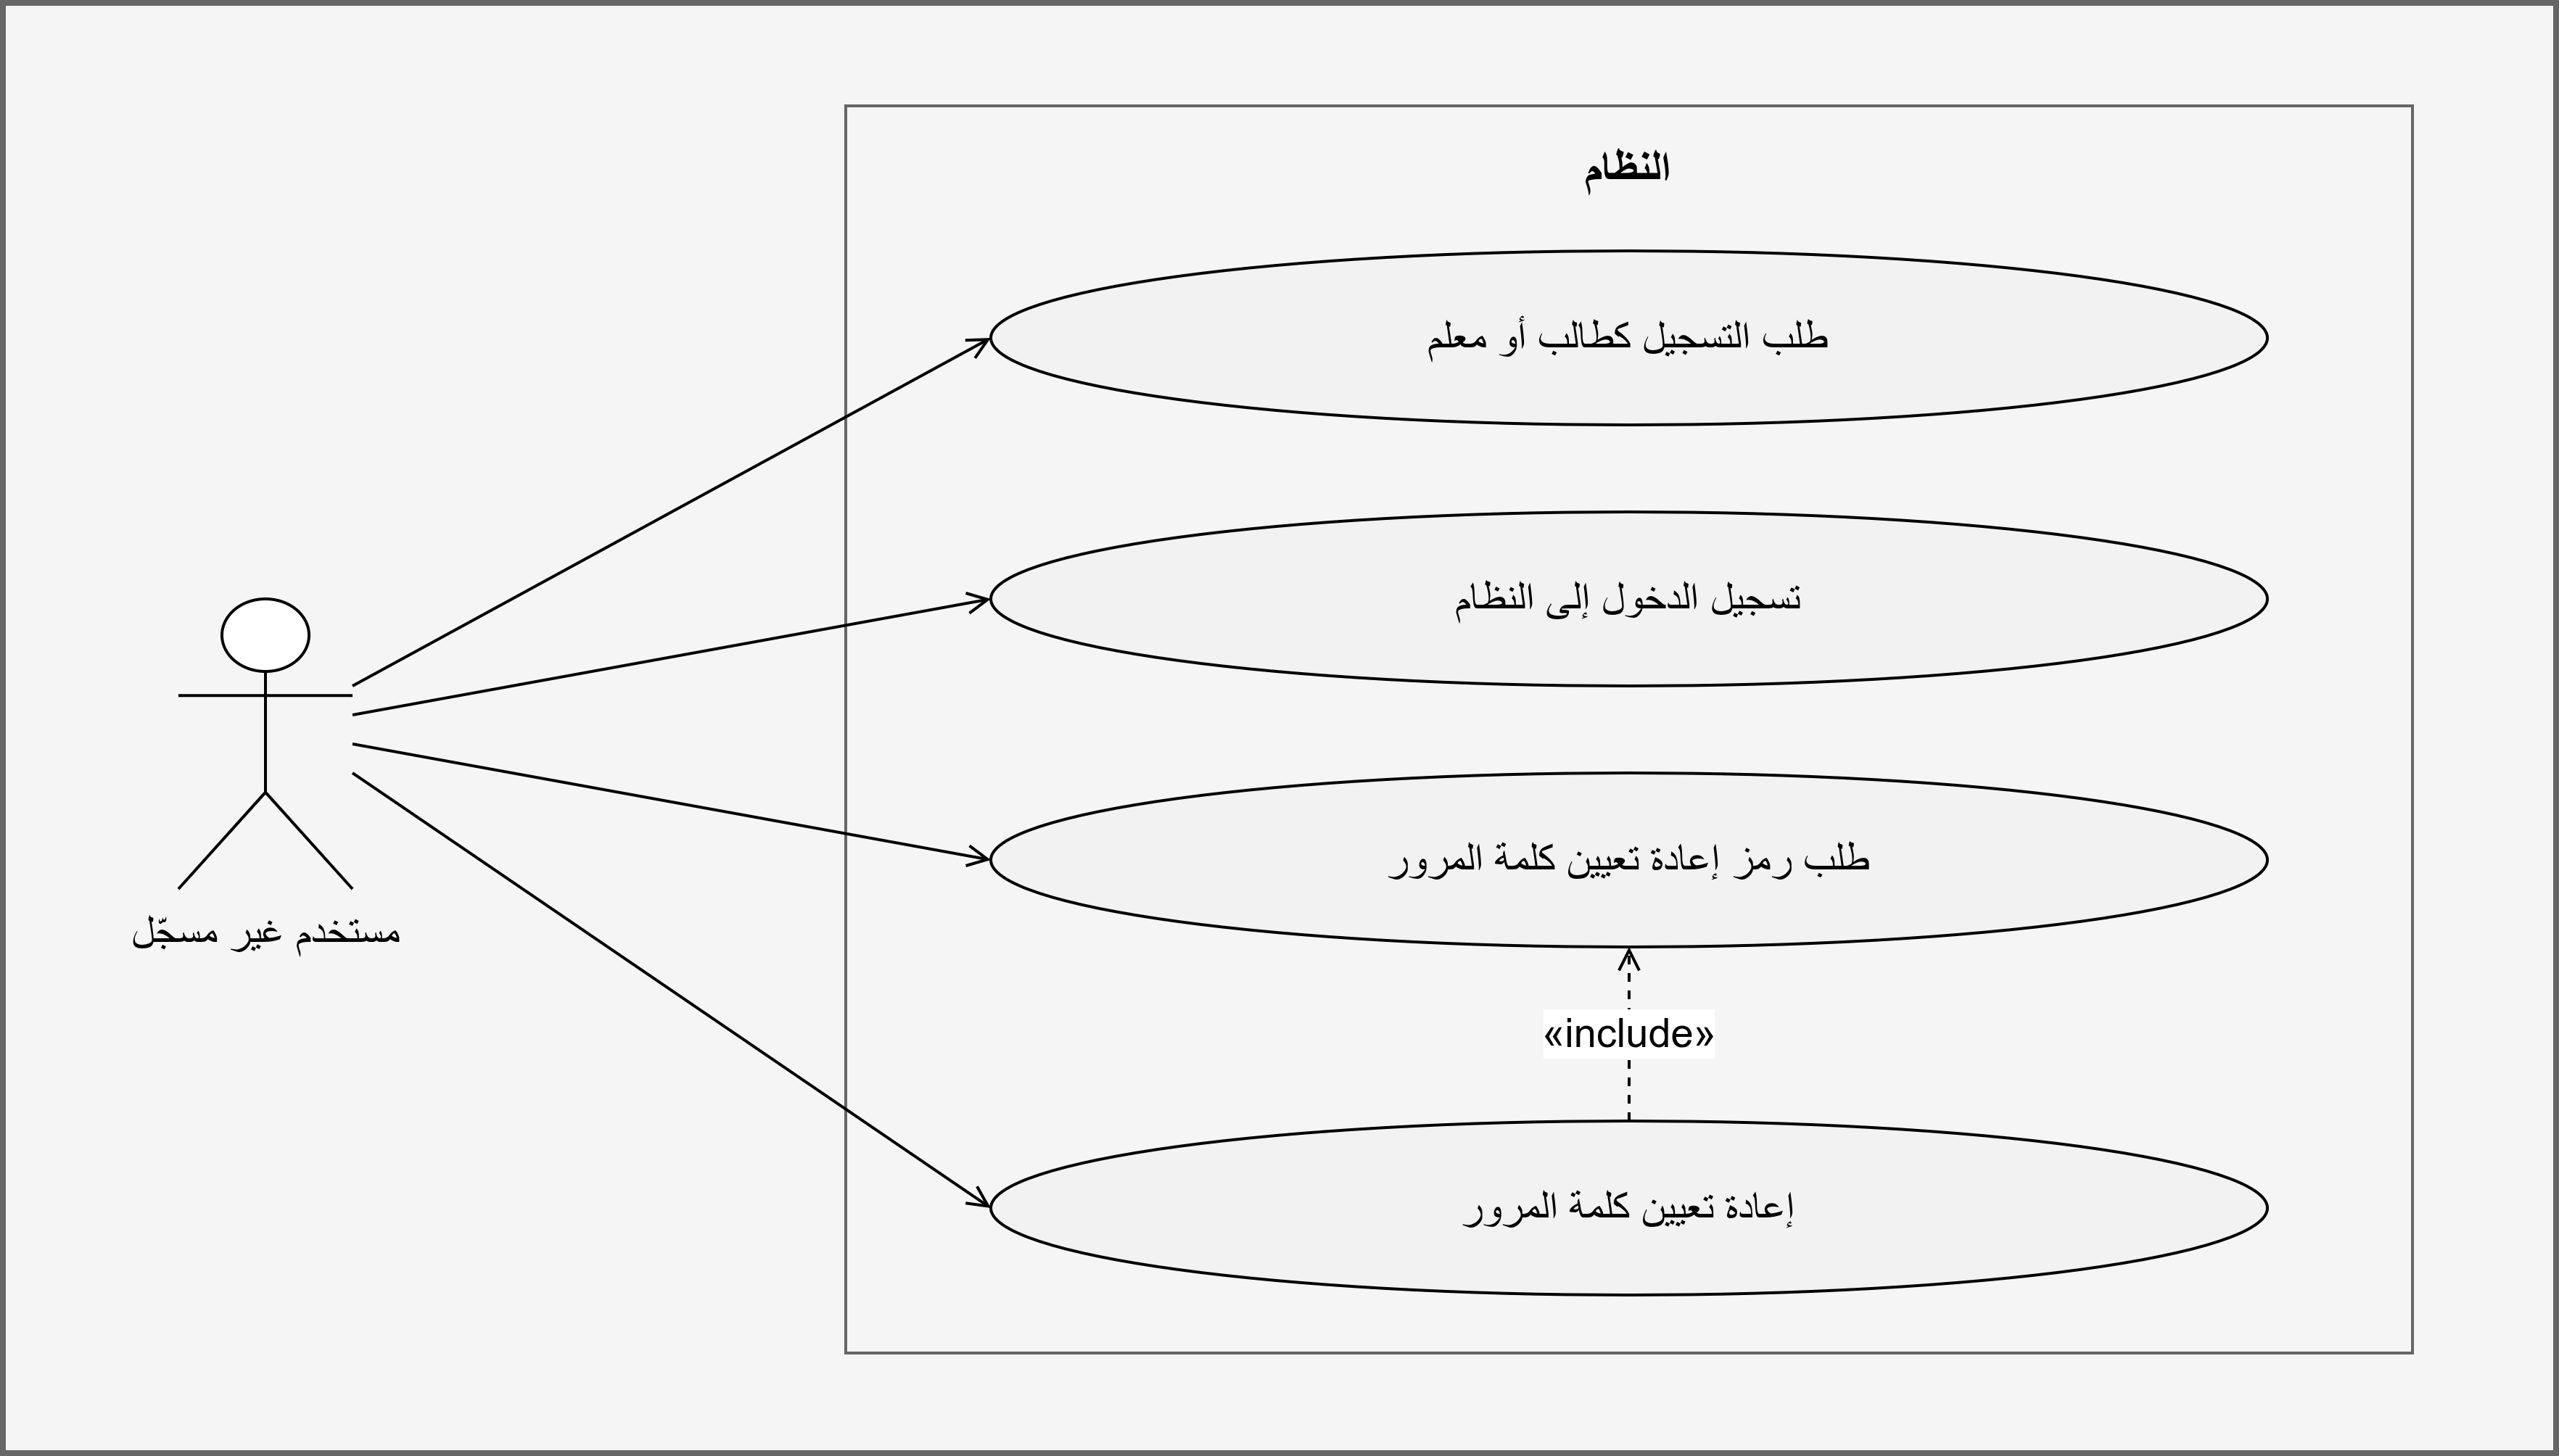
\includegraphics[width=\textwidth,height=0.8\textheight,keepaspectratio]{figures/uc-01-unregistered.png}
  \caption{حالات الاستخدام للمستخدم غير المسجّل: تبيّن ما يستطيع الزائر القيام به قبل امتلاك حساب، وهو محصور في التسجيل وتسجيل الدخول واستعادة كلمة المرور.}
  \label{fig:uc-01-unregistered}
\end{figure}

\clearpage
\subsection{حالات الاستخدام للمستخدمين المسجلين}

\begin{figure}[H]
  \centering
  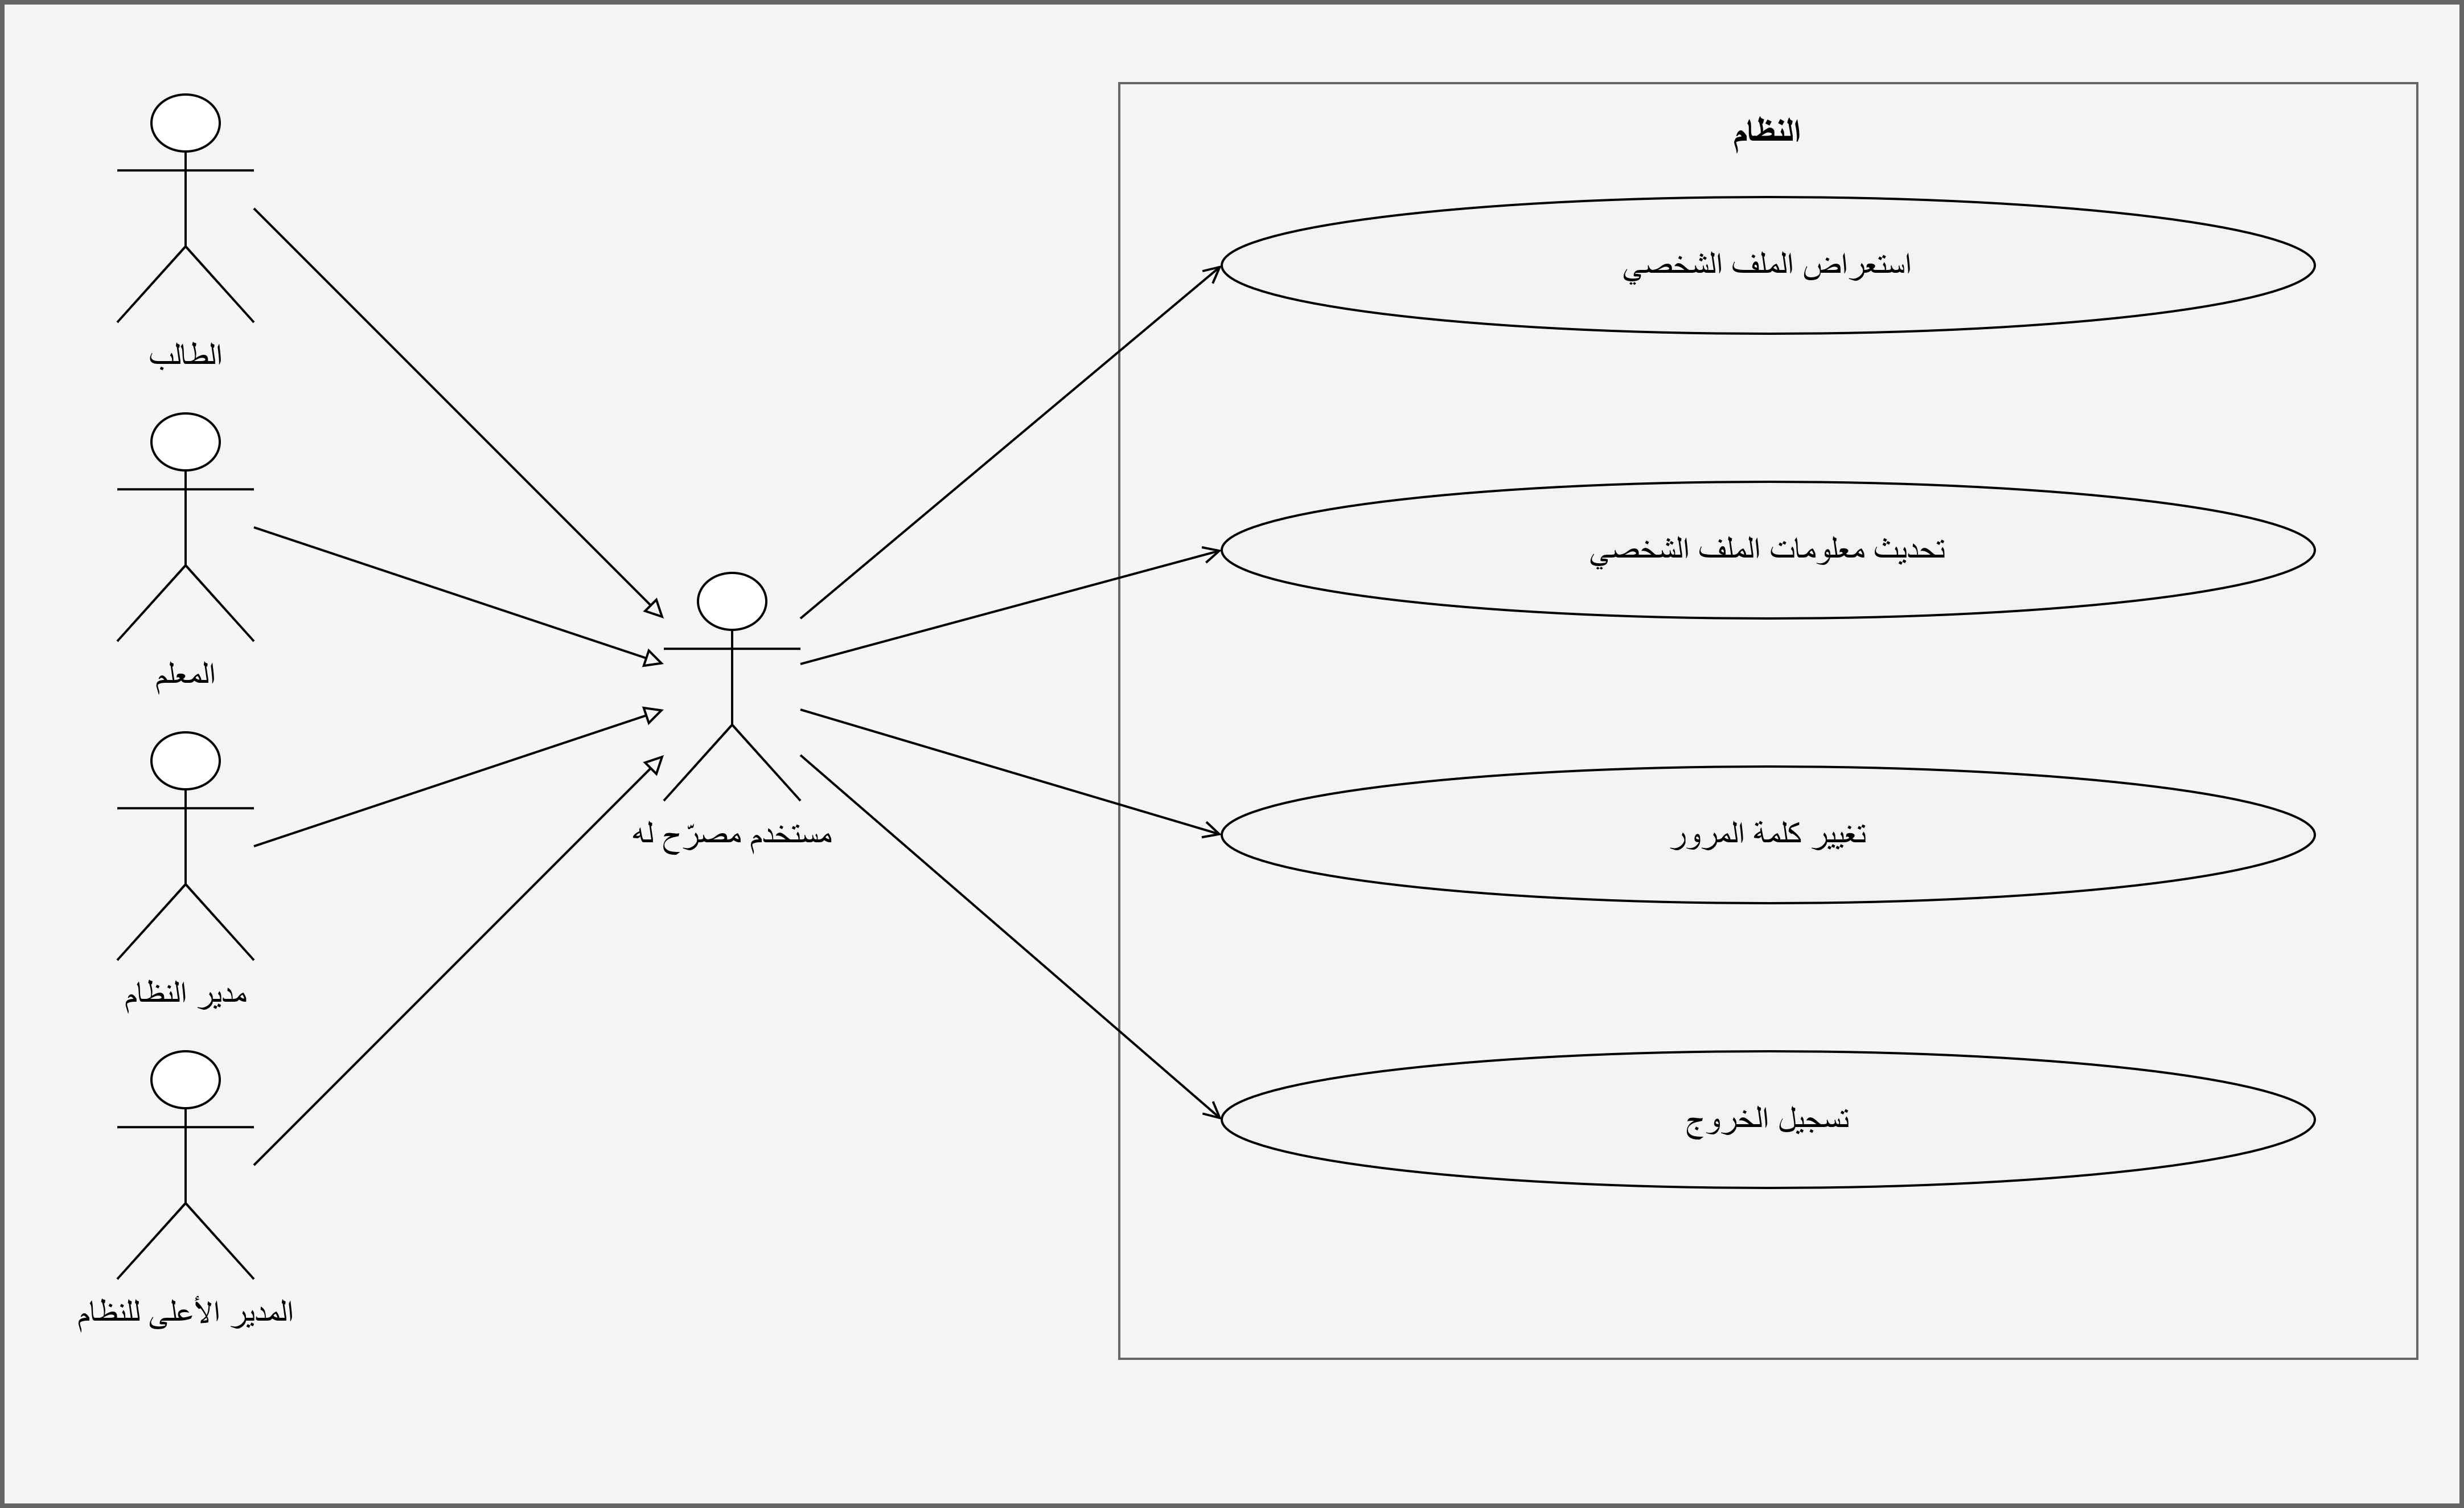
\includegraphics[width=\textwidth,height=0.8\textheight,keepaspectratio]{figures/uc-02-authorized.png}
  \caption{حالات الاستخدام المشتركة بين المستخدمين المسجّلين: العمليات المتاحة لكل صاحب حساب مهما كان دوره، وتتعلّق كلّها بإدارة ملفه الشخصي وجلسته.}
  \label{fig:uc-02-authorized}
\end{figure}

\clearpage
\subsection{حالات الاستخدام لمدير المظام الأعلى}

\begin{figure}[H]
  \centering
  \includegraphics[width=\textwidth,height=0.8\textheight,keepaspectratio]{figures/uc-03-super-admin.png}
  \caption{حالات الاستخدام لمدير النظام الأعلى: يتفرّد هذا الدور بإدارة حسابات المدراء وبالعمليات الهدّامة كحذف الفصول والجلسات ومخرجاتها.}
  \label{fig:uc-03-super-admin}
\end{figure}

\clearpage
\subsection{حالات الاستخدام لمدير النظام}

\begin{figure}[H]
  \centering
  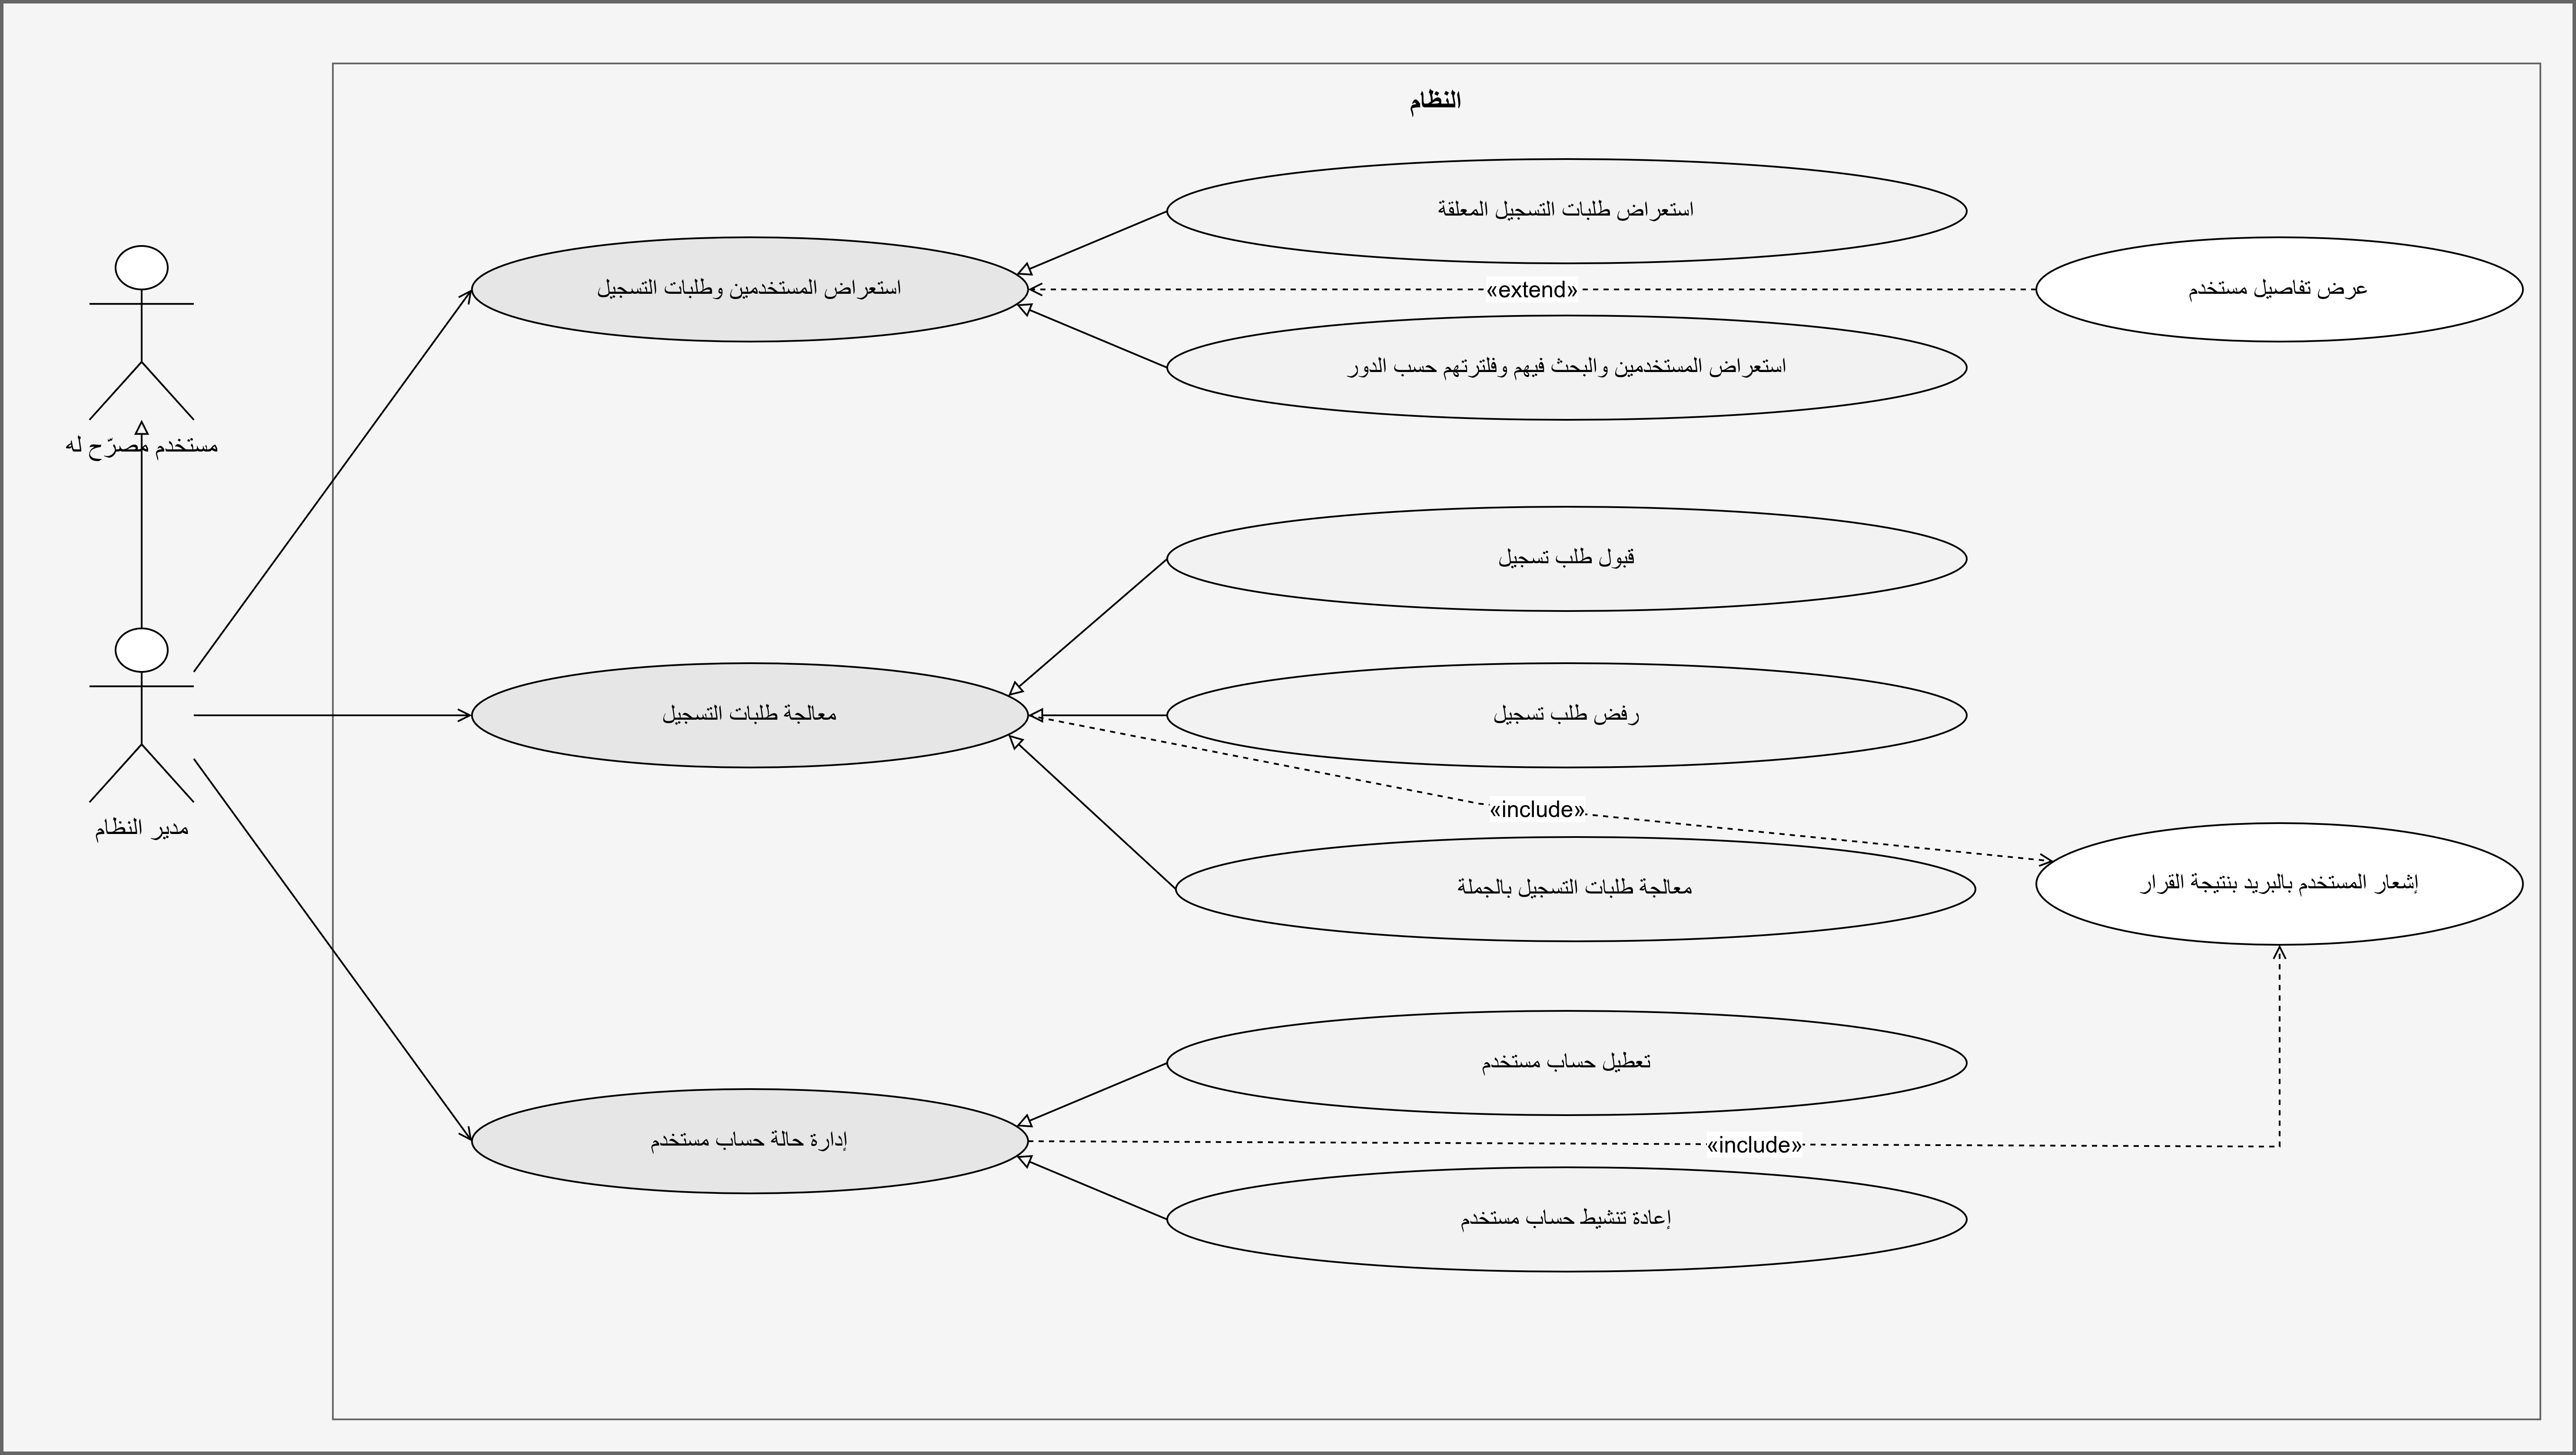
\includegraphics[width=\textwidth,height=0.8\textheight,keepaspectratio]{figures/uc-04-system-admin.png}
  \caption{حالات الاستخدام لمدير النظام: تتمحور حول معالجة طلبات التسجيل وإدارة حالات حسابات المستخدمين، دون صلاحية على حسابات المدراء أنفسهم.}
  \label{fig:uc-04-system-admin}
\end{figure}

\clearpage
\subsection{حالات الاستخدام للمعلم}

\begin{figure}[H]
  \centering
  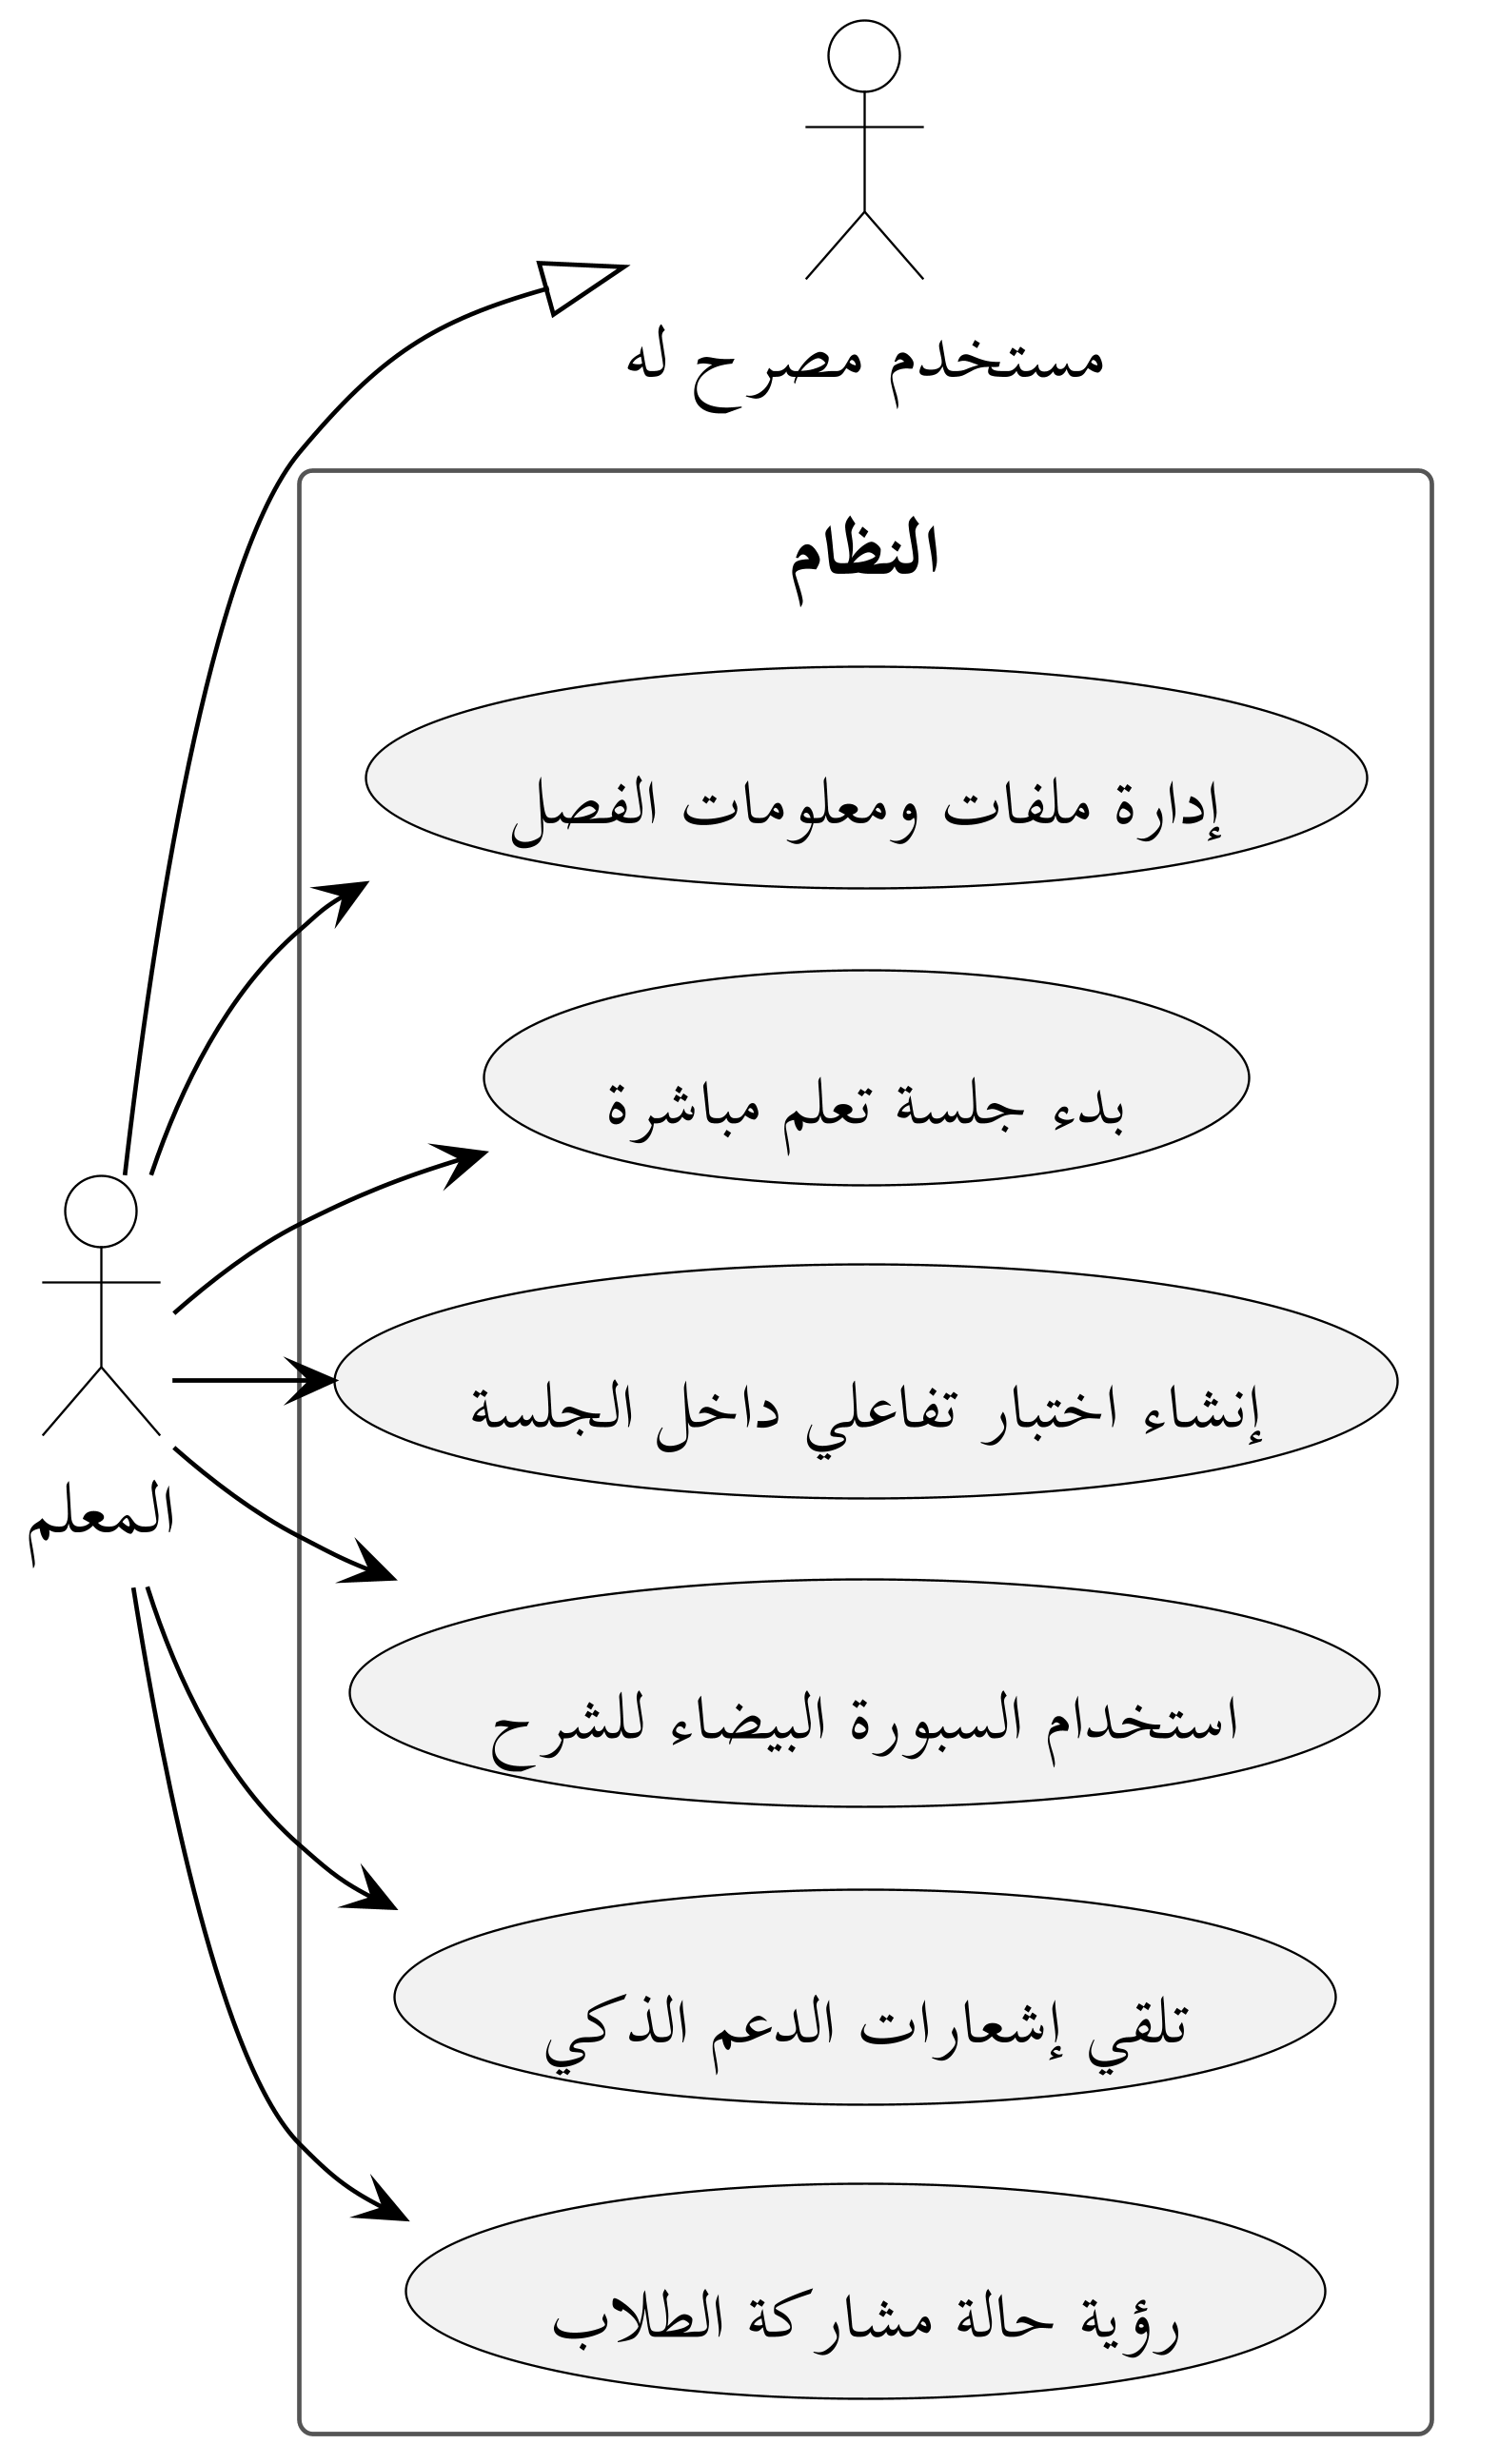
\includegraphics[width=\textwidth,height=0.8\textheight,keepaspectratio]{figures/uc-05-teacher.png}
  \caption{حالات الاستخدام للمعلم: تشمل إدارة فصوله وموادّه المرجعية، وإدارة دورة حياة الجلسة المباشرة من بدئها حتى إنهائها والاطّلاع على مخرجاتها.}
  \label{fig:uc-05-teacher}
\end{figure}

\clearpage
\subsection{حالات الاستخدام للطالب}

\begin{figure}[H]
  \centering
  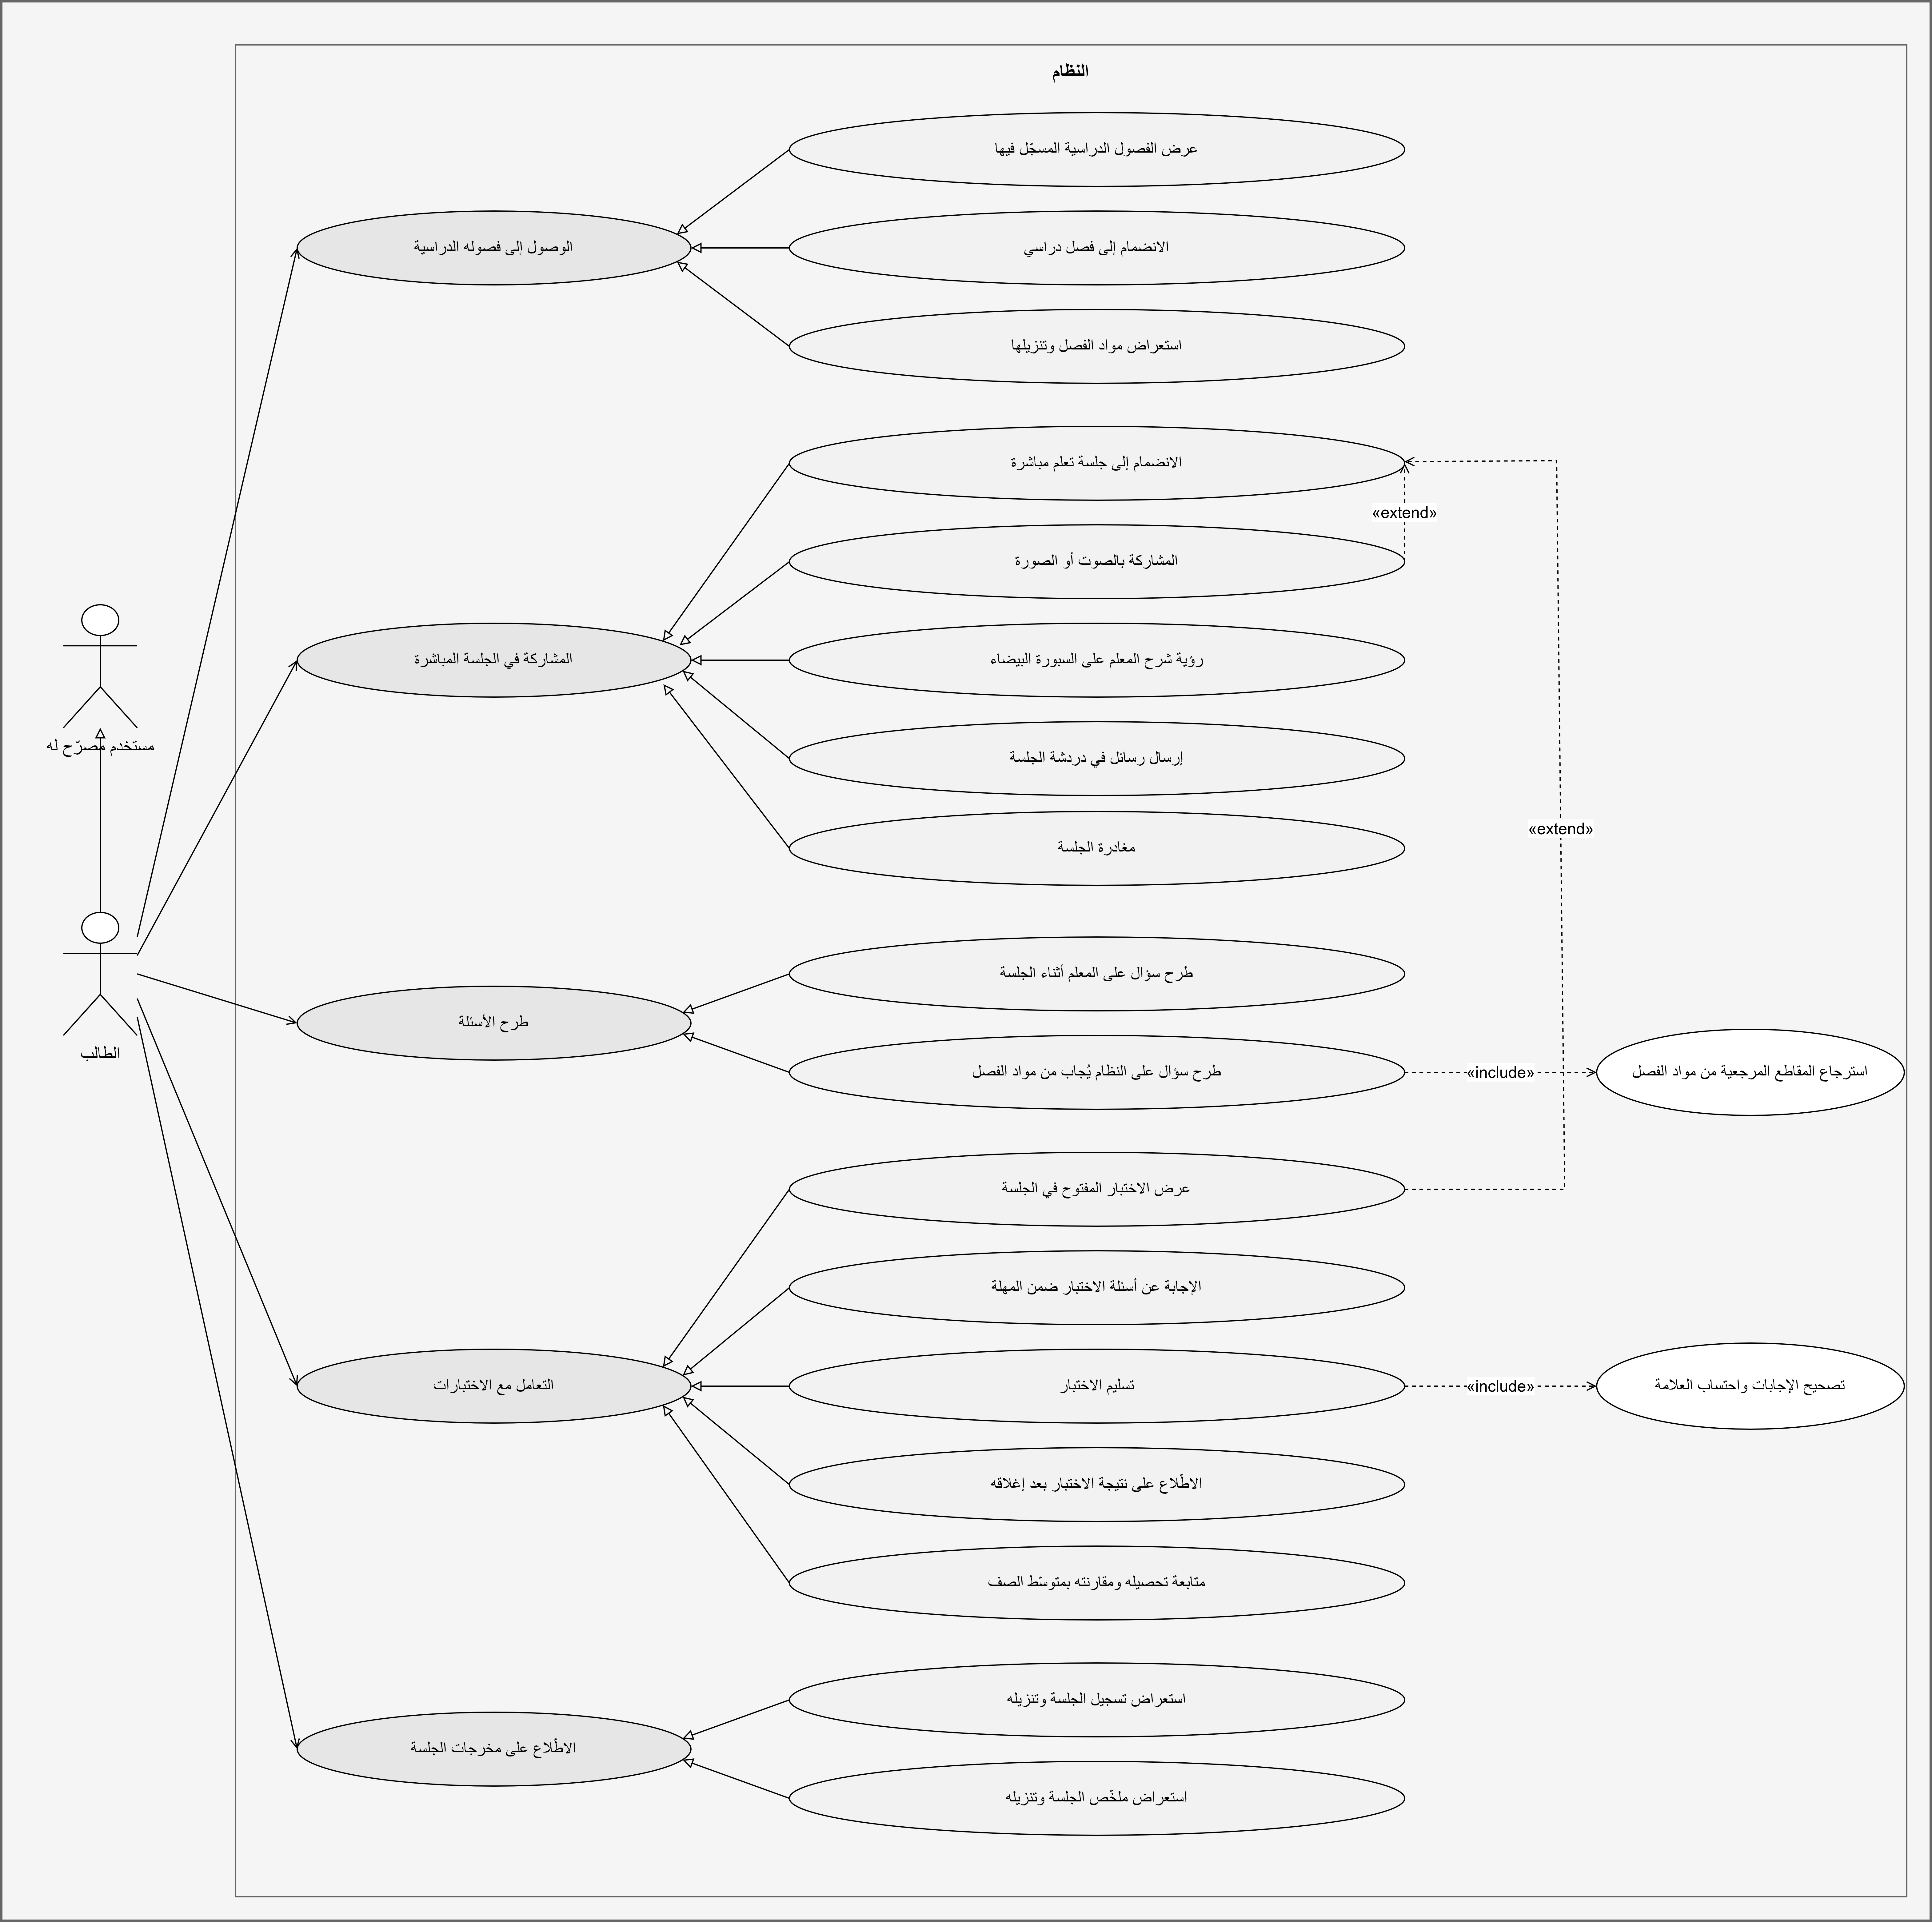
\includegraphics[width=\textwidth,height=0.8\textheight,keepaspectratio]{figures/uc-06-student.png}
  \caption{حالات الاستخدام للطالب: الانضمام إلى الجلسات المباشرة والتفاعل داخلها وطرح الأسئلة على النظام والاطّلاع على مخرجات الجلسة بعد انتهائها.}
  \label{fig:uc-06-student}
\end{figure}

\clearpage
\section{السرد النصي لحالات الاستخدام}

% ===========================================================================
% NARRATIVE SET — 7 use cases, ordered by system lifecycle, not by actor.
% Each narrative's preconditions are the previous one's postconditions.
% Fill them one at a time; find the empty ones with:
%   grep -n "TODO(uc-" chapters/04-requirements-analysis.tex
% Section 3 (SSDs) must mirror these seven in the same order.
% ===========================================================================

\subsection{تحضير المادة المرجعية}

\subsubsection{السرد النصي لحالة رفع ملف مرجعي إلى الفصل وفهرسته}
\label{subsubsec:uc-ingest}

\begin{enumerate}
  \item الاسم: رفع ملف مرجعي إلى الفصل الدراسي وفهرسته في قاعدة المعرفة
  \item الفاعل: المعلم
  \item الوصف: يرفع المعلم ملفًّا إلى فصله الدراسي، فيحفظه النظام ويعالج محتواه ويهيّئه للاسترجاع، حتى تصبح المادة مرجعًا يعتمد عليه في مساعدة المعلم وفي الإجابة عن أسئلة الطلاب.
  \item الشروط المسبقة
  \begin{enumerate}
    \item أن يكون المعلم مسجّلًا دخوله وأن يكون معلّم الفصل الدراسي المقصود.
    \item أن يكون الفصل الدراسي موجودًا.
  \end{enumerate}
  \item الشروط اللاحقة
  \begin{enumerate}
    \item أن يُحفظ الملف وأن تُسجَّل بياناته ضمن ملفات الفصل الدراسي.
    \item تصبح حالة فهرسة الملف ظاهرة للمعلم.
    \item أن يصبح محتوى الملف متاحًا للاسترجاع عند اكتمال الفهرسة بنجاح.
  \end{enumerate}
  \item السيناريو الرئيسي (المسار الناجح)
\end{enumerate}

\begin{ucflow}{السرد النصي لحالة الاستخدام «رفع ملف مرجعي إلى الفصل وفهرسته»: يعرض خطوات المسار الرئيسي مقابلةً بين ما يقوم به الفاعل وما يستجيب به النظام في كل خطوة.}{المعلم}
    1. يطلب المعلم رفع ملفات لفصله الدراسي. &  \\ \hline
     & 2. يعرض النظام حدود الرفع من حجم أقصى وصيغ مقبولة، قبل أن يختار المعلم ملفًّا. \\ \hline
    3. يختار المعلم الملف ويؤكّد رفعه. &  \\ \hline
     & 4. يتحقّق النظام من هوية الفاعل ومن كونه معلّم هذا الفصل. \\ \hline
     & 5. يتحقّق النظام من أنّ الملف غير فارغ وأنّ حجمه ضمن الحدّ الأقصى، ومن أنّ صيغته مقبولة اعتمادًا على نوع محتواه أو امتداده. \\ \hline
     & 6. يحفظ النظام الملف ضمن الفصل الدراسي بمعرّف فريد يمنع تضارب الأسماء المتشابهة. \\ \hline
     & 7. يسجّل النظام بيانات الملف من اسم ونوع وحجم ضمن ملفات الفصل. \\ \hline
     & 8. يُعلم النظام المعلم بنجاح الرفع ويُظهر الملف في قائمة ملفات الفصل مبيّنًا حالة فهرسته. \\ \hline
     & 9. يستخرج النظام نصّ الملف بحسب صيغته، ويستخرجه كذلك من صفحاته المصوَّرة التي لا نصّ فيها. \\ \hline
     & 10. يقسّم النظام النصّ المستخرج إلى مقاطع ويهيّئها للاسترجاع، فتصبح حالة الملف «مفهرَس». \\ \hline
\end{ucflow}

\begin{enumerate}
  \item المسارات البديلة (الاستثناءات)
  \begin{enumerate}
    \item \textbf{4: اذا كان الفاعل ليس معلّم الفصل يرفض النظام الطلب. }
    \item \textbf{5: اذا كان حجم الملف يتجاوز الحدّ الأقصى يرفض النظام الطلب. }
    \item \textbf{5: اذا كان الملف فارغًا يرفض النظام الرفع ويُعلم المعلم بالحدّ المسموح. }
    \item \textbf{5: اذا كانت صيغة الملف غير مقبولة يرفض النظام الرفع ويعرض للمعلم الصيغ المقبولة. }
    \item \textbf{9: اذا كان محتوى الملف مطابقًا لآخر فهرسة ناجحة تُعدّ الفهرسة مكتملة من غير إعادة معالجته، لأنّ ما فُهرس منه سابقًا ما يزال صالحًا. }
    \item \textbf{9: اذا لم يُستخرج من الملف أيّ نصّ يُعلم النظام المعلم بتعذّر فهرسته مع بيان السبب، ولا يَعُدّه مفهرسًا. }
    \item \textbf{10: اذا تعذّرت فهرسة الملف يبقى رفعه ناجحًا، ويبقى الملف غير مفهرس إلى أن تطلب إعاد الفهرسة يدويًّا. }
  \end{enumerate}
\end{enumerate}

\subsection{جلسة التعلم المباشرة}

\subsubsection{السرد النصي لحالة الشرح على السبورة والتفاعل داخل الجلسة}
\label{subsubsec:uc-whiteboard}

\begin{enumerate}
  \item الاسم: الشرح على السبورة البيضاء والتفاعل داخل جلسة التعلم المباشرة
  \item الفاعل: المعلم فاعلًا رئيسًا، والطالب فاعلًا مشاركًا
  \item الوصف: يشرح المعلم على سبورة بيضاء تعلو صورة الجلسة، فيرى الطلاب ما يرسمه المعلم، ويتفاعلون معه في أثناء ذلك بالدردشة وبطرح الأسئلة، ويضبط المعلم ما يُسمح لهم بمشاركته من صوت أو صورة.
  \item الشروط المسبقة
  \begin{enumerate}
    \item أن تكون جلسة التعلم المباشرة جارية وأن يكون المعلم متّصلًا بها.
    \item أن يكون الطلاب المشاركون أعضاء في الفصل الدراسي وقد انضمّوا إلى الجلسة.
  \end{enumerate}
  \item الشروط اللاحقة
  \begin{enumerate}
    \item أن يرى المشاركون جميعًا السبورة نفسها بما عليها.
    \item أن تُحفظ رسائل الدردشة وأسئلة الجلسة وإجاباتها ضمن سجل الجلسة.
    \item أن يسري ما قرّره المعلم في مشاركة الطلاب للصوت والصورة على الجلسة كلّها.
  \end{enumerate}
  \item السيناريو الرئيسي (المسار الناجح)
\end{enumerate}

\begin{ucflow}{السرد النصي لحالة الاستخدام «الشرح على السبورة والتفاعل داخل الجلسة»: يعرض خطوات المسار  أوّلًا بأوّلالرئيسي مقابلةً بين ما يقوم به الفاعل وما يستجيب به النظام في كل خطوة.}{المعلم والطالب}
    1. يُفعّل المعلم السبورة البيضاء، مختارًا الرسم فوق ما يعرضه على الطلاب أو على سطح فارغ. &  \\ \hline
     & 2. يعرض النظام سطح الرسم مضبوطًا على أبعاد الصورة المعروضة، ويتيح للمعلم أدوات القلم والأشكال والنص والمؤشّر الضوئي والممحاة. \\ \hline
    3. يرسم المعلم على السبورة أو يكتب عليها في أثناء شرحه. &  \\ \hline
     & 4. يُظهر النظام ما يرسمه المعلم على شاشات الطلاب، في موضعه نفسه من الصورة مهما اختلفت أحجام شاشاتهم. \\ \hline
    5. يجمّد المعلم الصورة ليشرح على لقطة بعينها، ثمّ يرفع التجميد. &  \\ \hline
     & 6. يثبّت النظام اللقطة نفسها عند الطلاب جميعًا، ثمّ يعيدهم إلى البثّ المباشر عند رفع التجميد. \\ \hline
     & 7. يزوّد النظام كلّ طالب ينضم بعد بدء الشرح بما رُسم على السبورة قبل انضمامه، فيرى ما يراه بقيّة الصف. \\ \hline
    8. يتراجع المعلم عن آخر ما رسمه، أو يخفي السبورة، أو يمسحها كلّها. &  \\ \hline
     & 9. يحدّث النظام السبورة عند المشاركين جميعًا بحيث تبقى واحدة عندهم. \\ \hline
    10. يرسل أحد المشاركين رسالة في دردشة الجلسة. &  \\ \hline
     & 11. يوزّع النظام الرسالة على المشاركين في الجلسة ويحفظها في سجل دردشتها. \\ \hline
    12. يطرح الطالب سؤالًا على المعلم في أثناء الشرح. &  \\ \hline
     & 13. يعرض النظام السؤال للمعلم ضمن أسئلة الجلسة. \\ \hline
    14. يجيب المعلم عن السؤال. &  \\ \hline
     & 15. يعرض النظام الإجابة مقترنة بسؤالها للمشاركين. \\ \hline
    16. يسمح المعلم للطلاب بمشاركة الصوت أو الصورة، أو يمنعهم منها. &  \\ \hline
     & 17. يطبّق النظام قرار المعلم على الجلسة ويُعلم المشاركين جميعًا بما صار مسموحًا لهم. \\ \hline
\end{ucflow}

\begin{enumerate}
  \item المسارات البديلة (الاستثناءات)
  \begin{enumerate}
    \item \textbf{2: اذا كان الفاعل ليس معلّم الجلسة لا يتيح له النظام الرسم على السبورة، ويكتفي بعرضها عليه. }
    \item \textbf{4: اذا انقطع اتّصال طالب في أثناء الرسم يستدرك النظام ما فاته عند عودته، فتعود سبورته مطابقة لسبورة المعلم. }
    \item \textbf{4: اذا تعذّر إيصال ما رُسم لحظتَه لا يقطع النظام الشرح، وتُصحَّح السبورة في أوّل مزامنة تالية. }
    \item \textbf{7: اذا كان المعلم هو من أُعيد اتّصاله بالجلسة يعيد النظام مزامنة السبورة عند المشاركين جميعًا، حتى لا تبقى عندهم رسوم لم يعد المعلم قادرًا على محوها. }
    \item \textbf{11: اذا كانت الرسالة فارغة يهملها النظام ولا يوزّعها. }
    \item \textbf{16: اذا كان الفاعل ليس معلّم الجلسة يرفض النظام تغيير ما يُسمح به للطلاب. }
    \item \textbf{17: اذا منع المعلم مشاركة الصوت أو الصورة يوقف النظام ما هو منشور منهما ويمنع أيّ مشاركة جديدة إلى أن يُعاد السماح.}
  \end{enumerate}
\end{enumerate}

\subsubsection{السرد النصي لحالة تحليل شرح المعلم وإشعار المساعد المباشر}
\label{subsubsec:uc-drift}
% TODO(uc-3)

\subsubsection{السرد النصي لحالة طرح سؤال يُجاب من مواد الفصل}
\label{subsubsec:uc-qa}
% TODO(uc-4)

\subsection{الاختبارات داخل الجلسة}

\subsubsection{السرد النصي لحالة إنشاء مسودة اختبار وتعديلها ونشرها}
\label{subsubsec:uc-quiz-compose}
% TODO(uc-5)

\subsubsection{السرد النصي لحالة الإجابة عن الاختبار وتسليمه وتصحيحه}
\label{subsubsec:uc-quiz-answer}
% TODO(uc-6)

\subsection{مخرجات الجلسة}

\subsubsection{السرد النصي لحالة إنهاء الجلسة وتوليد الملخّص}
\label{subsubsec:uc-session-end}
% TODO(uc-7)

\section{مخططات تسلسل النظام}

\subsection{مخطط تسلسل النظام لحالات استخدام مدير النظام الاعلى}

\subsubsection{تدفّق تسجيل دخول المدير الأعلى}
\label{subsubsec:flow-super-admin-login}

يجري تسجيل دخول المدير الأعلى على مرحلتين يبيّنهما الشكلان~\ref{fig:flow-01a} و\ref{fig:flow-01b}.

\begin{figure}[htbp]
  \centering
  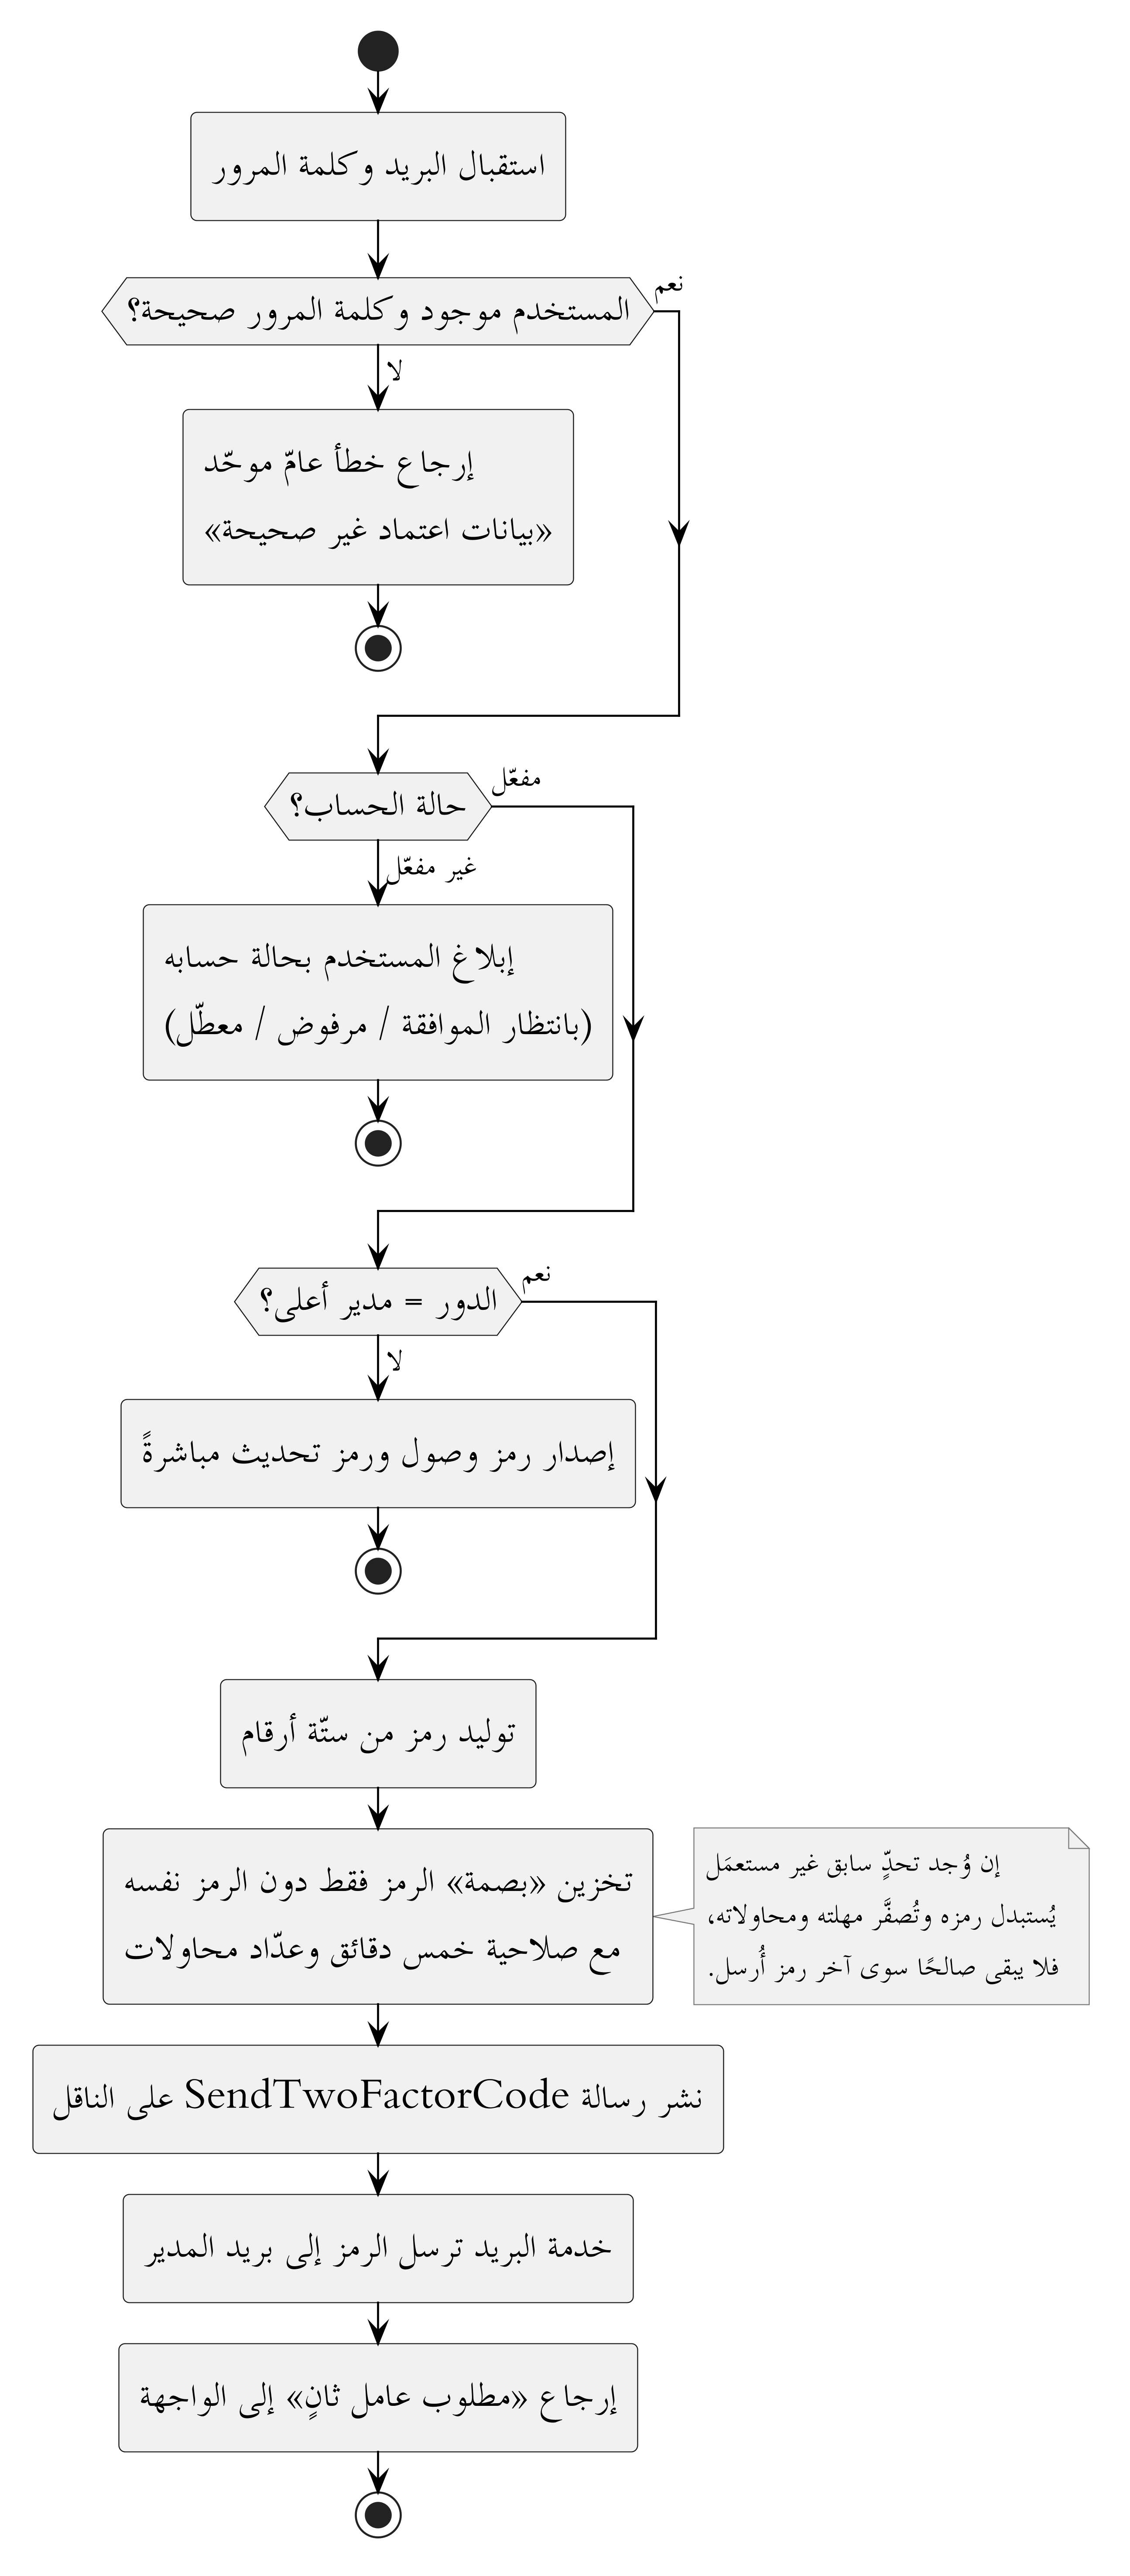
\includegraphics[width=\textwidth,height=0.8\textheight,keepaspectratio]{figures/flow-01a-two-factor-challenge.png}
  \caption{تدفّق المرحلة الأولى من تسجيل دخول المدير الأعلى: التحقّق من الاعتماد وإصدار التحدّي.}
  \label{fig:flow-01a}
\end{figure}

\begin{figure}[htbp]
  \centering
  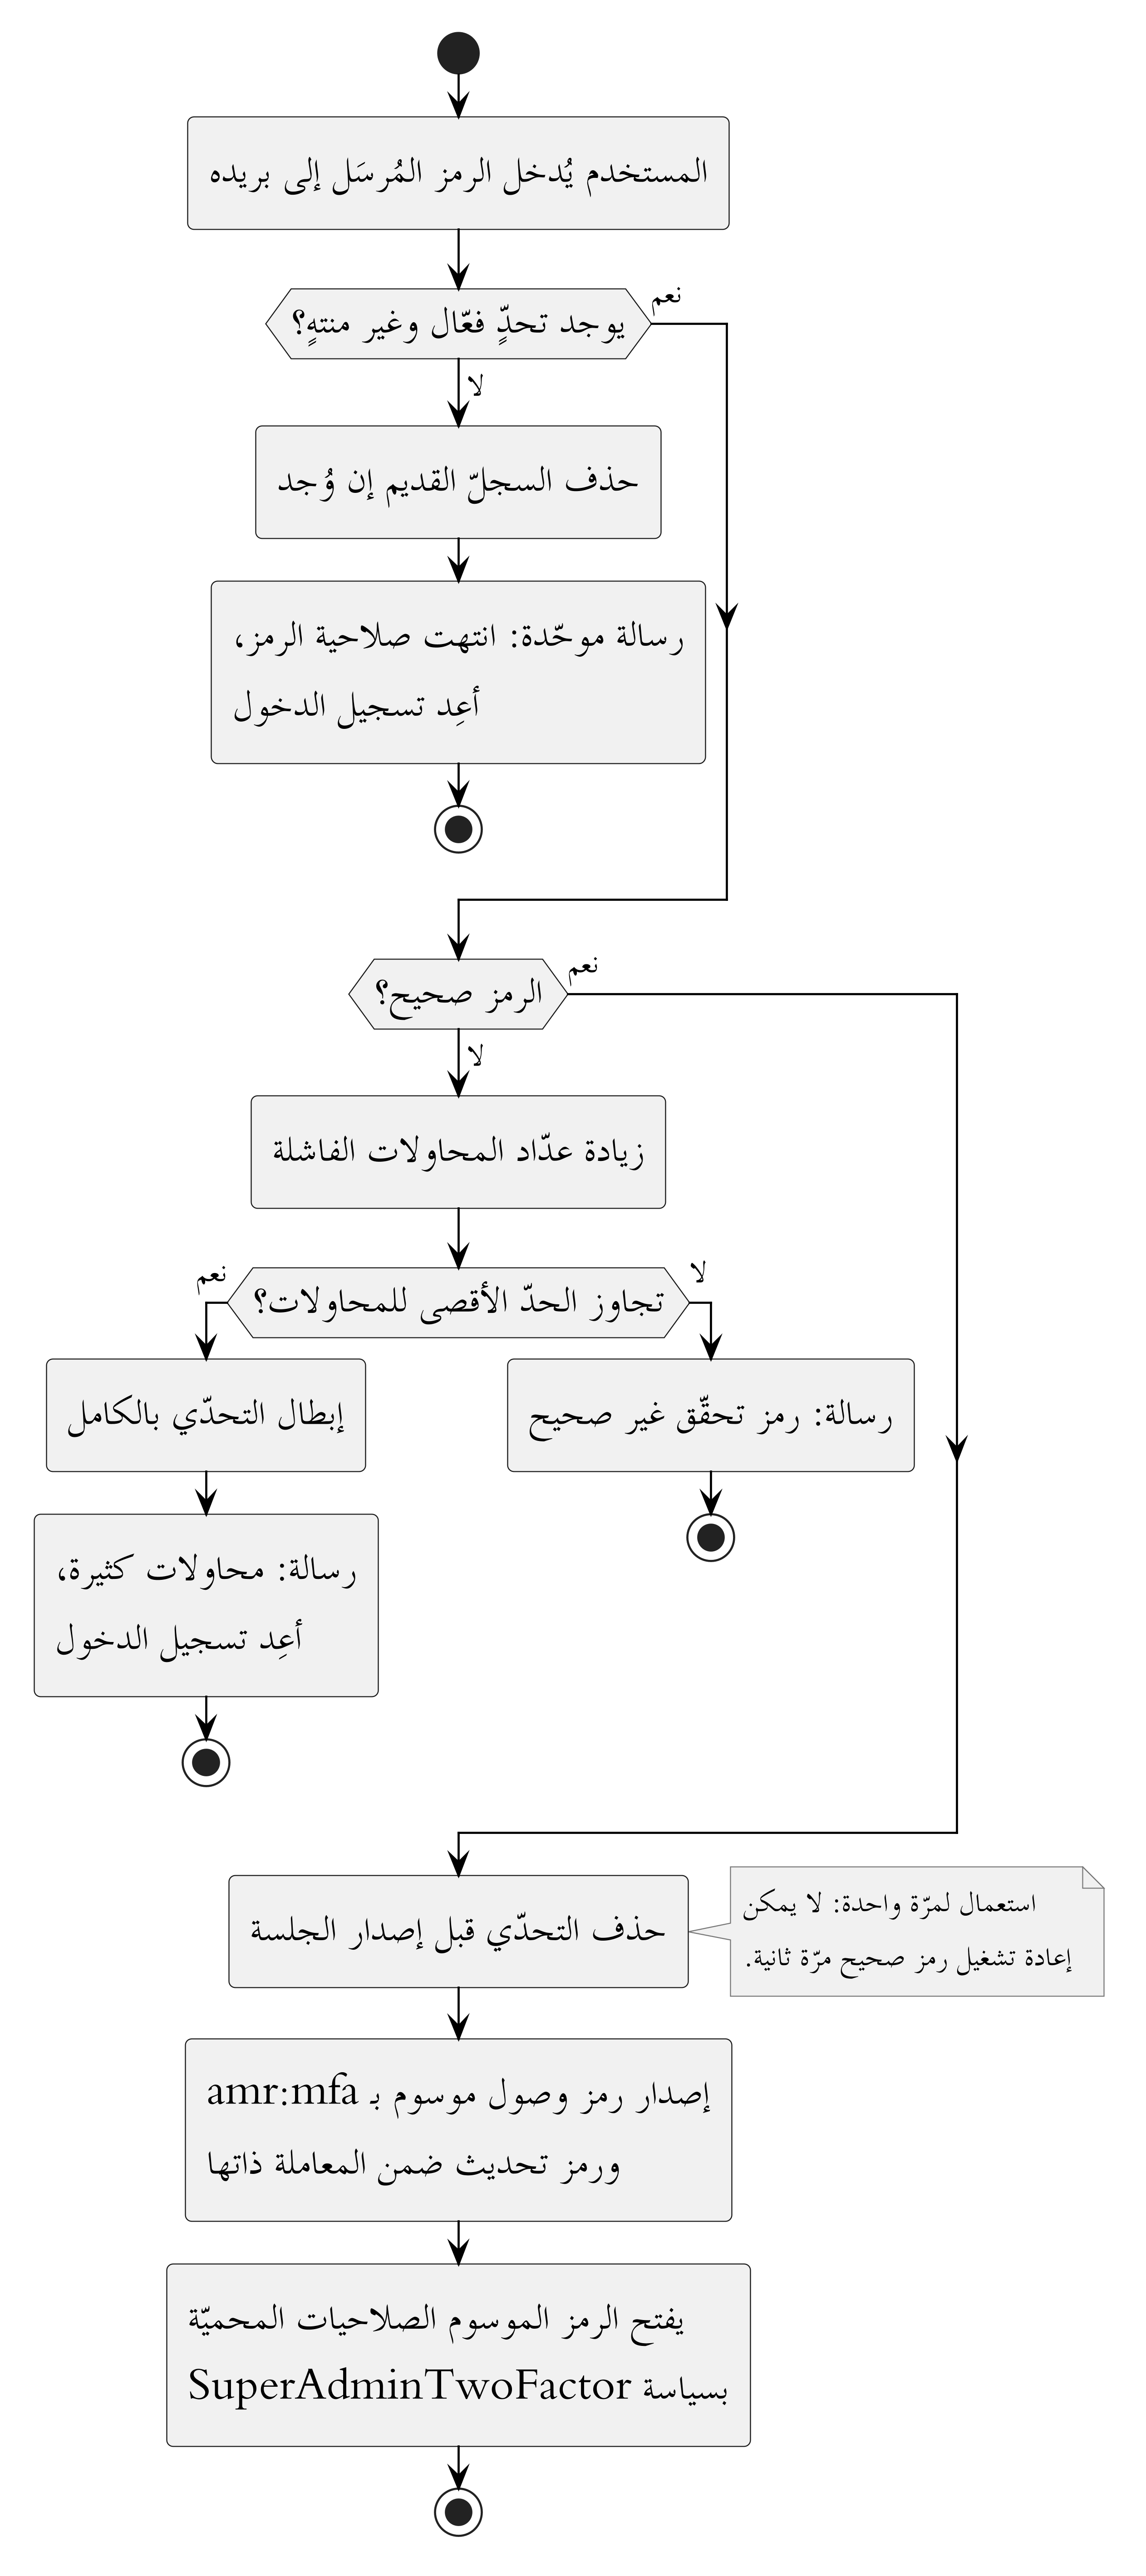
\includegraphics[width=\textwidth,height=0.8\textheight,keepaspectratio]{figures/flow-01b-two-factor-verify.png}
  \caption{تدفّق المرحلة الثانية من تسجيل دخول المدير الأعلى: التحقّق من الرمز وإصدار الجلسة.}
  \label{fig:flow-01b}
\end{figure}

\noindent يجري تسجيل دخول المدير الأعلى على مرحلتين منفصلتين بطلبين مستقلّين، بينهما تحدٍّ قصير العمر وحيد الاستعمال. وهو أكثر منطق خدمة إدارة المستخدمين تركيبًا. وقد بُيّنت مرحلتاه في الشكلين~\ref{fig:flow-01a} و\ref{fig:flow-01b}.

ويقوم هذا التدفّق على ثلاثة ضوابط أمنية:

\begin{enumerate}
  \item \textbf{توحيد رسائل الفشل}: يُرجِع النظام رسالة فشل عامّة واحدة، سواء أكان البريد غير مسجَّل أم كانت كلمة المرور خاطئة. ويمنع ذلك استعمال نقطة النهاية للكشف عن العناوين المسجَّلة في النظام.
  \item \textbf{تخزين البصمة لا الرمز}: تُحفَظ بصمة رمز العامل الثاني لا الرمز نفسه، فلا يمنح تسريب قاعدة البيانات رمزًا صالحًا للاستعمال.
  \item \textbf{حذف التحدّي قبل إصدار الجلسة}: يُحذَف سجلّ التحدّي قبل توليد الرمز، فلا يمكن إعادة استعمال رمز صحيح مرّةً ثانية.
\end{enumerate}

ويُوسَم رمز الوصول الناتج بالادّعاء \en{amr:mfa}، وهو ما تشترطه السياسة \en{SuperAdminTwoFactor} لفتح الصلاحيات الأشدّ حساسية.

\subsubsection{مخطط تسلسل النظام لحالة استعراض الجلسات والبحث فيها}

\begin{figure}[htbp]
  \centering
  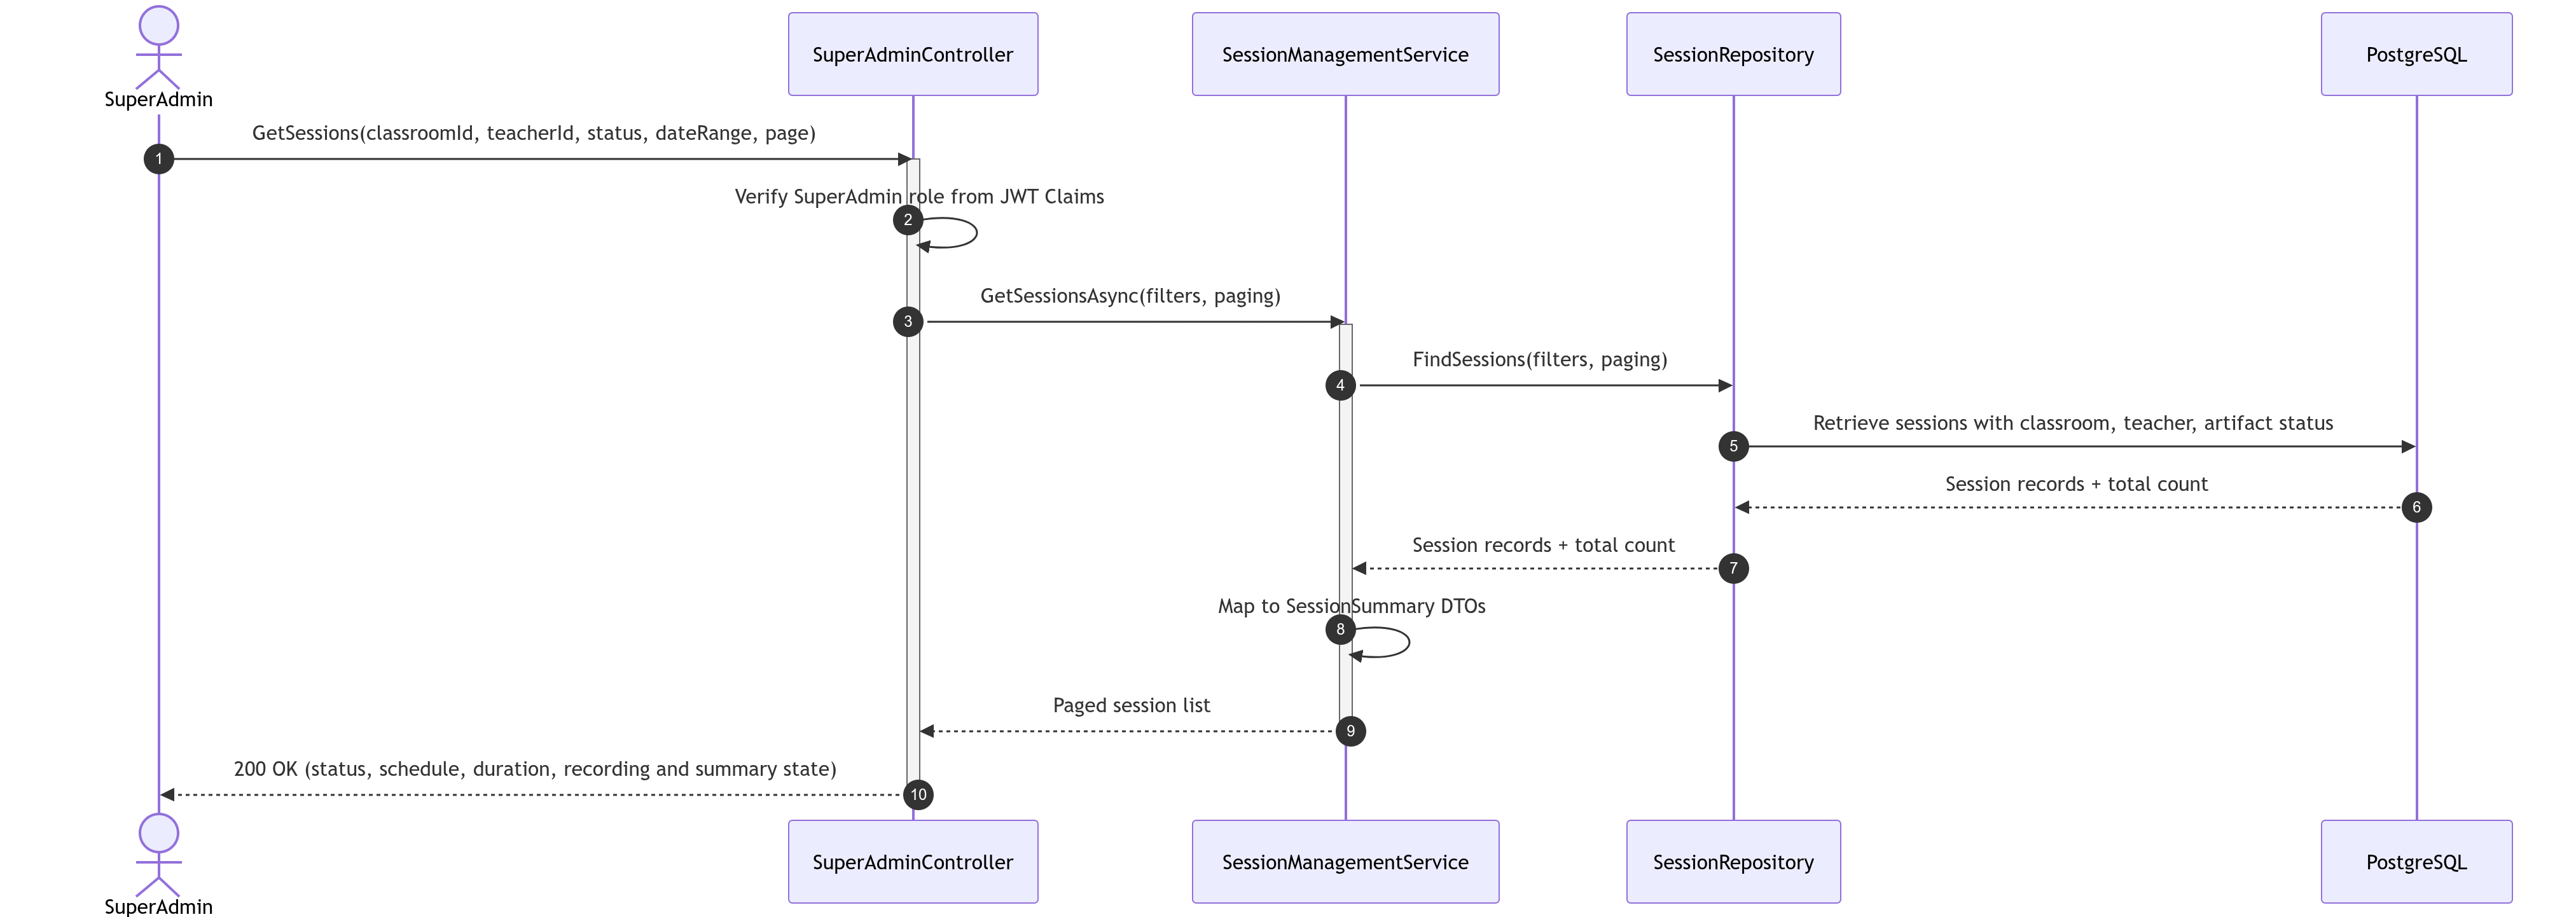
\includegraphics[width=\textwidth,height=0.8\textheight,keepaspectratio]{figures/image25.png}
  \caption{مخطط تسلسل النظام لحالة «استعراض الجلسات والبحث فيها»: يوضّح الرسائل المتبادلة بين الفاعل والنظام بوصفه صندوقًا أسود، أي دون إظهار الخدمات الداخلية التي تنفّذها.}
  \label{fig:image25}
\end{figure}

\subsubsection{مخطط تسلسل النظام لحالة عرض الجلسات الحية النشطة}

\begin{figure}[htbp]
  \centering
  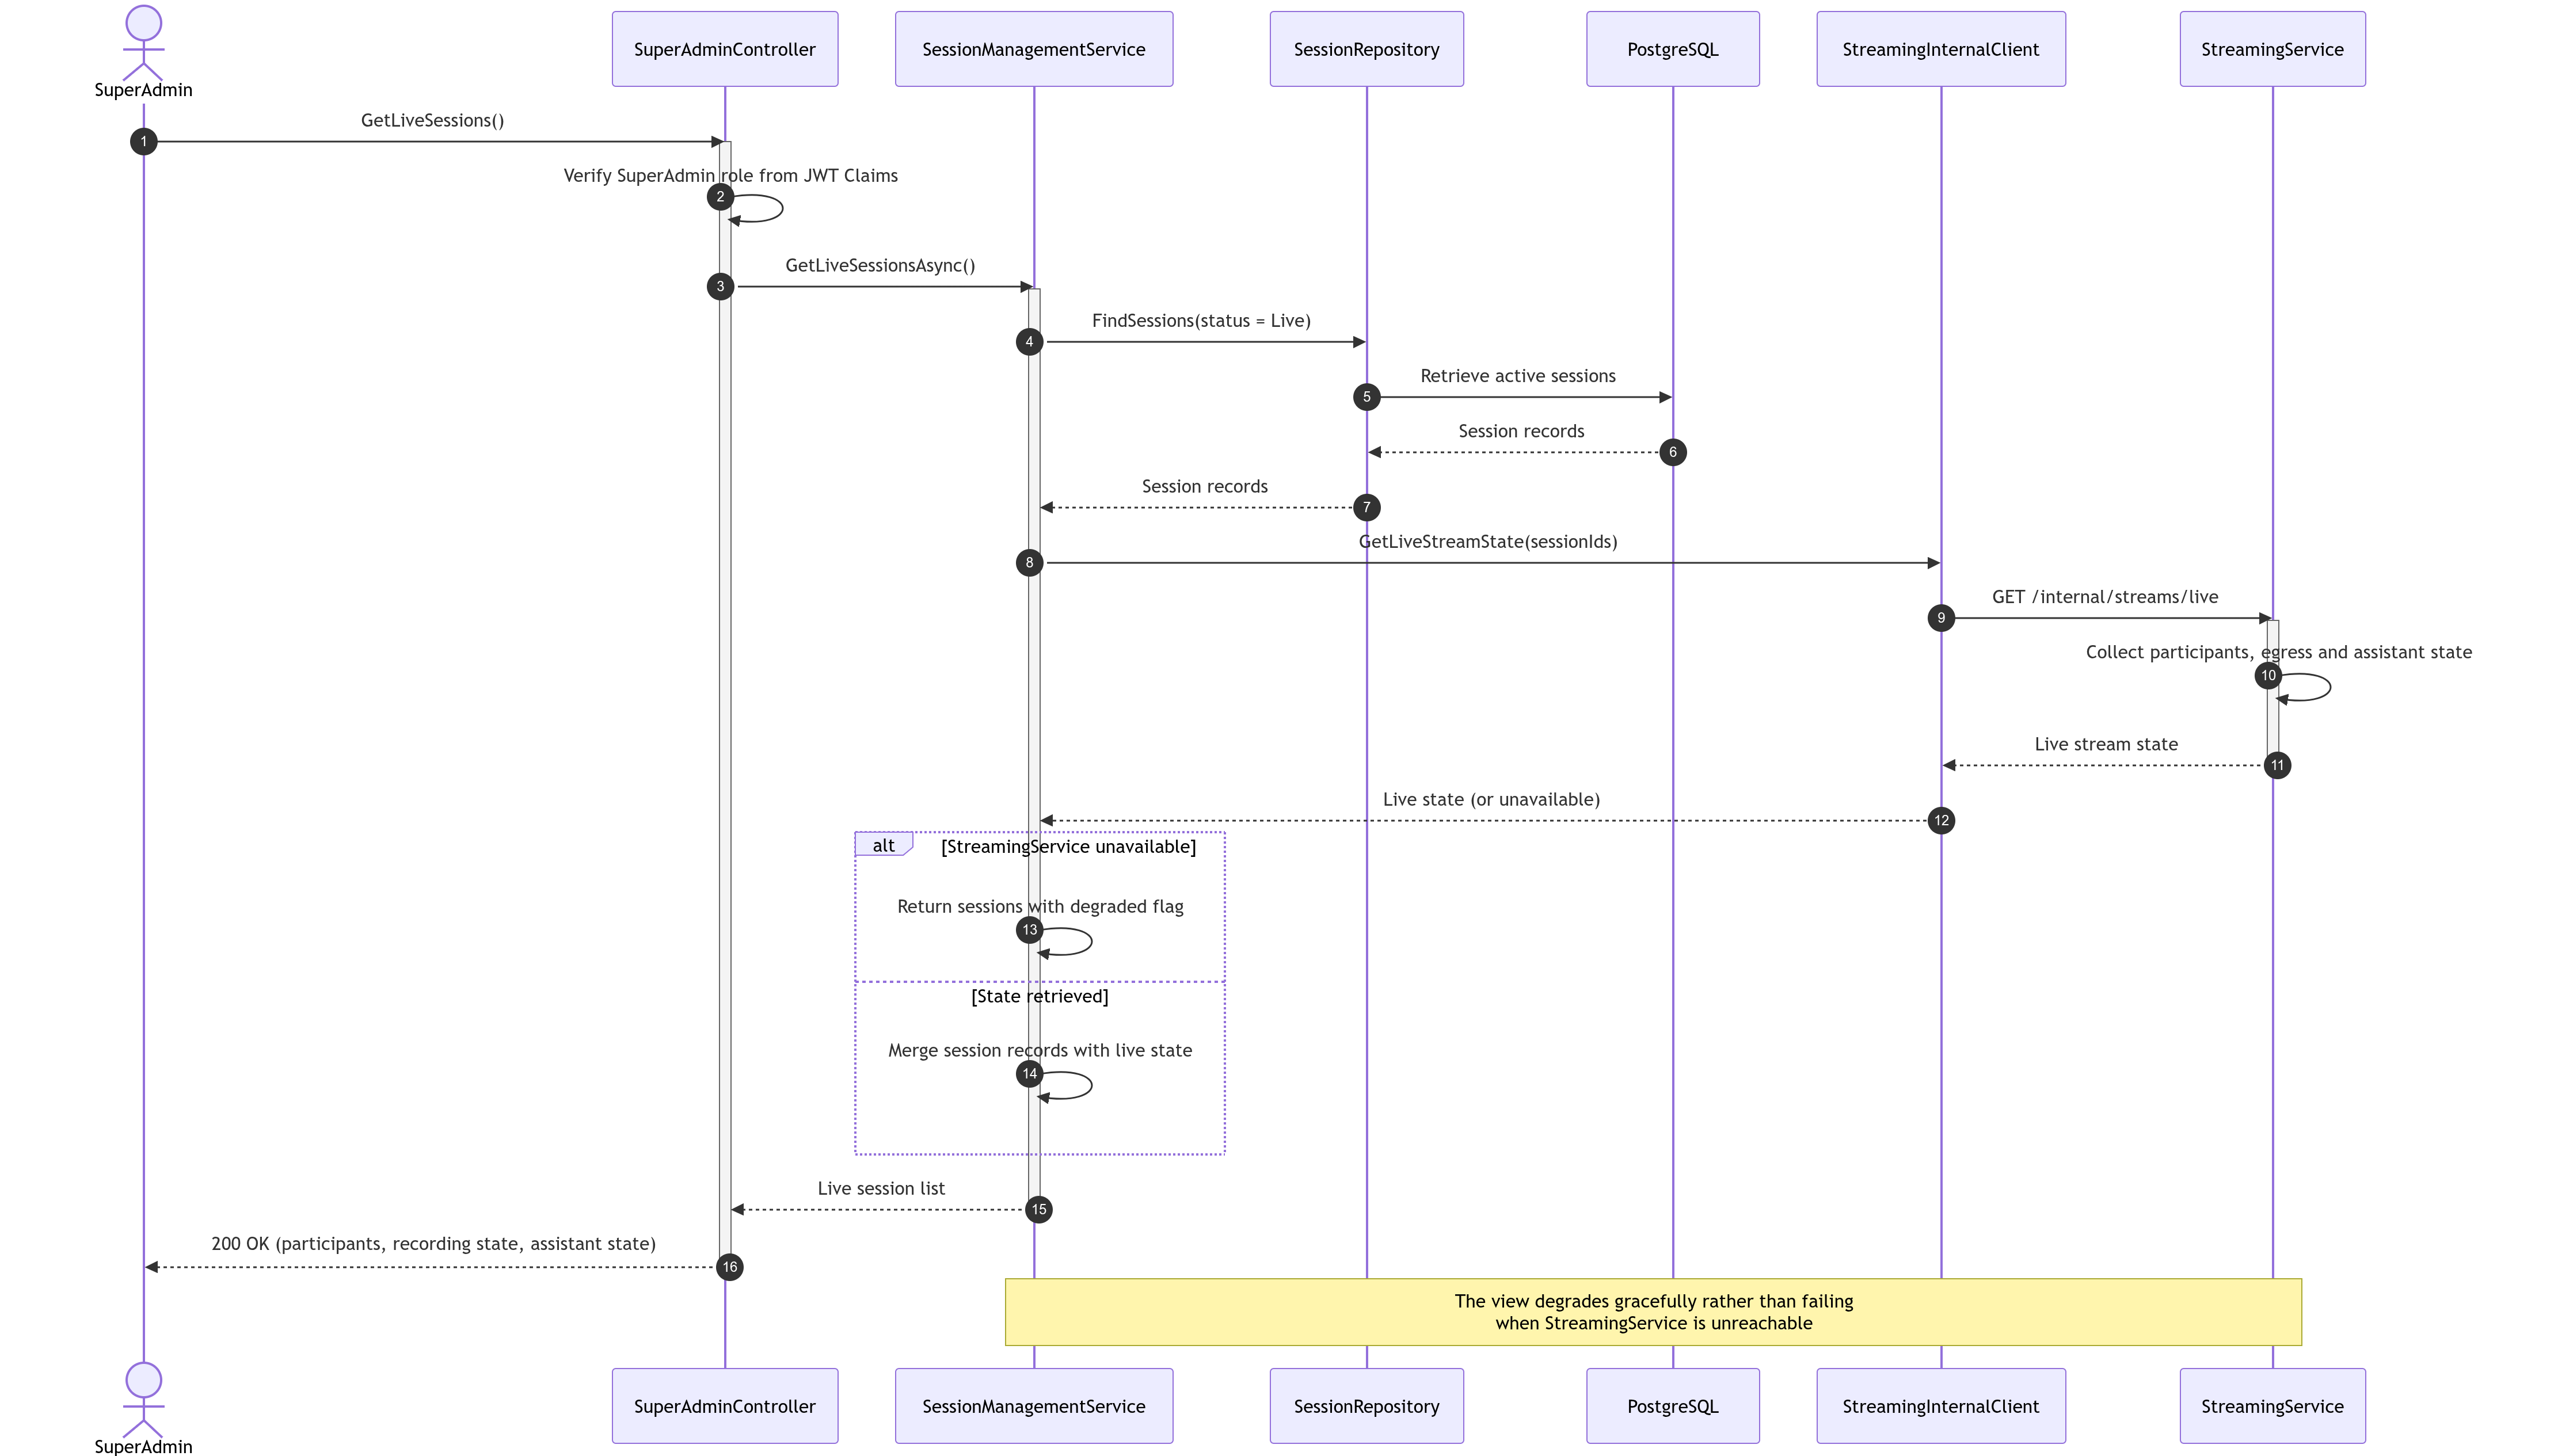
\includegraphics[width=\textwidth,height=0.8\textheight,keepaspectratio]{figures/image26.png}
  \caption{مخطط تسلسل النظام لحالة «عرض الجلسات الحية النشطة»: يوضّح الرسائل المتبادلة بين الفاعل والنظام بوصفه صندوقًا أسود، أي دون إظهار الخدمات الداخلية التي تنفّذها.}
  \label{fig:image26}
\end{figure}

\subsubsection{مخطط تسلسل النظام لحالة الإنهاء القسري لجلسة حية}

\begin{figure}[htbp]
  \centering
  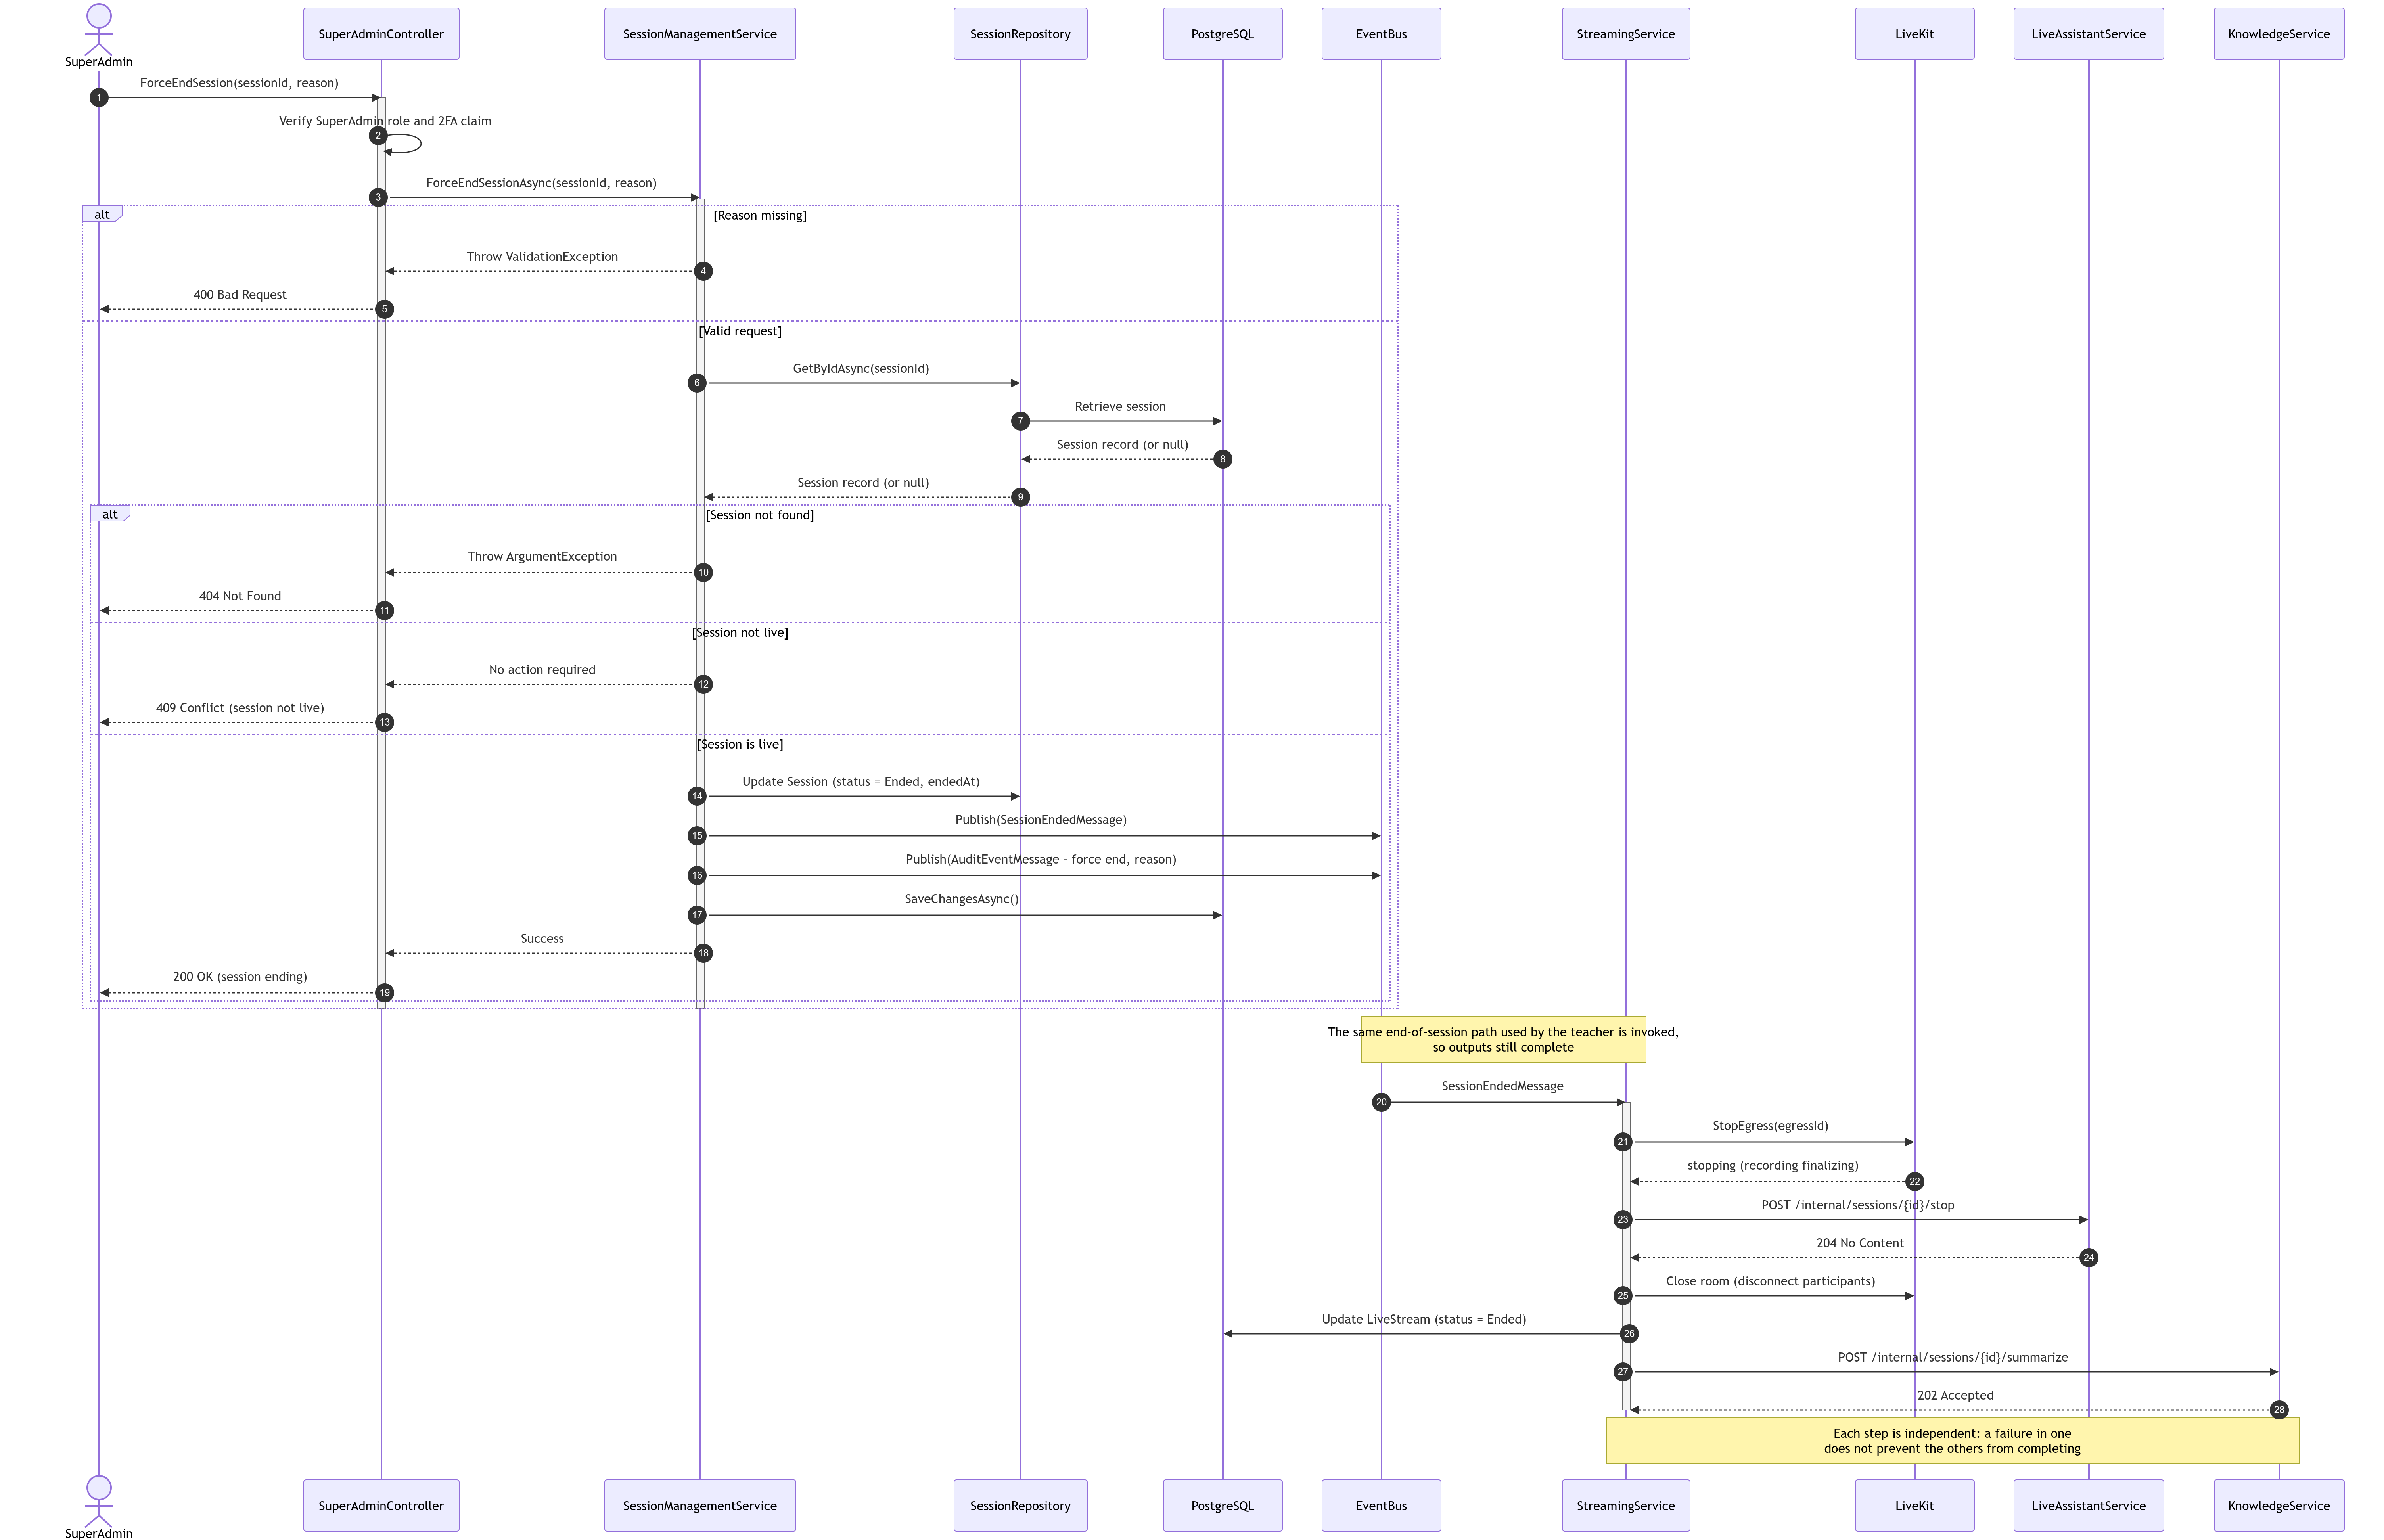
\includegraphics[width=\textwidth,height=0.8\textheight,keepaspectratio]{figures/image27.png}
  \caption{مخطط تسلسل النظام لحالة «الإنهاء القسري لجلسة حية»: يوضّح الرسائل المتبادلة بين الفاعل والنظام بوصفه صندوقًا أسود، أي دون إظهار الخدمات الداخلية التي تنفّذها.}
  \label{fig:image27}
\end{figure}

\subsection{مخطط تسلسل النظام لحالات استخدام المعلم}

\subsubsection{مخطط تسلسل النظام لحالة بدء المعلم لجلسة تعلم مباشرة}

\begin{figure}[htbp]
  \centering
  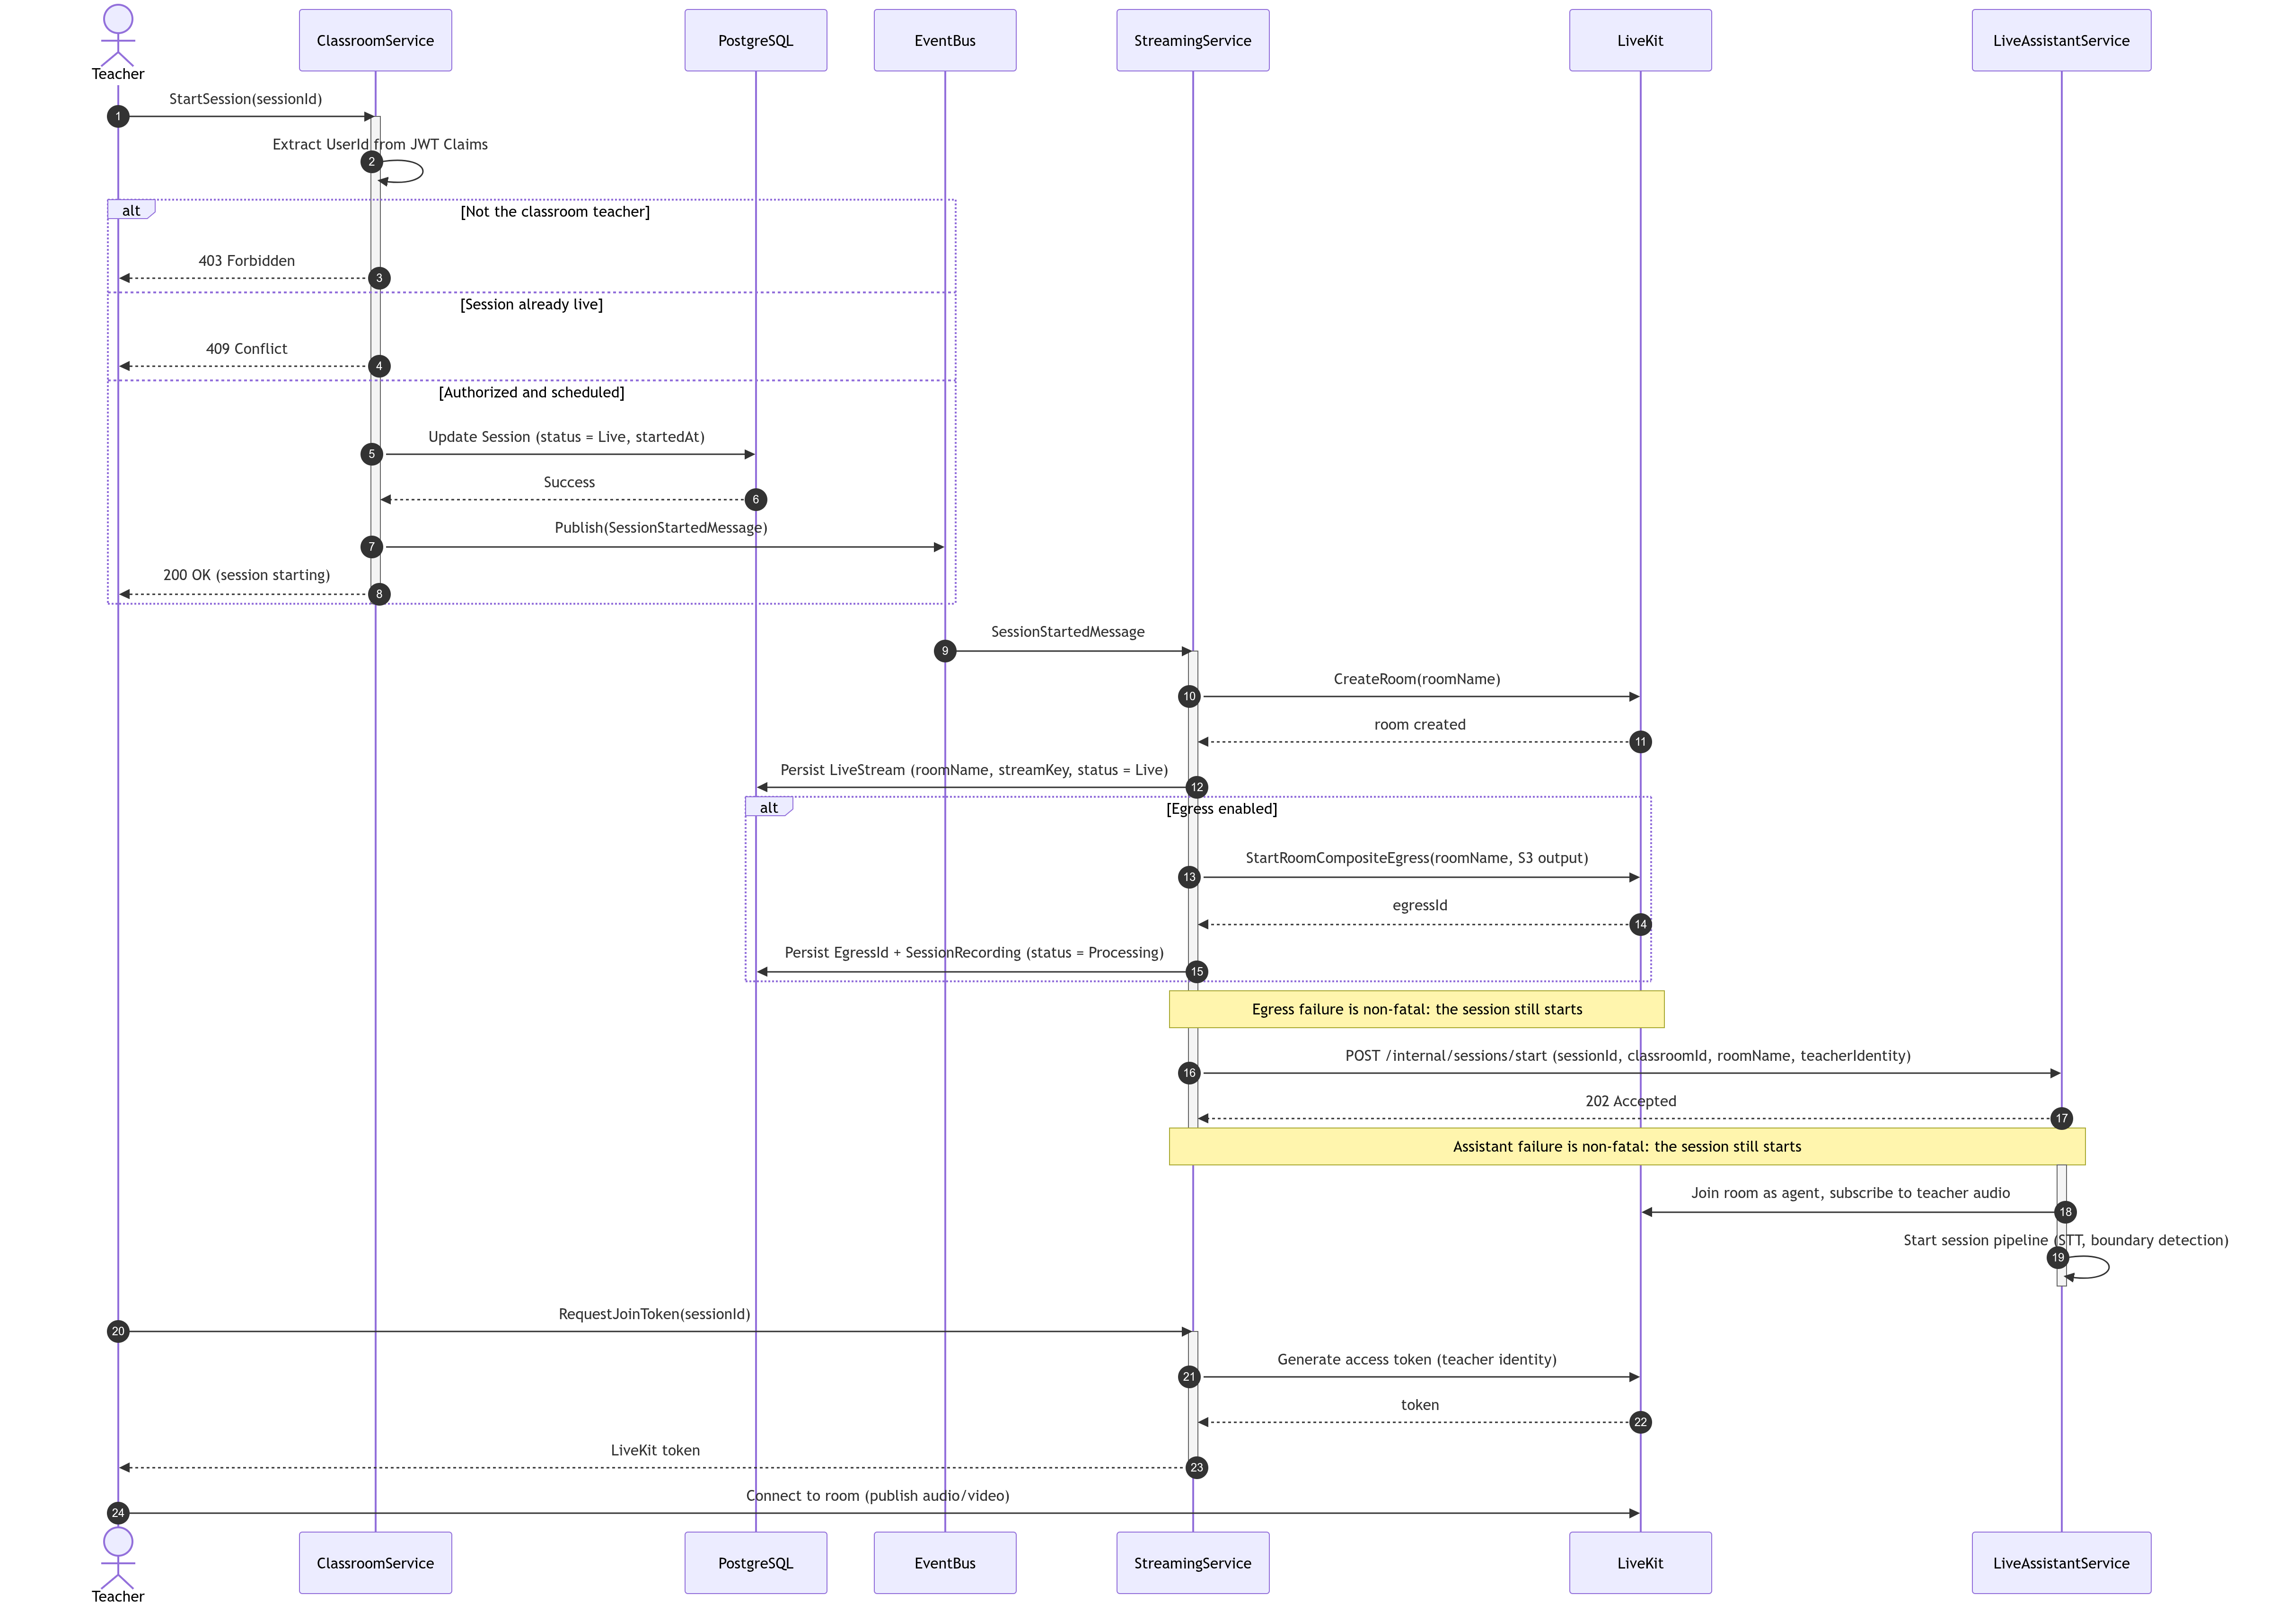
\includegraphics[width=\textwidth,height=0.8\textheight,keepaspectratio]{figures/image30.png}
  \caption{مخطط تسلسل النظام لحالة «بدء المعلم لجلسة تعلم مباشرة»: يوضّح الرسائل المتبادلة بين الفاعل والنظام بوصفه صندوقًا أسود، أي دون إظهار الخدمات الداخلية التي تنفّذها.}
  \label{fig:image30}
\end{figure}

\subsubsection{مخطط تسلسل النظام لحالة إنهاء المعلم لجلسة تعلم مباشرة}

\begin{figure}[htbp]
  \centering
  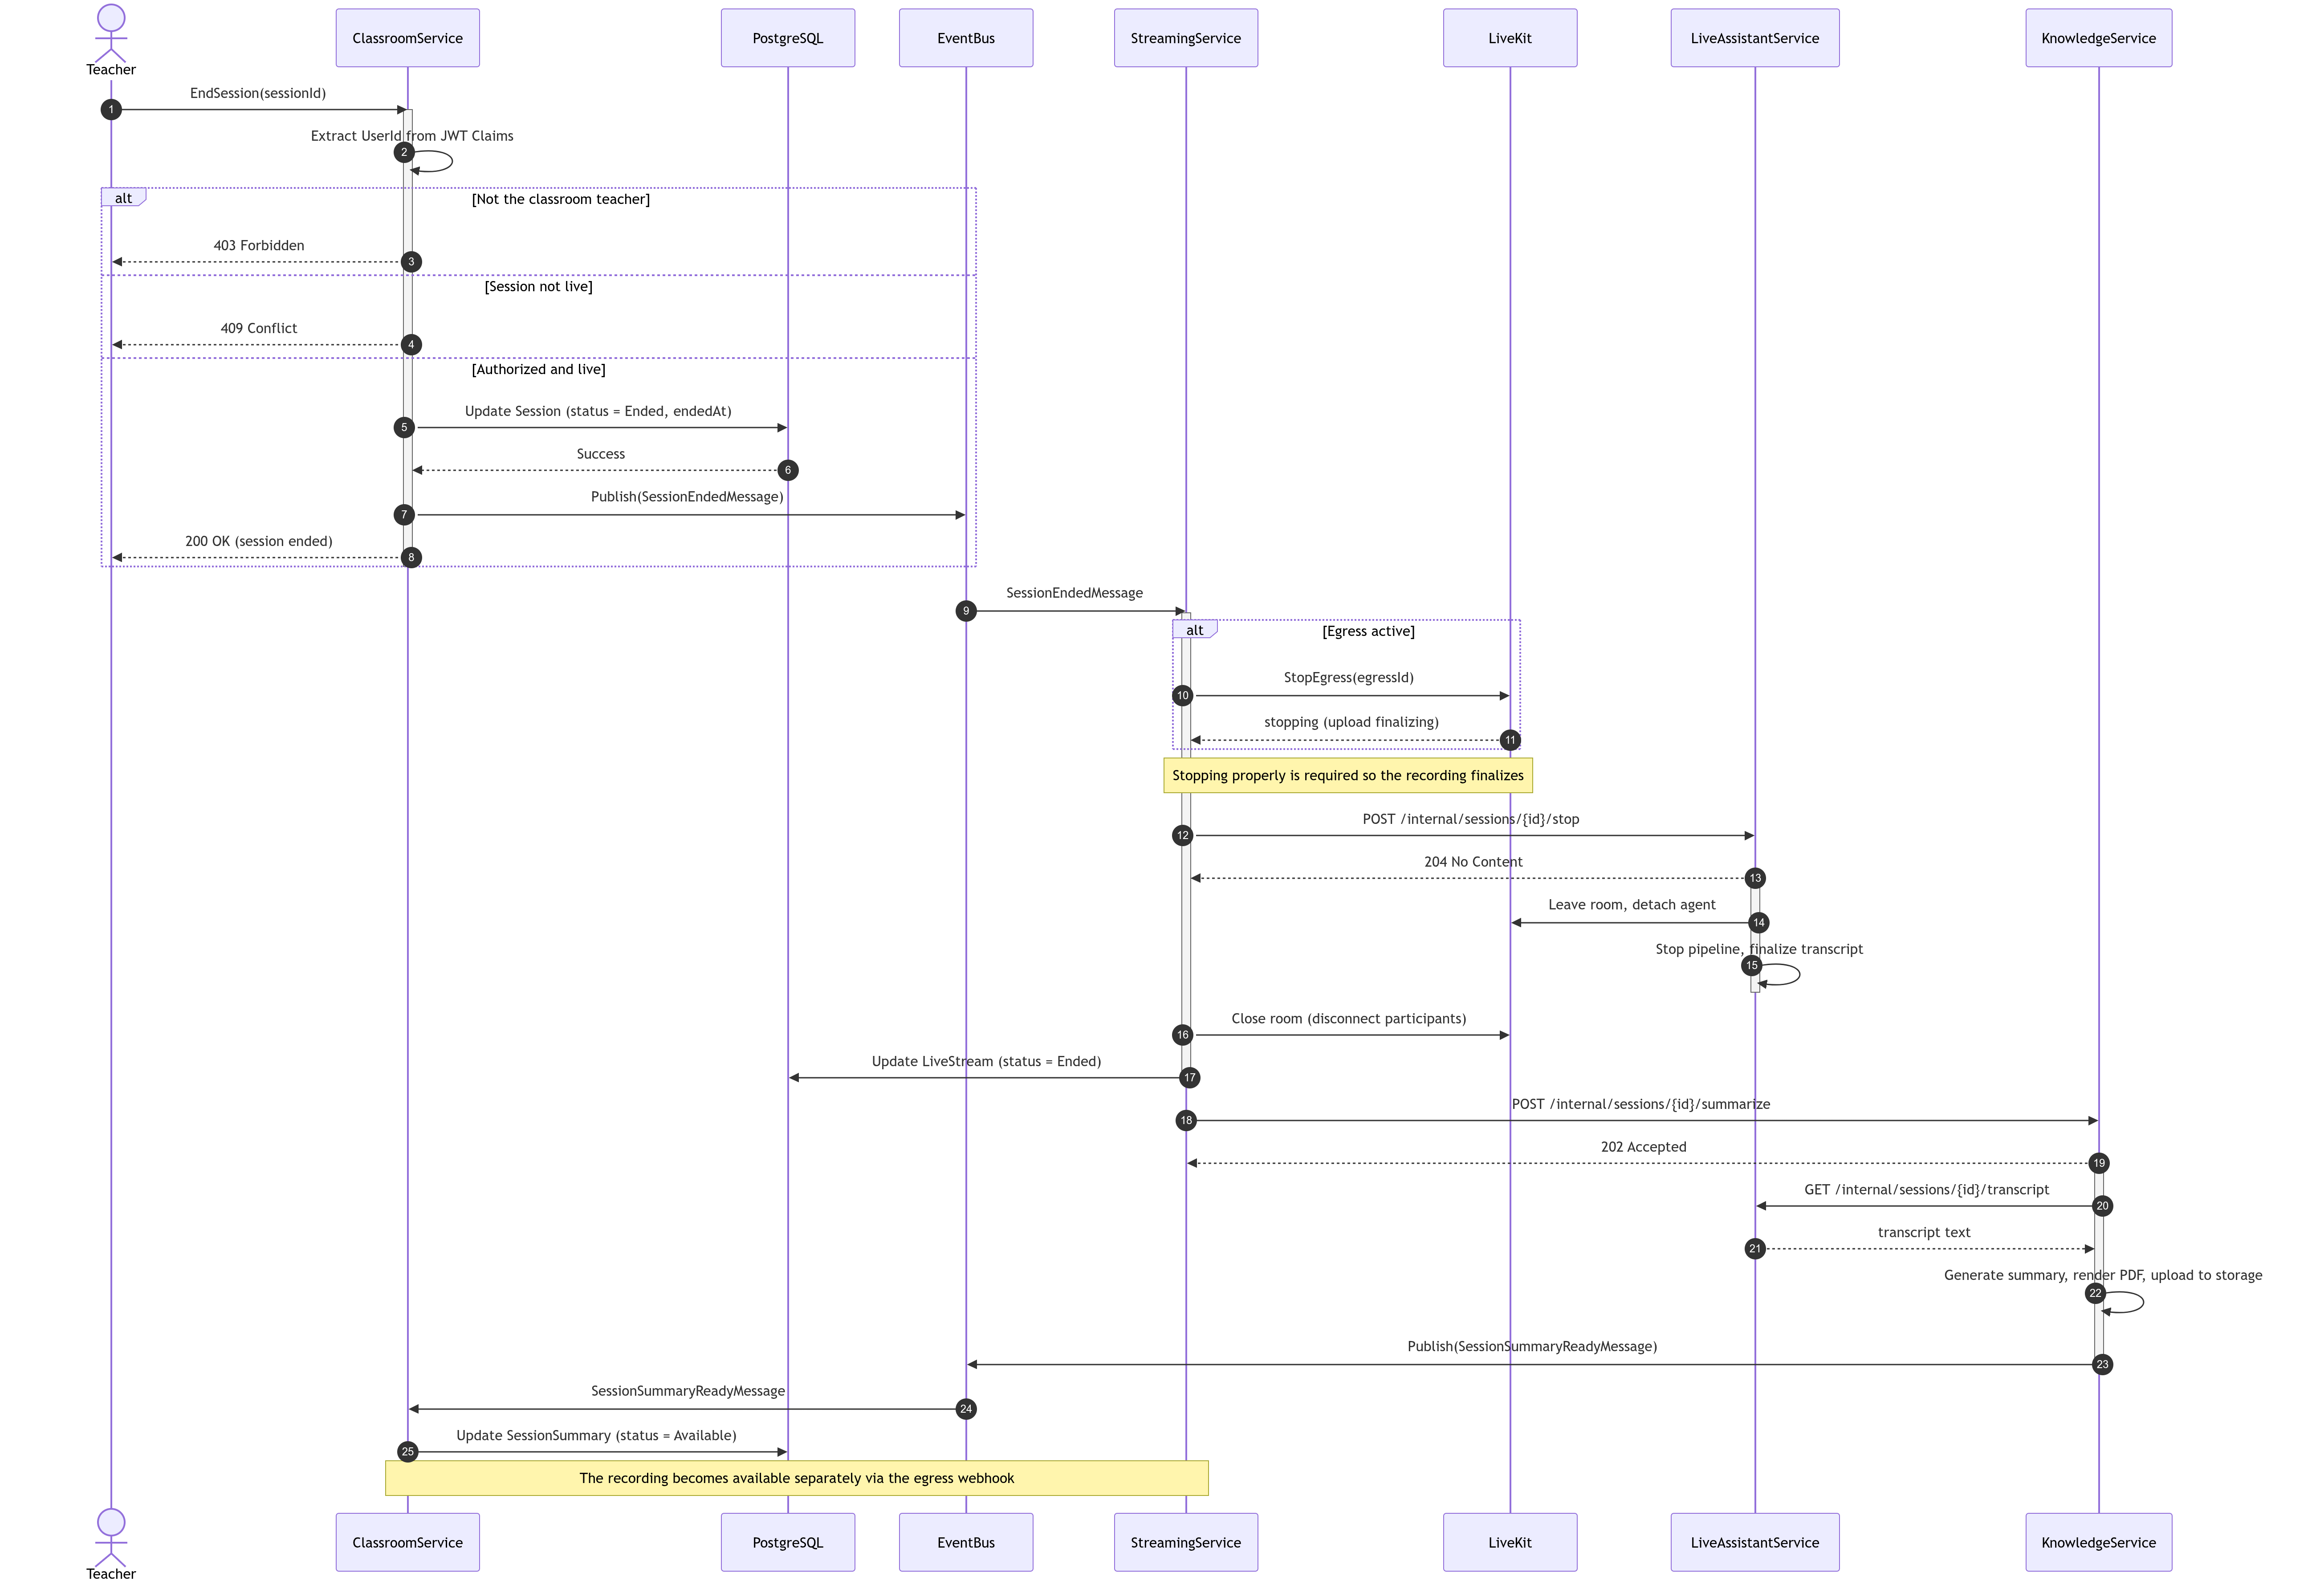
\includegraphics[width=\textwidth,height=0.8\textheight,keepaspectratio]{figures/image31.png}
  \caption{مخطط تسلسل النظام لحالة «إنهاء المعلم لجلسة تعلم مباشرة»: يوضّح الرسائل المتبادلة بين الفاعل والنظام بوصفه صندوقًا أسود، أي دون إظهار الخدمات الداخلية التي تنفّذها.}
  \label{fig:image31}
\end{figure}

\subsubsection{تدفّق إنهاء الجلسة}
\label{subsubsec:flow-session-end}

يبيّن الشكل~\ref{fig:flow-02} تدفّق إنهاء الجلسة الحيّة وما يعالجه من مشكلات السباق والذرّية والترتيب.

\begin{figure}[htbp]
  \centering
  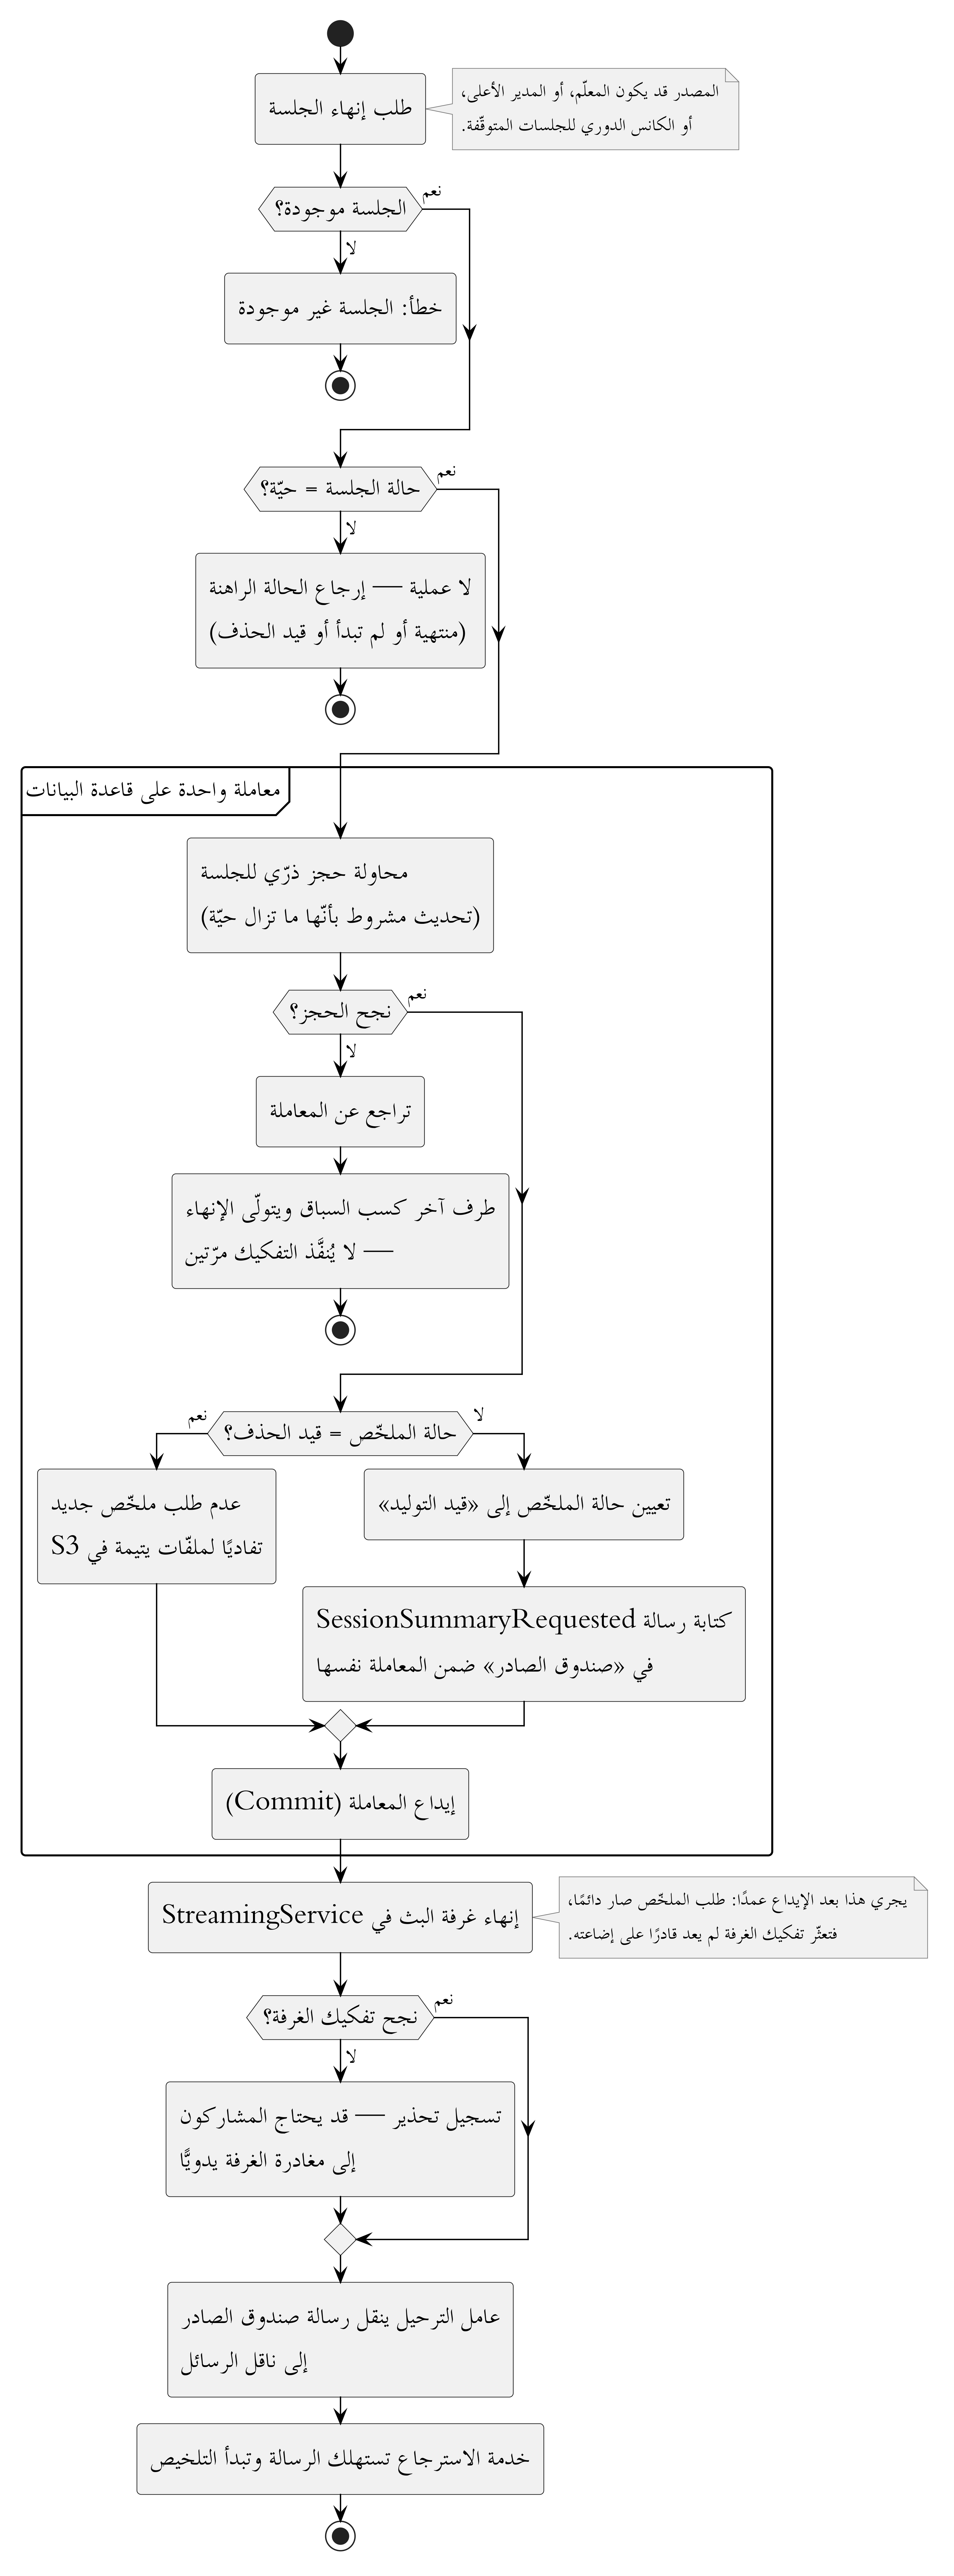
\includegraphics[width=\textwidth,height=0.8\textheight,keepaspectratio]{figures/flow-02-session-lifecycle.png}
  \caption{تدفّق إنهاء الجلسة الحيّة في خدمة الفصول الدراسية.}
  \label{fig:flow-02}
\end{figure}

\noindent تجتمع في إجرائية إنهاء الجلسة الحيّة ثلاث مشكلات صحّة منفصلة، وهي أعقد منطق في خدمة الفصول الدراسية. وقد بُيّن هذا التدفّق في الشكل~\ref{fig:flow-02}.

\begin{enumerate}
  \item \textbf{السباق} (\en{Race Condition}): يمكن أن تُنهى الجلسة من المعلّم أو المدير الأعلى أو الكانس الدوري في اللحظة نفسها. واستُعمل تحديثٌ ذرّيٌّ مشروط يُسنِد الفصل في التزامن إلى قاعدة البيانات: يتولّى التفكيك من ينجح في الحجز، ويتوقّف من يفشل فيه، فلا يُنفَّذ التفكيك مرّتين.
  \item \textbf{الذرّية} (\en{Atomicity}): يجب أن يُحفَظ تغيّرُ حالة الجلسة وتسجيلُ استحقاق الملخّص معًا أو لا يُحفَظ أيٌّ منهما. ولذلك تُكتَب رسالة طلب الملخّص في جدول صندوق الصادر ضمن المعاملة نفسها، ثمّ يُرحّلها عاملٌ مستقلّ إلى الناقل لاحقًا، بدلًا من نشرها مباشرةً.
  \item \textbf{الترتيب} (\en{Ordering}): يجري تفكيك غرفة البث بعد إيداع المعاملة. ويُبنى الملخّص من النصّ الذي يُفرِغه المساعد المباشر عند التفكيك، وقد صار طلب الملخّص محفوظًا في قاعدة البيانات قبل ذلك. ولا يؤدّي بطء تفكيك الغرفة أو تعثّره عندئذٍ إلى فقد الملخّص.
\end{enumerate}

\subsubsection{مخطط تسلسل النظام لحالة انضمام الطالب إلى جلسة تعلم مباشرة}

\begin{figure}[htbp]
  \centering
  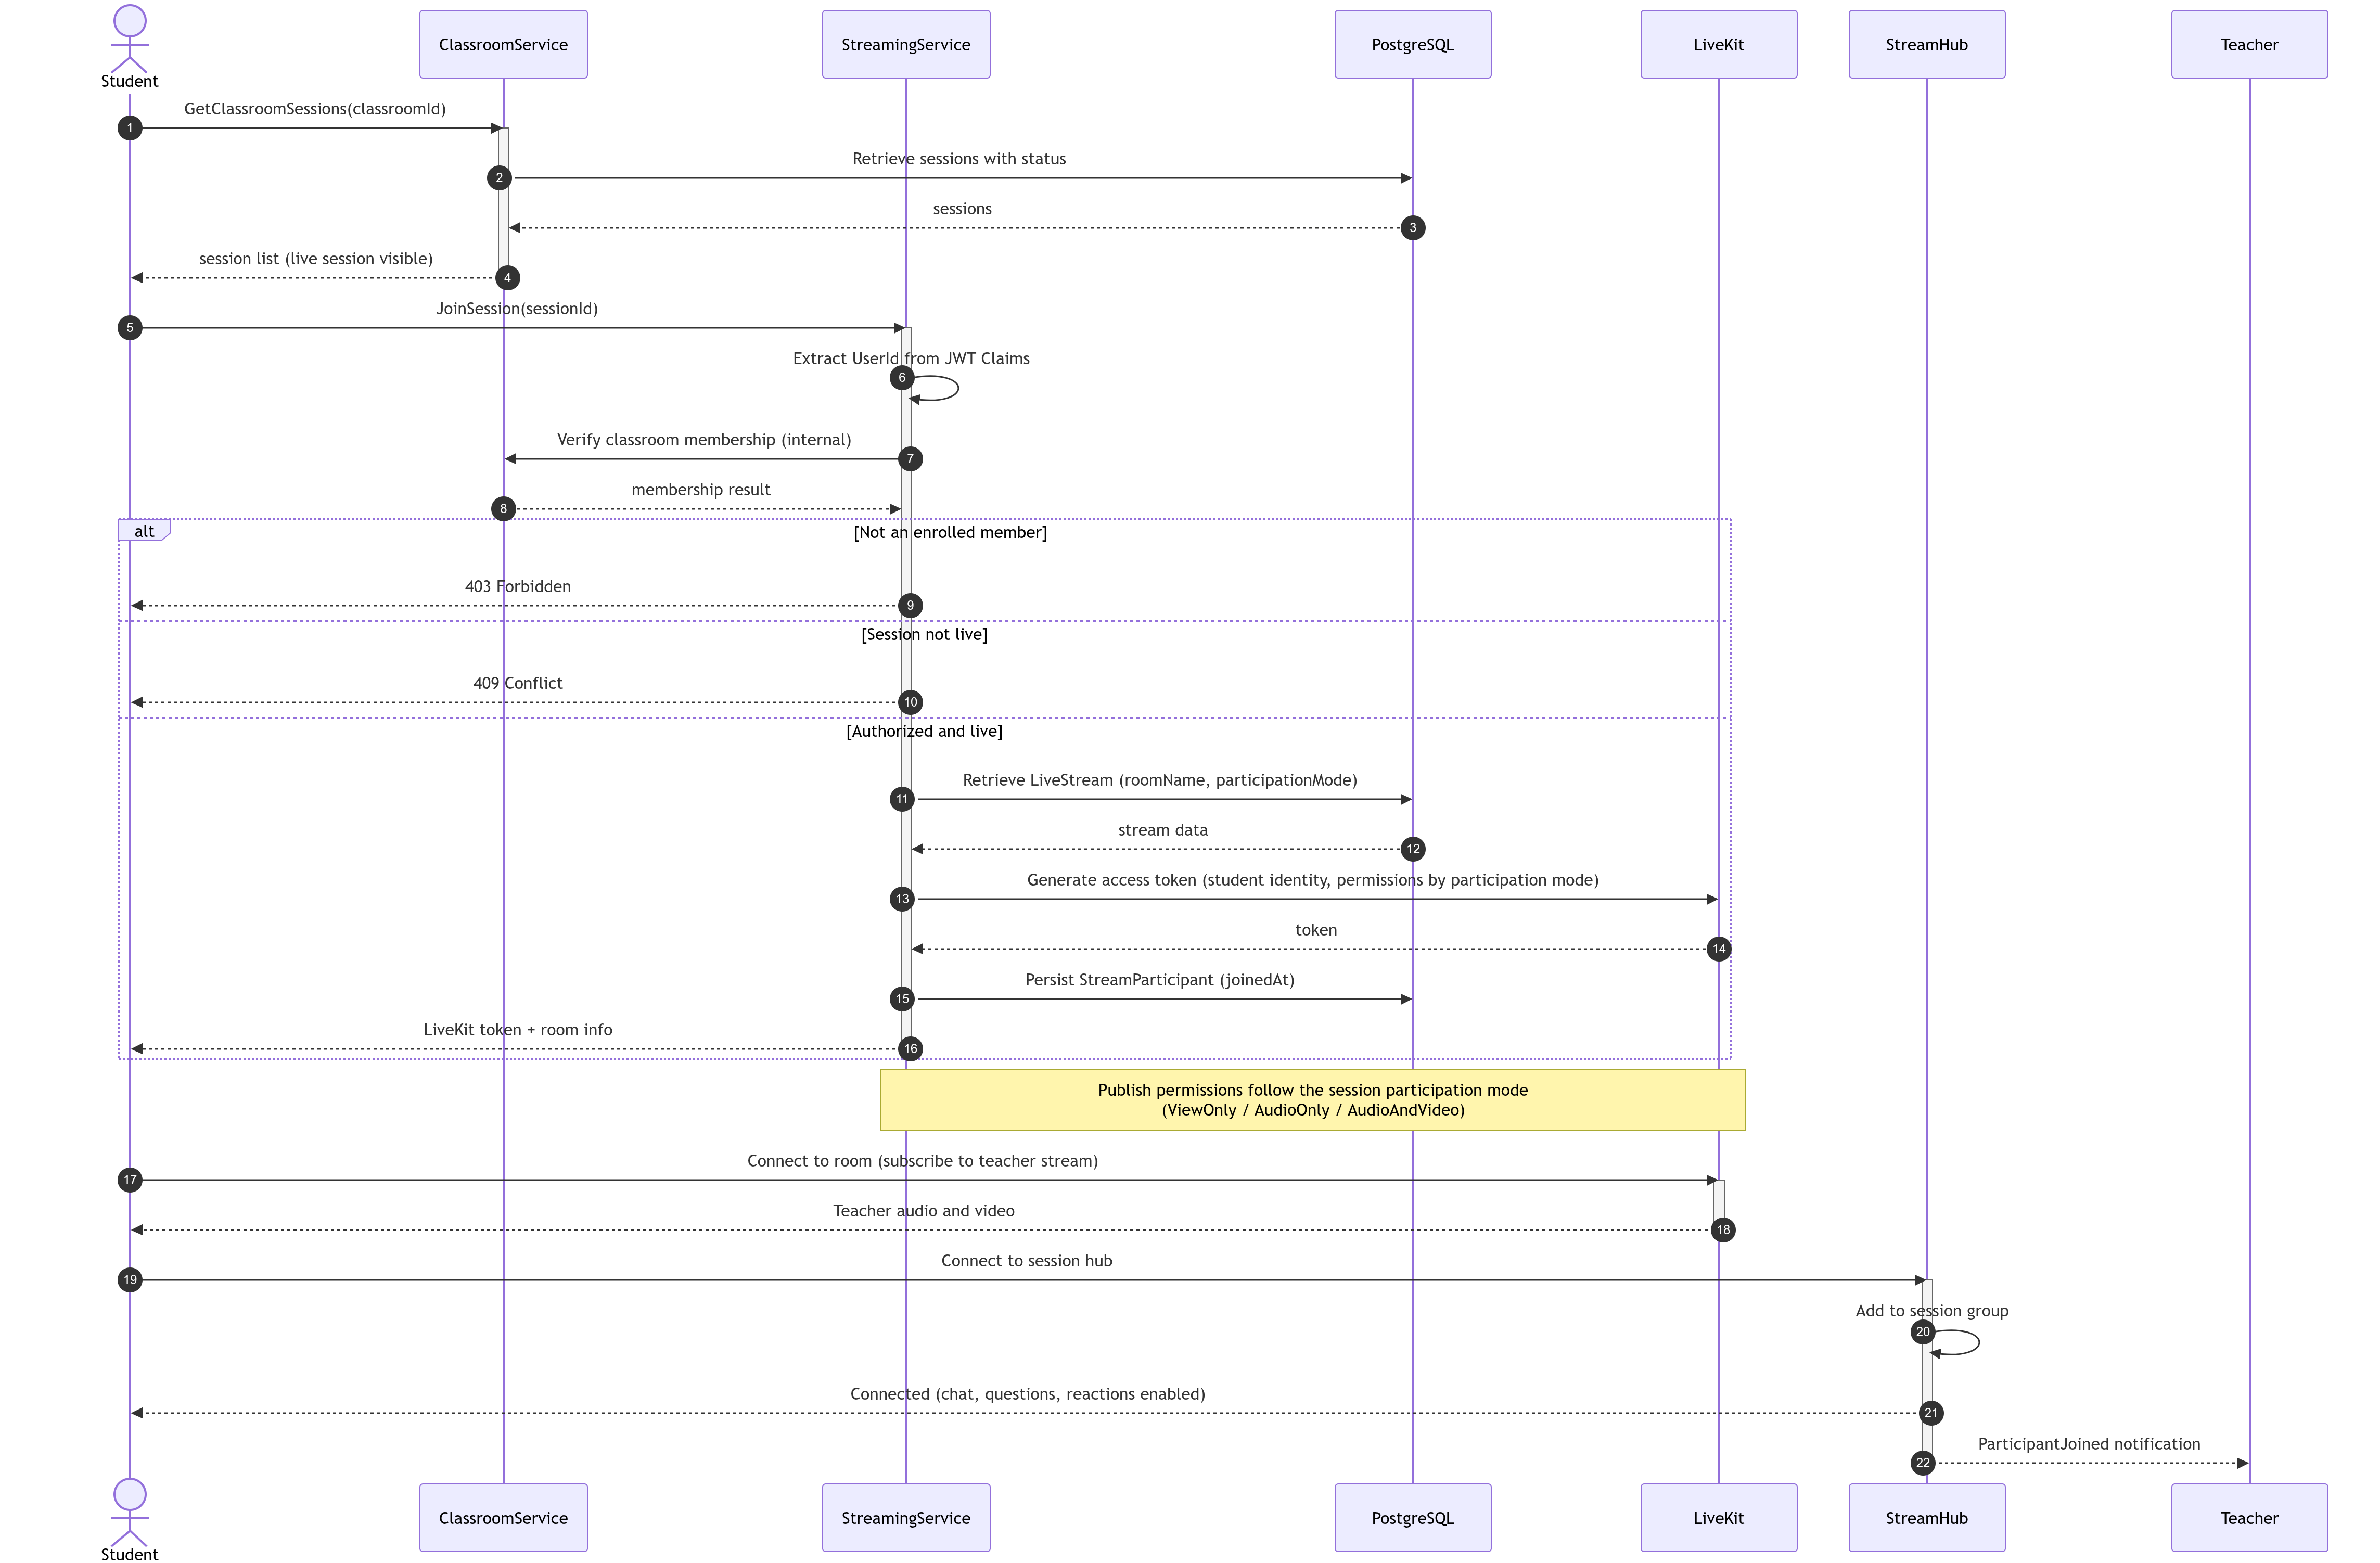
\includegraphics[width=\textwidth,height=0.8\textheight,keepaspectratio]{figures/image32.png}
  \caption{مخطط تسلسل النظام لحالة «انضمام الطالب إلى جلسة تعلم مباشرة»: يوضّح الرسائل المتبادلة بين الفاعل والنظام بوصفه صندوقًا أسود، أي دون إظهار الخدمات الداخلية التي تنفّذها.}
  \label{fig:image32}
\end{figure}

\subsubsection{مخطط تسلسل النظام لحالة التفاعل داخل جلسة التعلم المباشرة}

\begin{figure}[htbp]
  \centering
  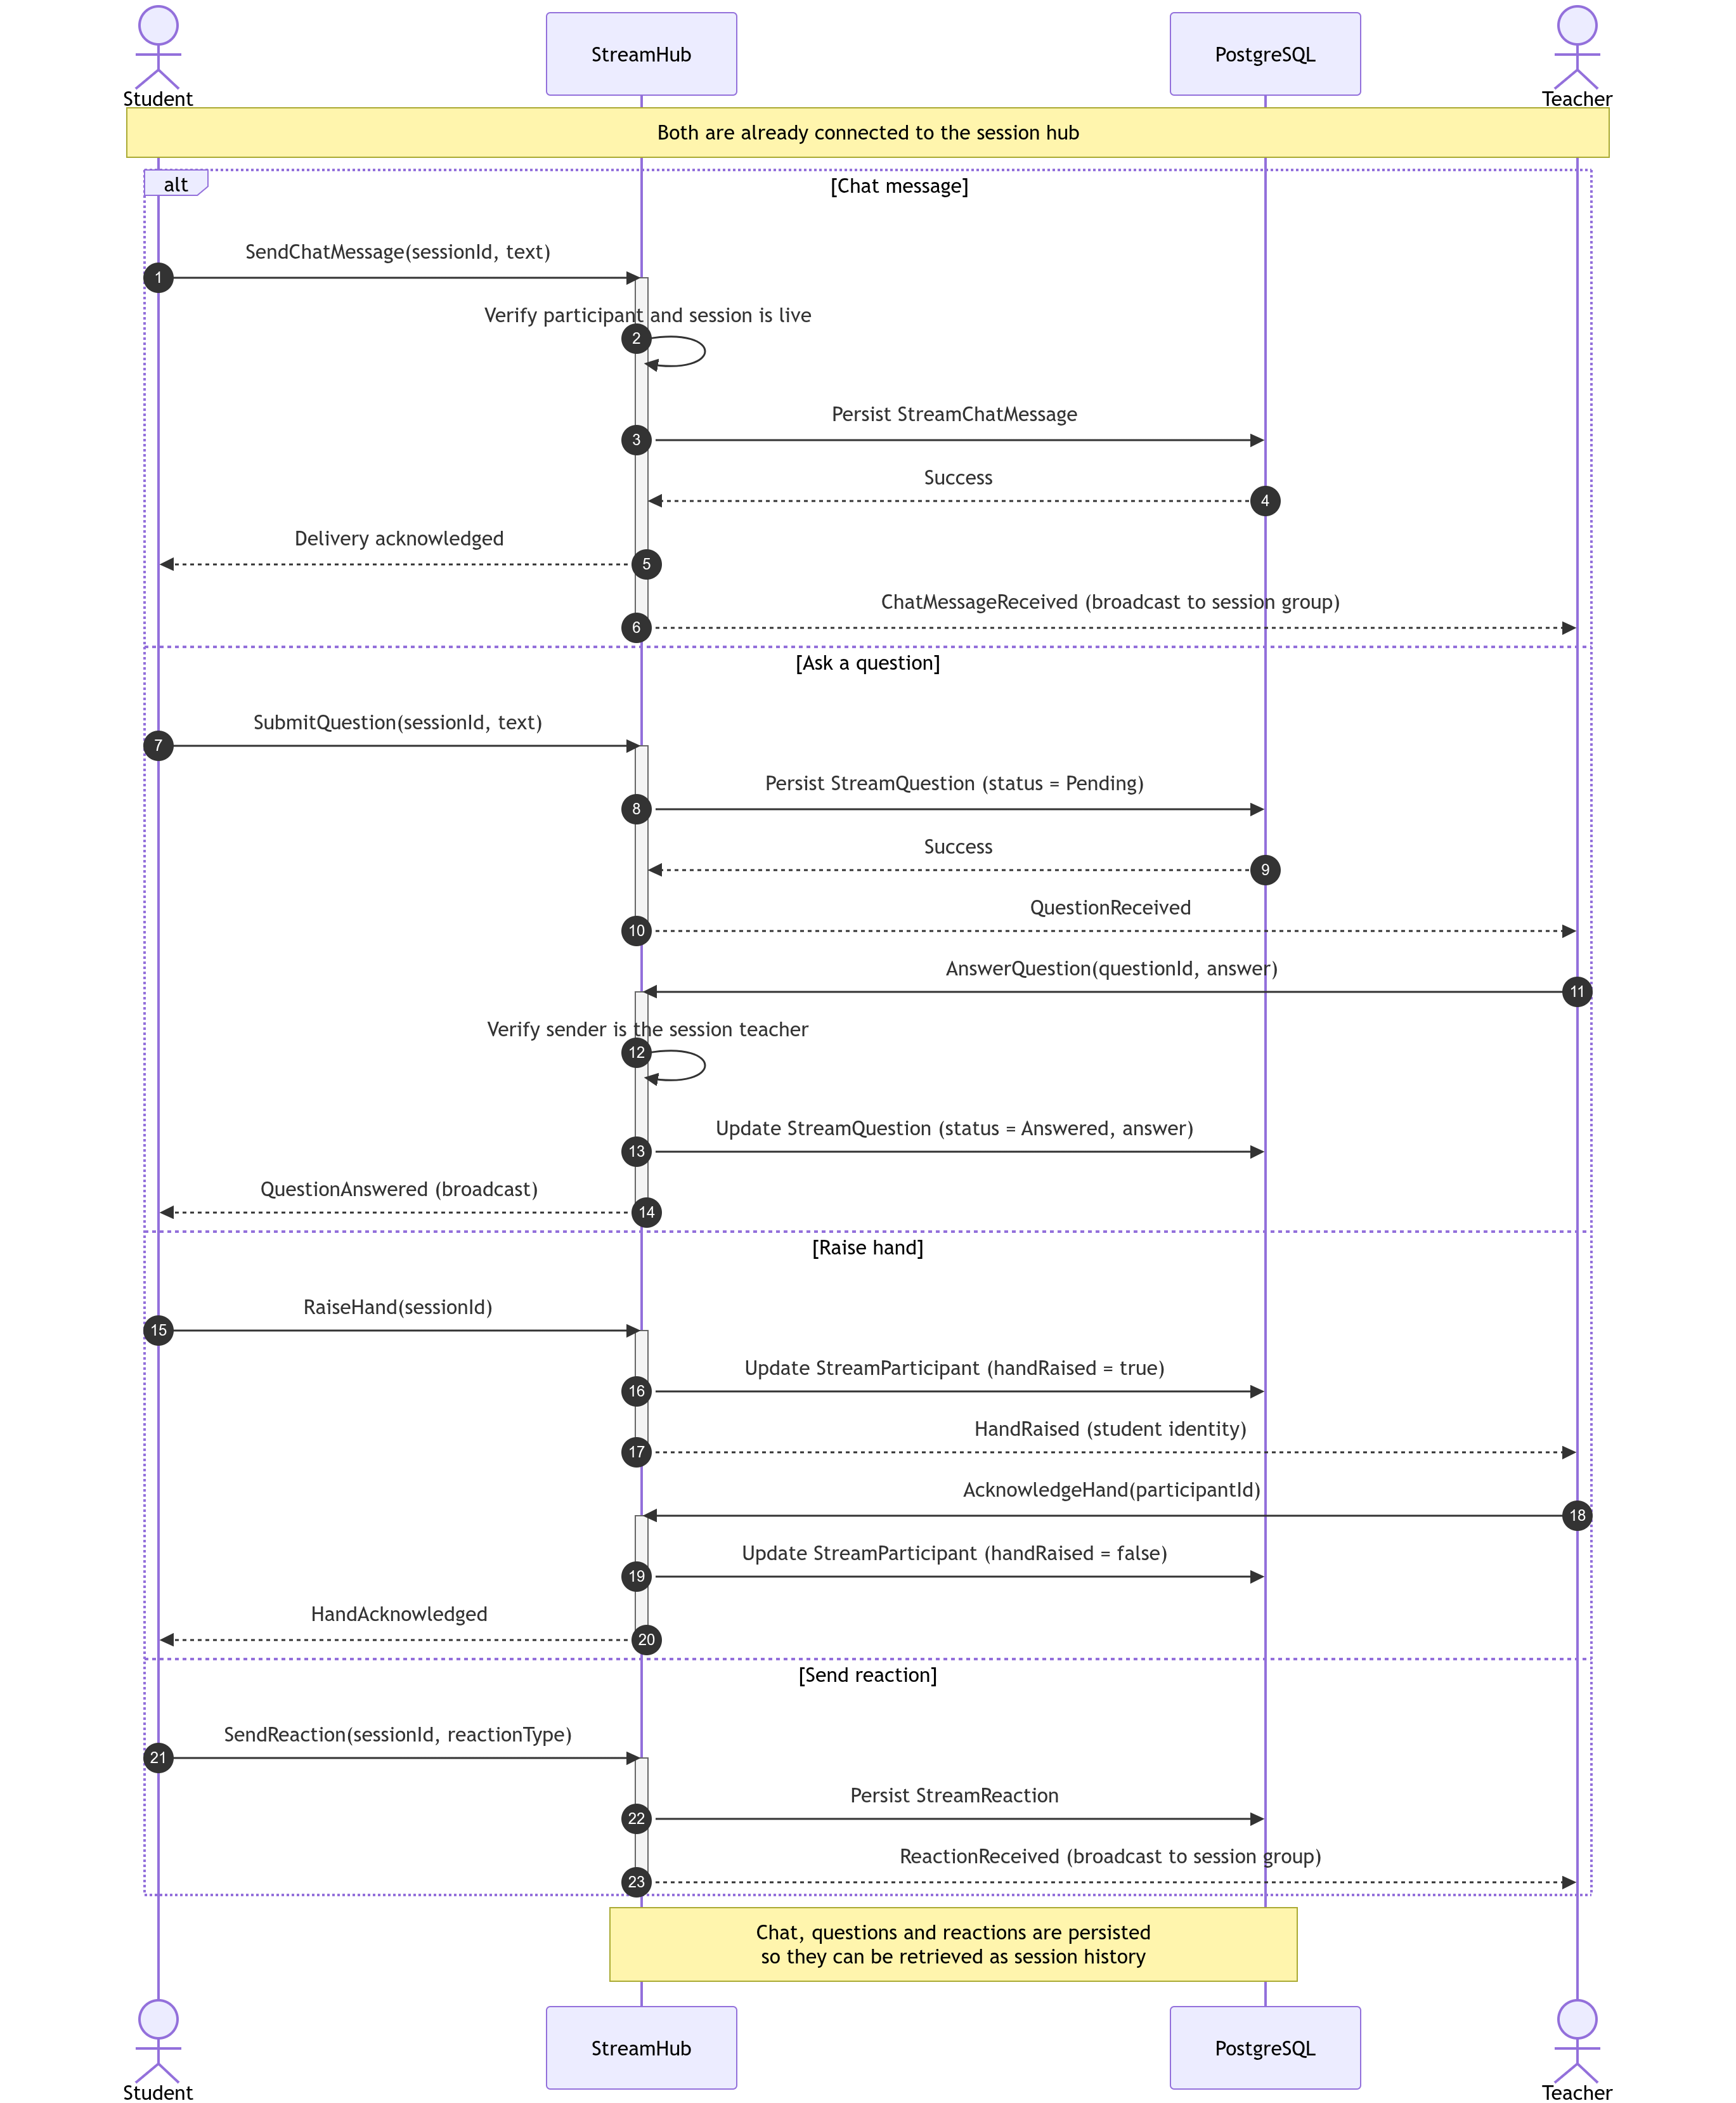
\includegraphics[width=\textwidth,height=0.8\textheight,keepaspectratio]{figures/image33.png}
  \caption{مخطط تسلسل النظام لحالة «التفاعل داخل جلسة التعلم المباشرة»: يوضّح الرسائل المتبادلة بين الفاعل والنظام بوصفه صندوقًا أسود، أي دون إظهار الخدمات الداخلية التي تنفّذها.}
  \label{fig:image33}
\end{figure}

\subsubsection{مخطط تسلسل النظام لحالة الإجابة عن سؤال الطالب اعتمادًا على مواد الفصل}

\begin{figure}[htbp]
  \centering
  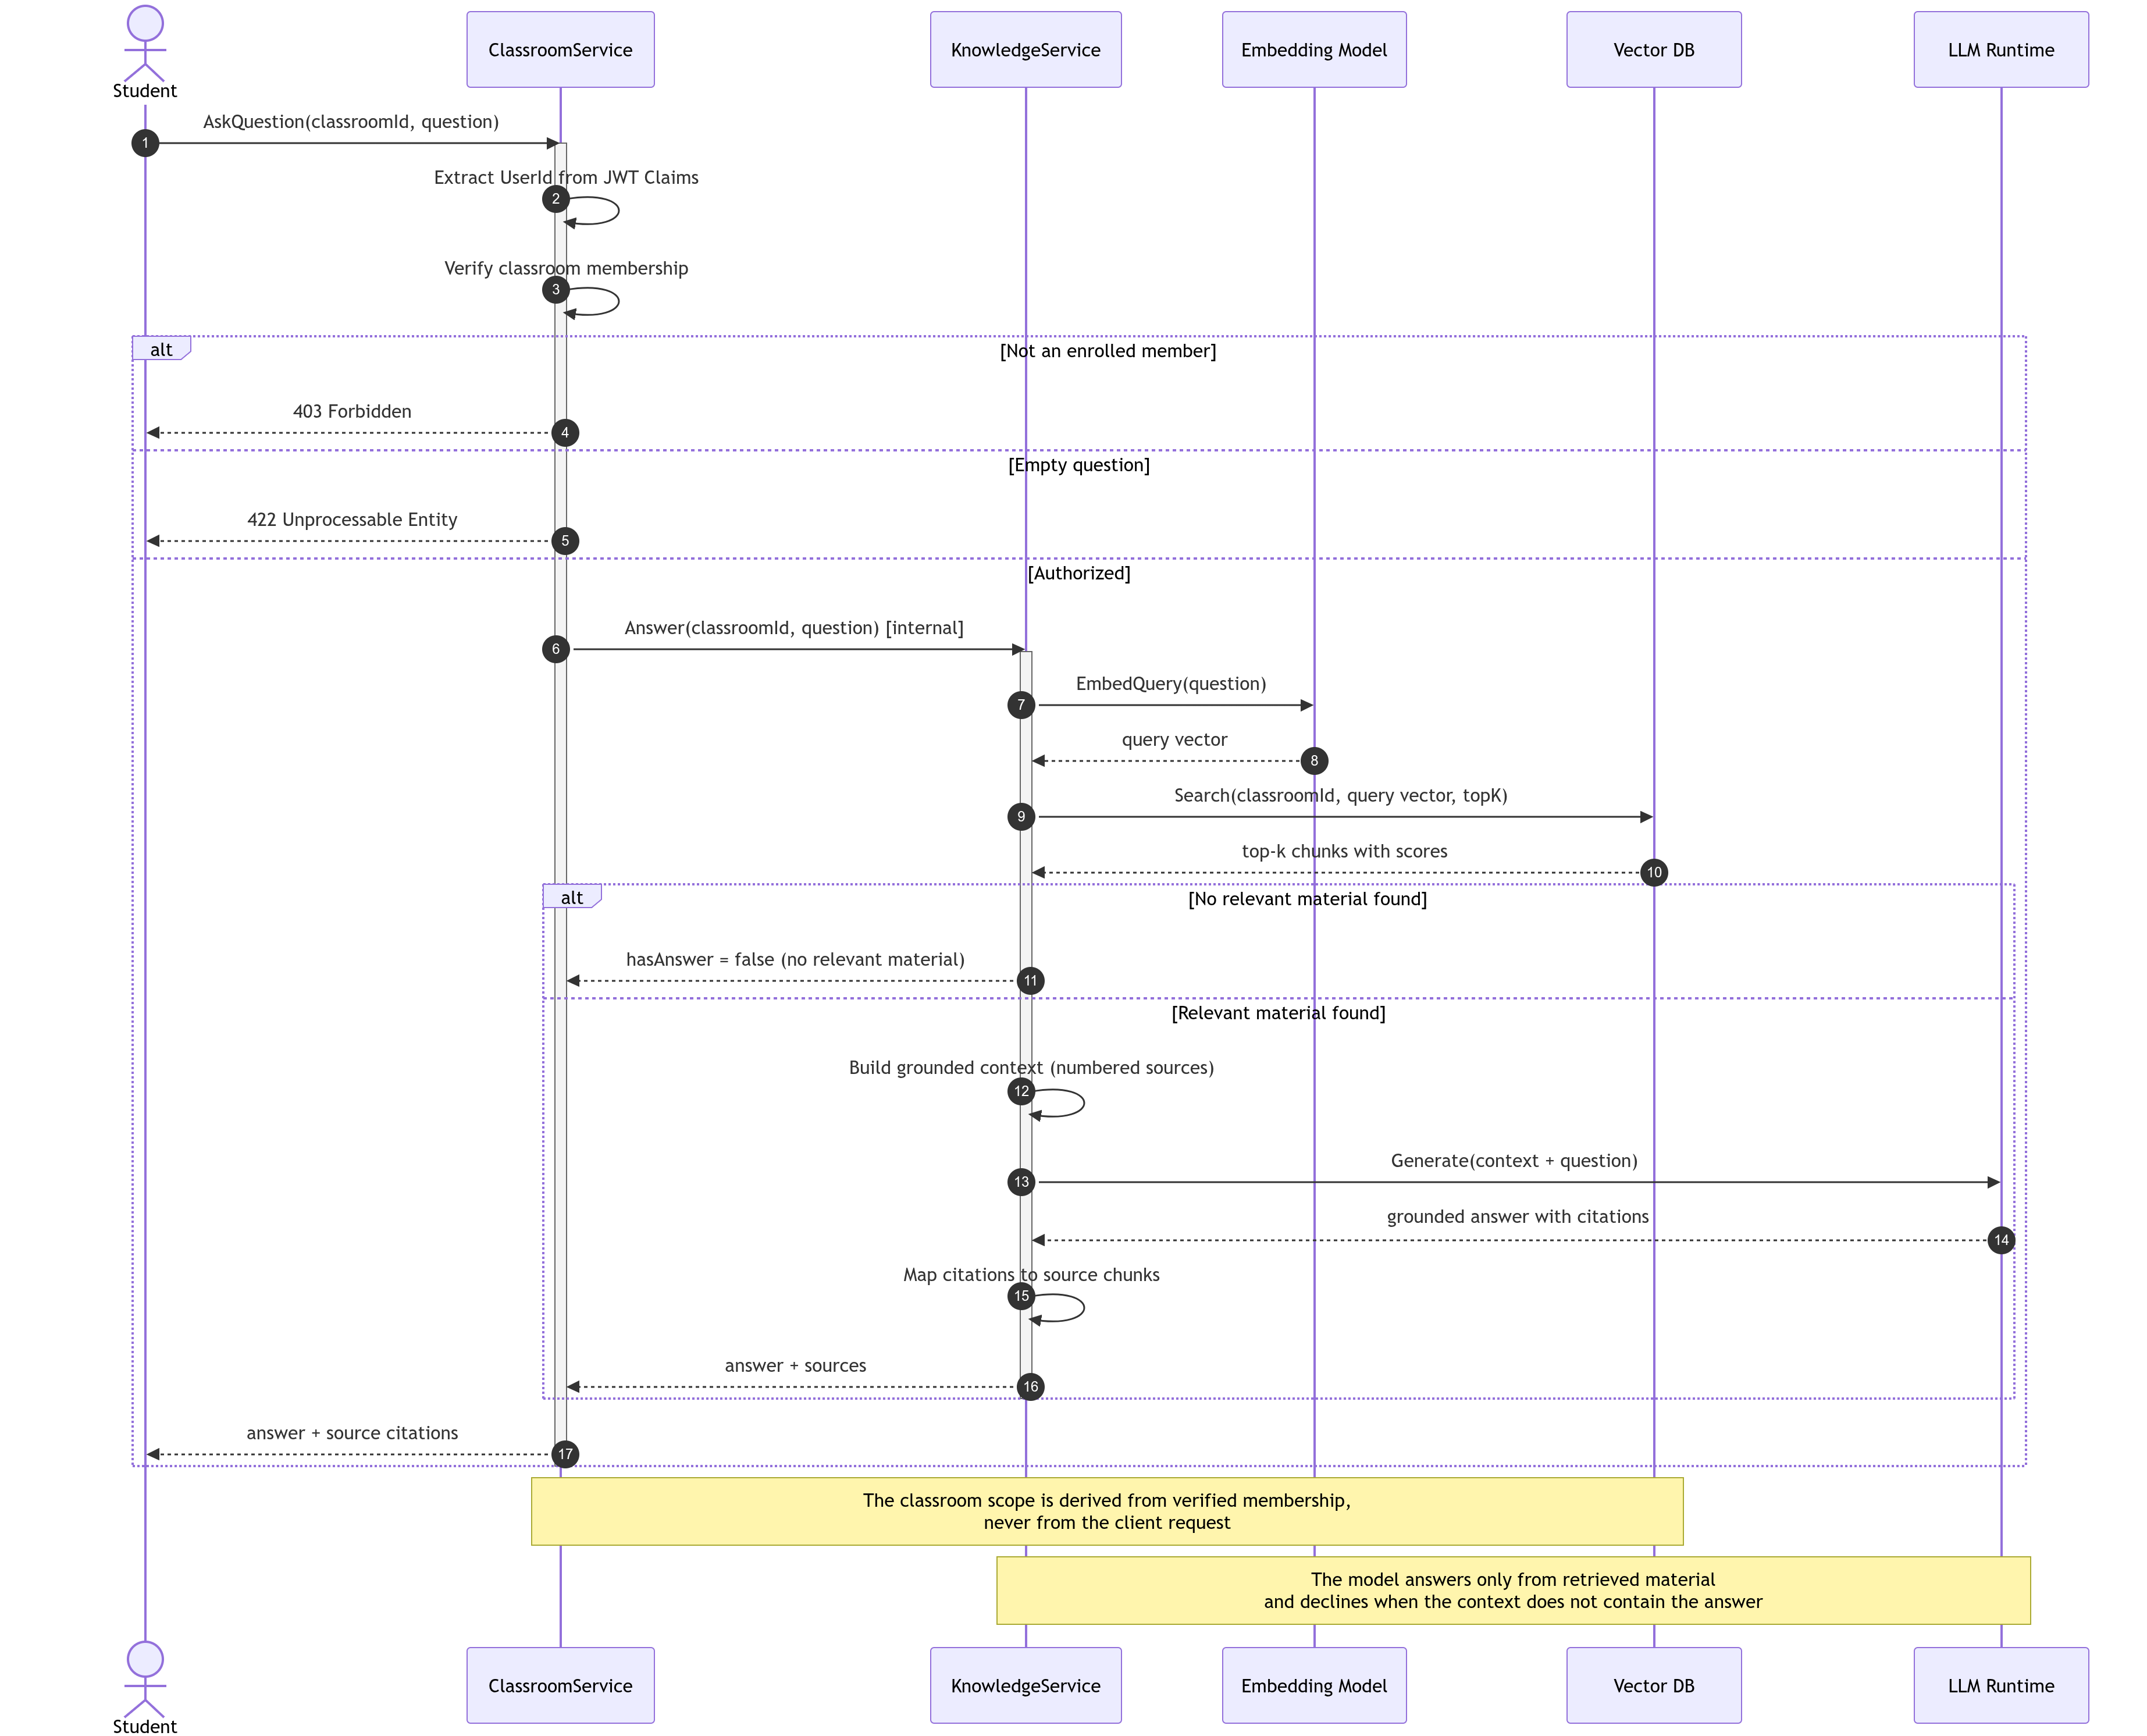
\includegraphics[width=\textwidth,height=0.8\textheight,keepaspectratio]{figures/image34.png}
  \caption{مخطط تسلسل النظام لحالة «الإجابة عن سؤال الطالب اعتمادًا على مواد الفصل»: يوضّح الرسائل المتبادلة بين الفاعل والنظام بوصفه صندوقًا أسود، أي دون إظهار الخدمات الداخلية التي تنفّذها.}
  \label{fig:image34}
\end{figure}

\subsubsection{مخطط تسلسل النظام لحالة توليد ملخّص الجلسة}

\begin{figure}[htbp]
  \centering
  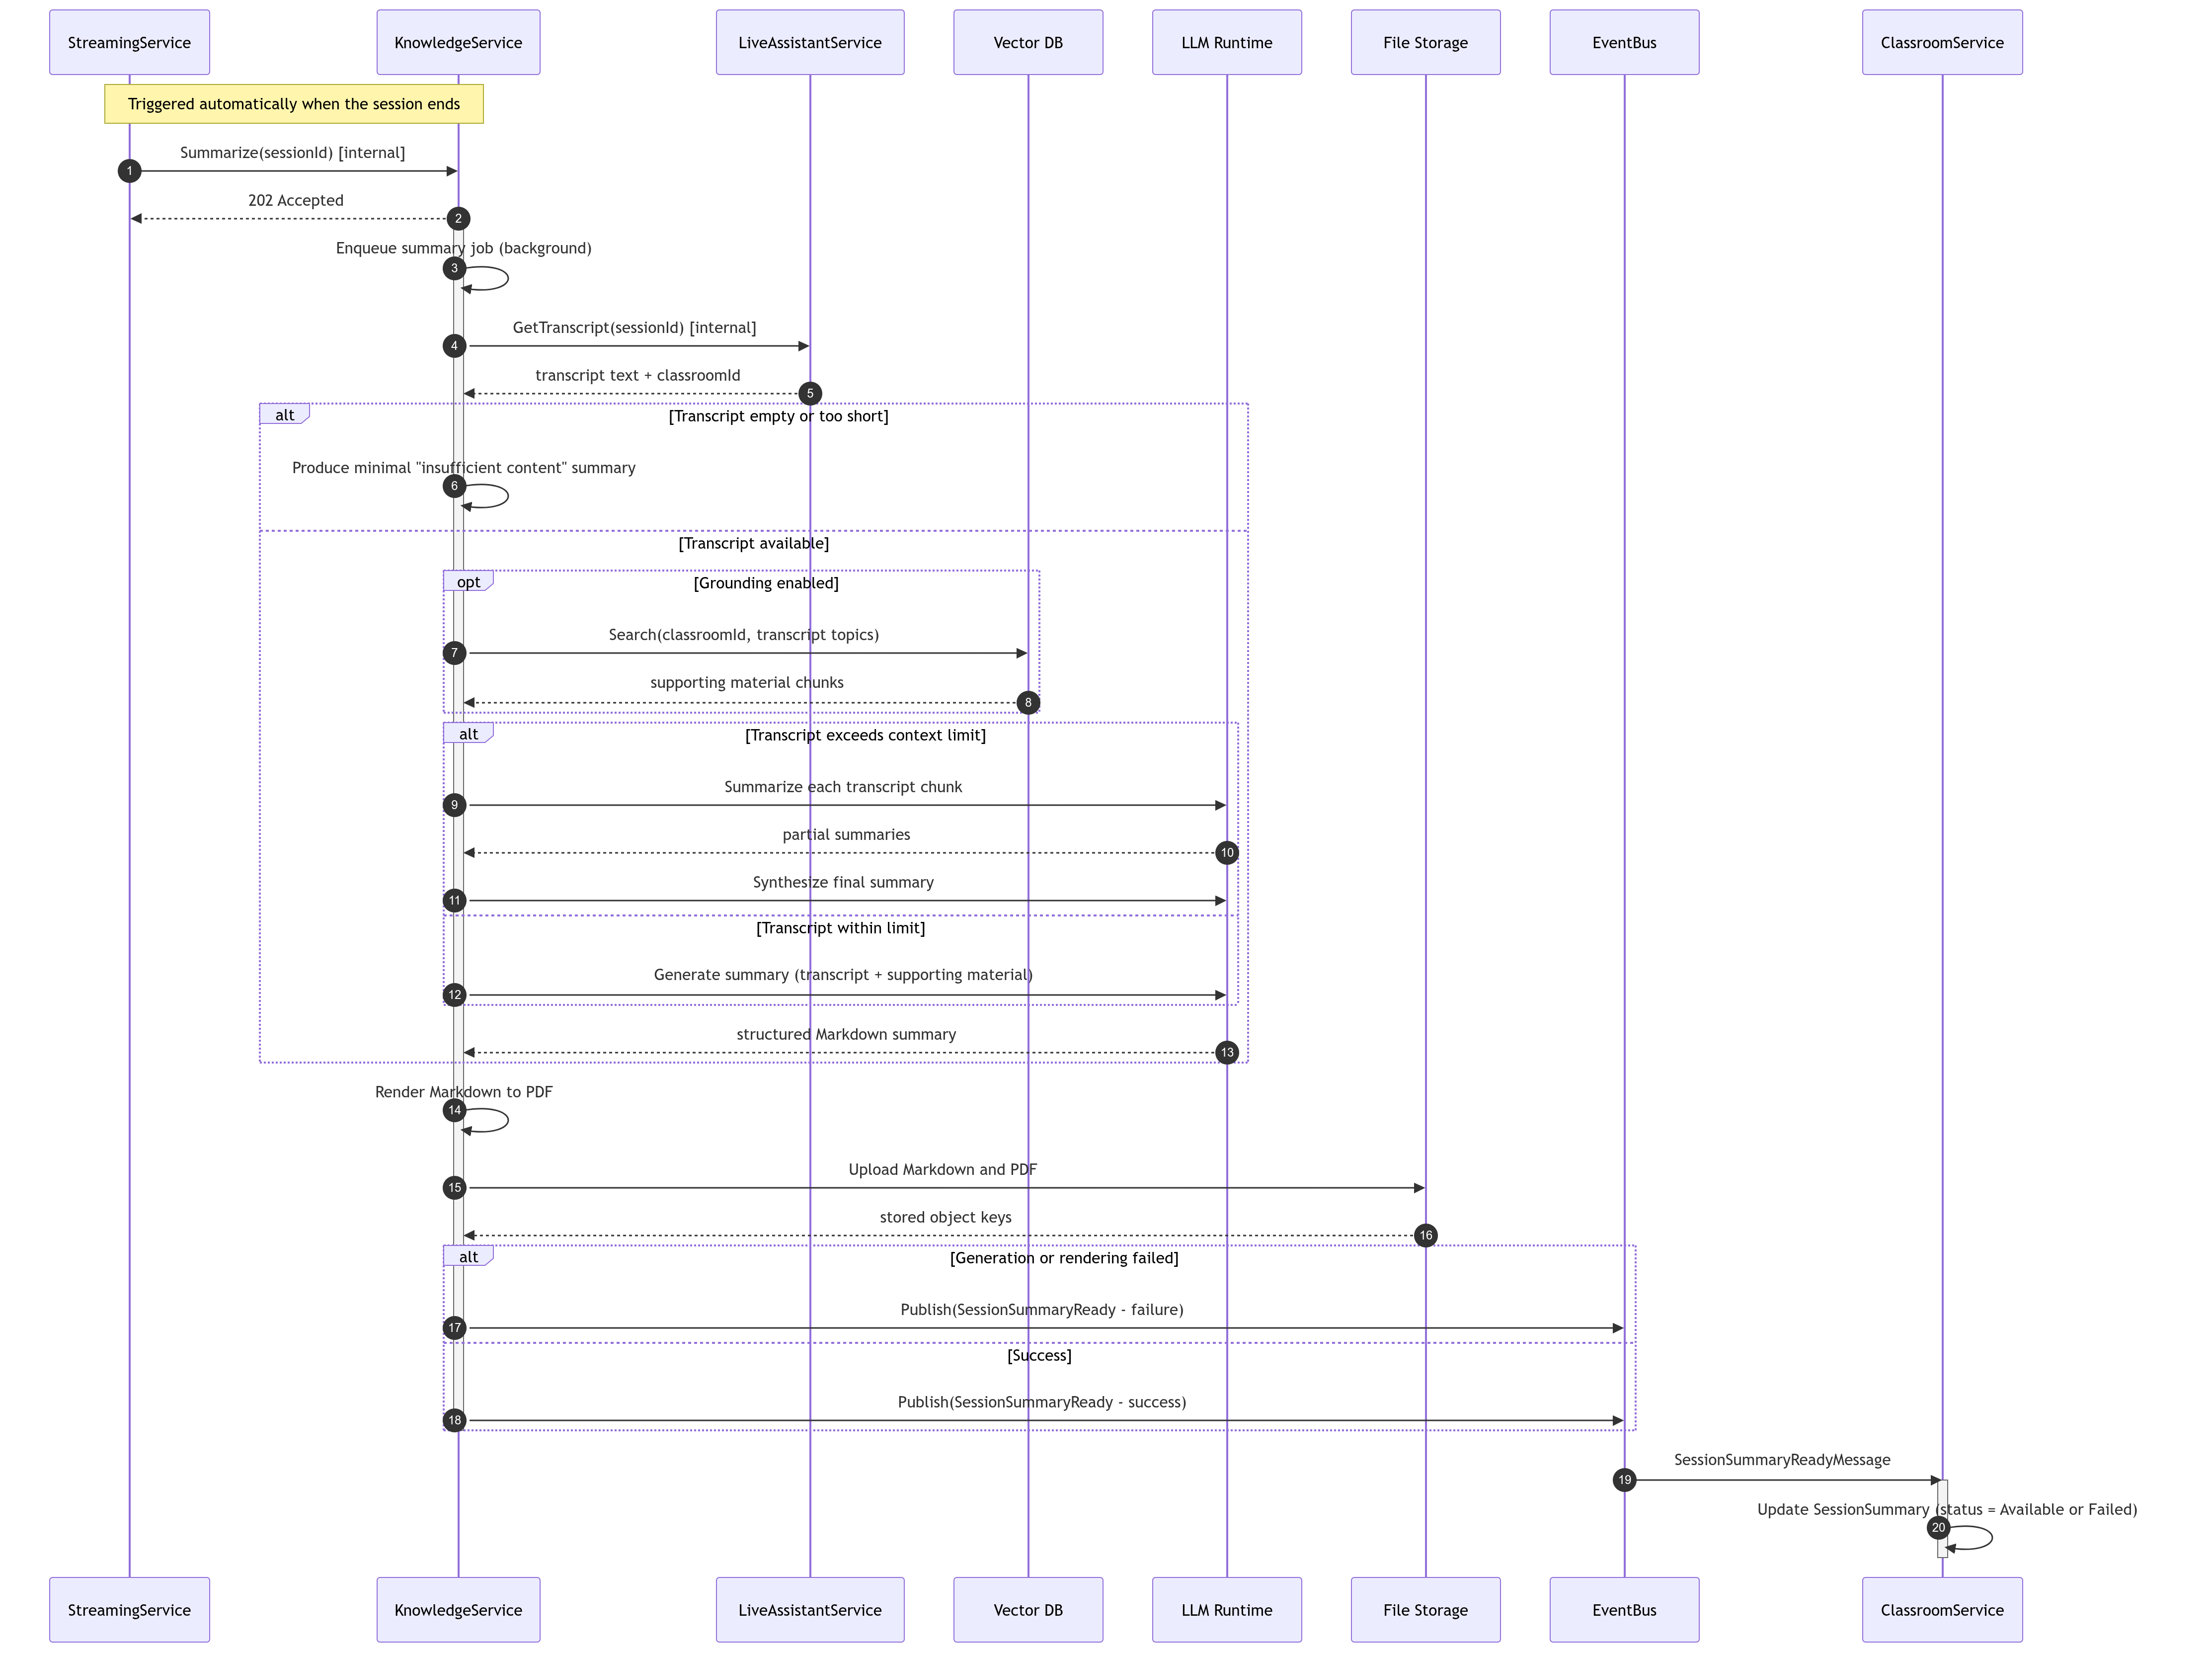
\includegraphics[width=\textwidth,height=0.8\textheight,keepaspectratio]{figures/image35.png}
  \caption{مخطط تسلسل النظام لحالة «توليد ملخّص الجلسة»: يوضّح الرسائل المتبادلة بين الفاعل والنظام بوصفه صندوقًا أسود، أي دون إظهار الخدمات الداخلية التي تنفّذها.}
  \label{fig:image35}
\end{figure}

\subsubsection{مخطط تسلسل النظام لحالة معاينة أثر حذف جلسة}

\begin{figure}[htbp]
  \centering
  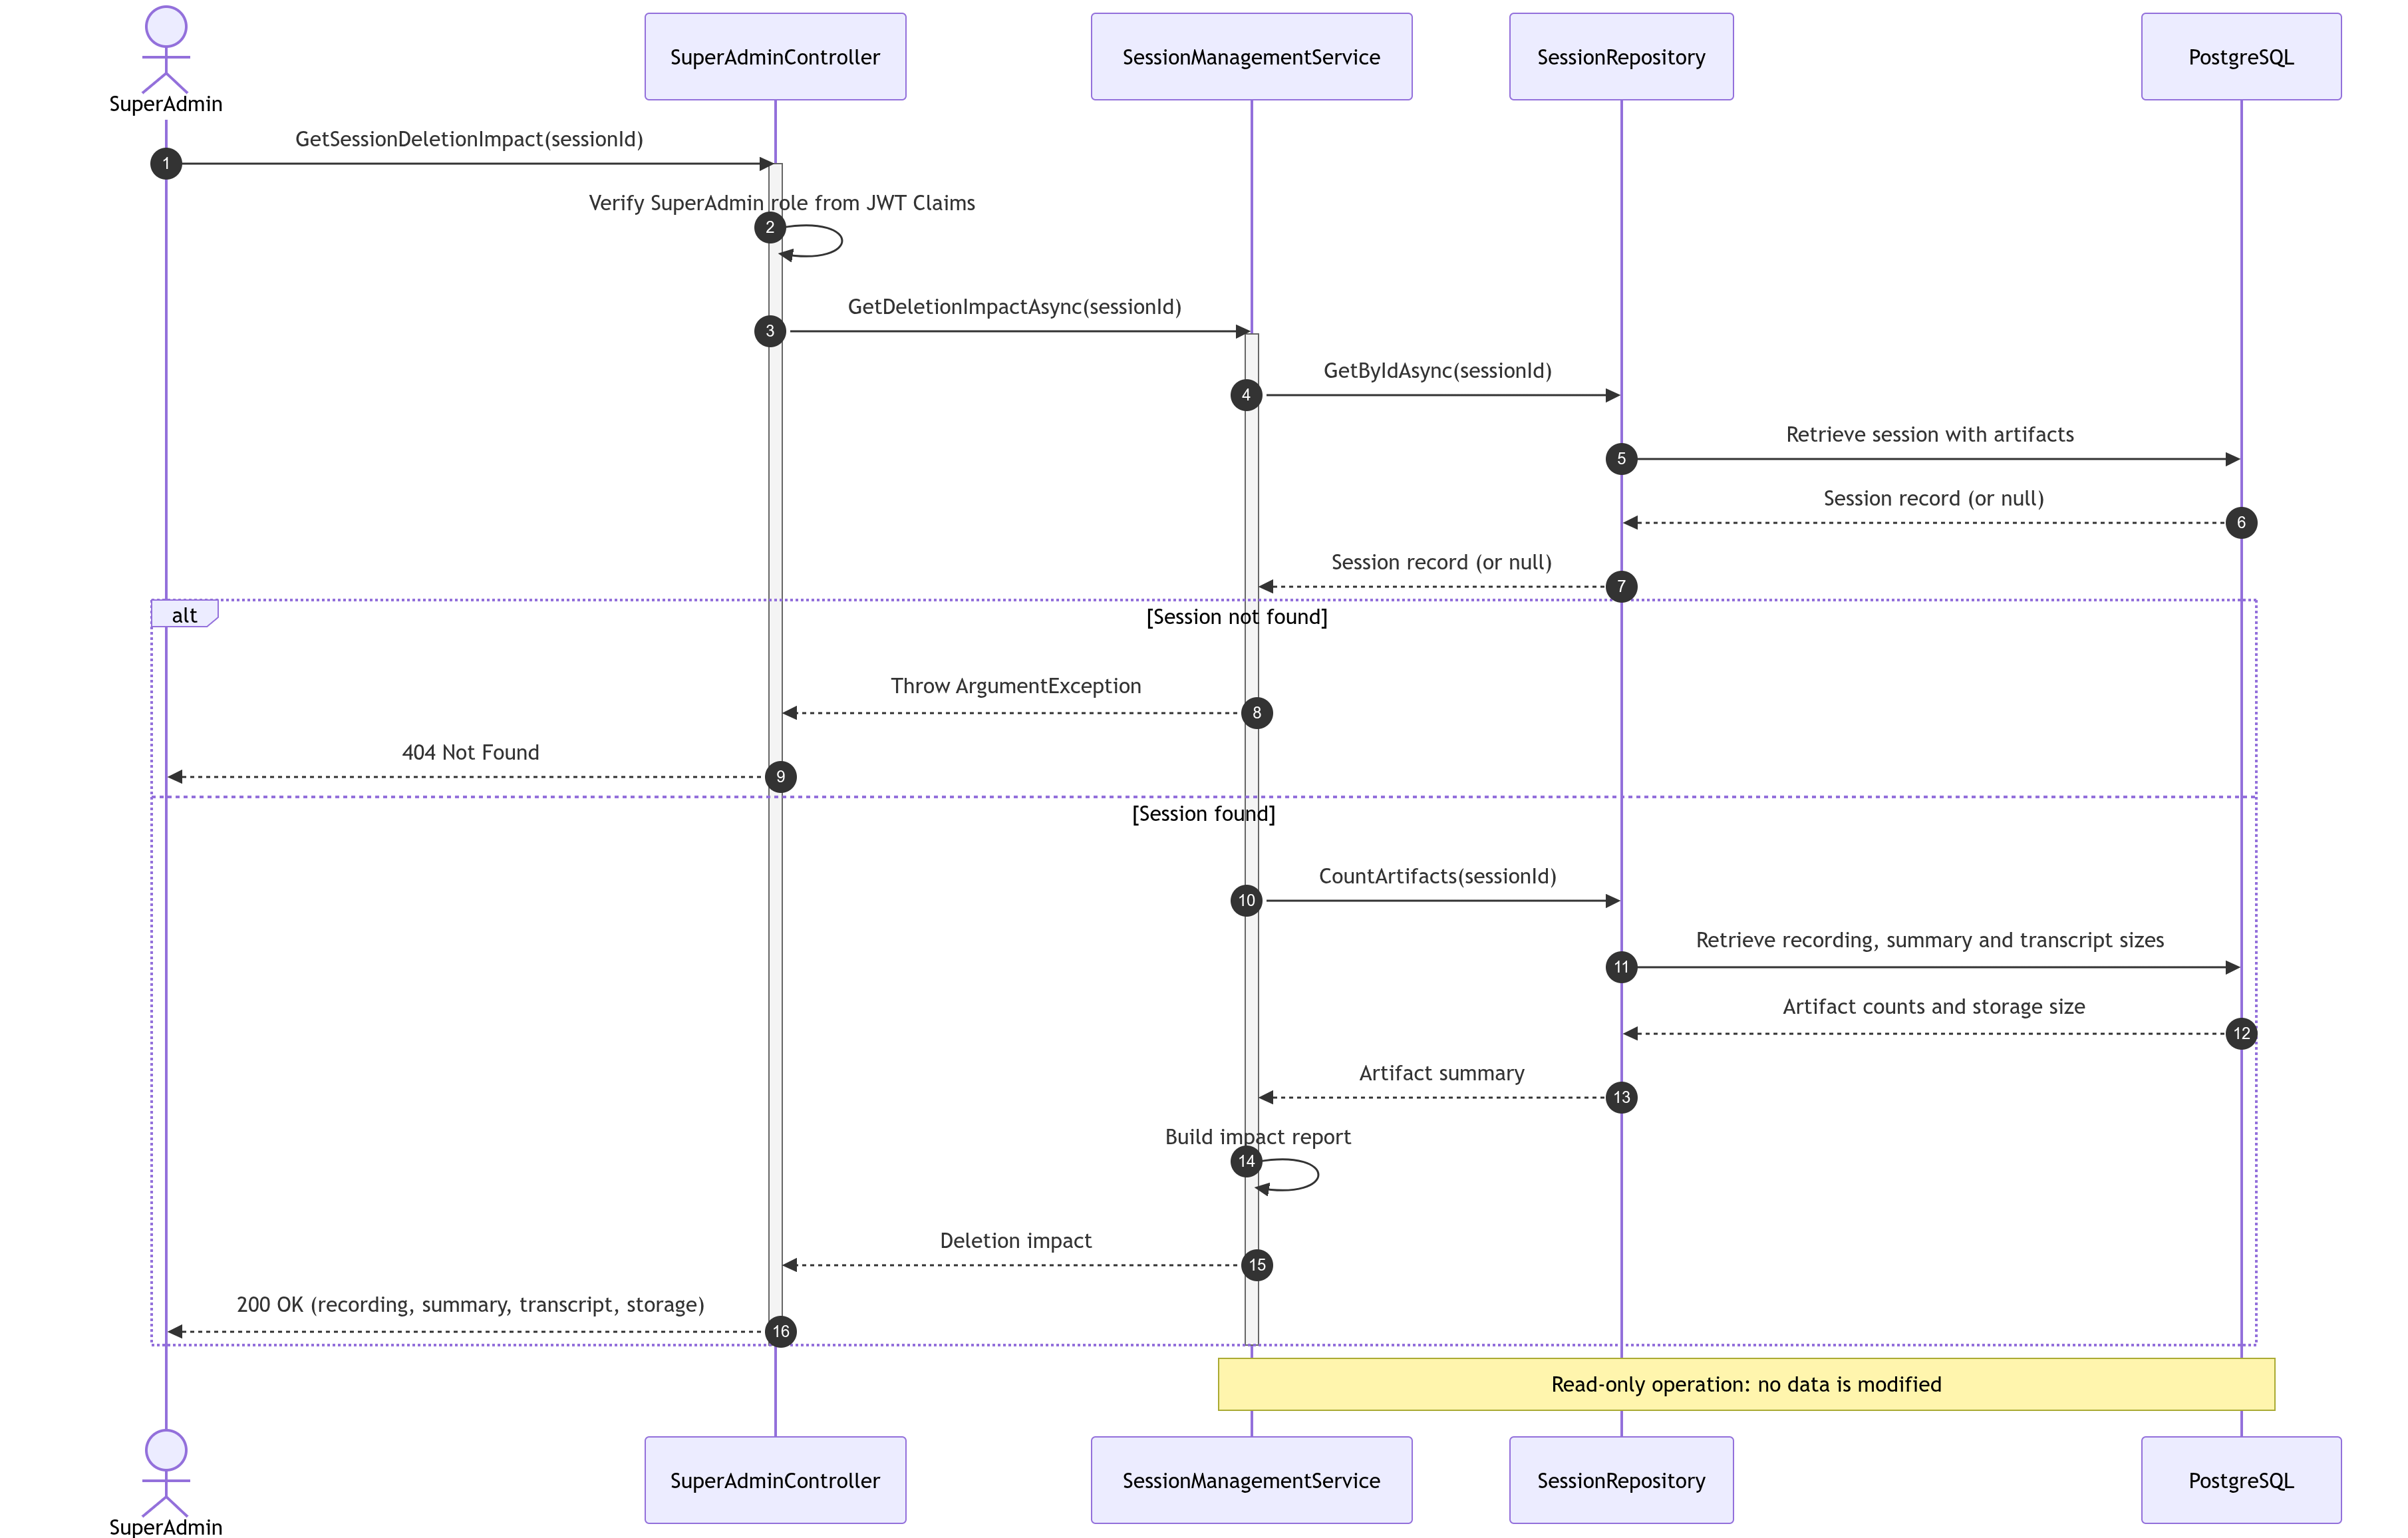
\includegraphics[width=\textwidth,height=0.8\textheight,keepaspectratio]{figures/image36.png}
  \caption{مخطط تسلسل النظام لحالة «معاينة أثر حذف جلسة»: يوضّح الرسائل المتبادلة بين الفاعل والنظام بوصفه صندوقًا أسود، أي دون إظهار الخدمات الداخلية التي تنفّذها.}
  \label{fig:image36}
\end{figure}

\subsubsection{مخطط تسلسل النظام لحالة حذف جلسة ومخرجاتها}

\begin{figure}[htbp]
  \centering
  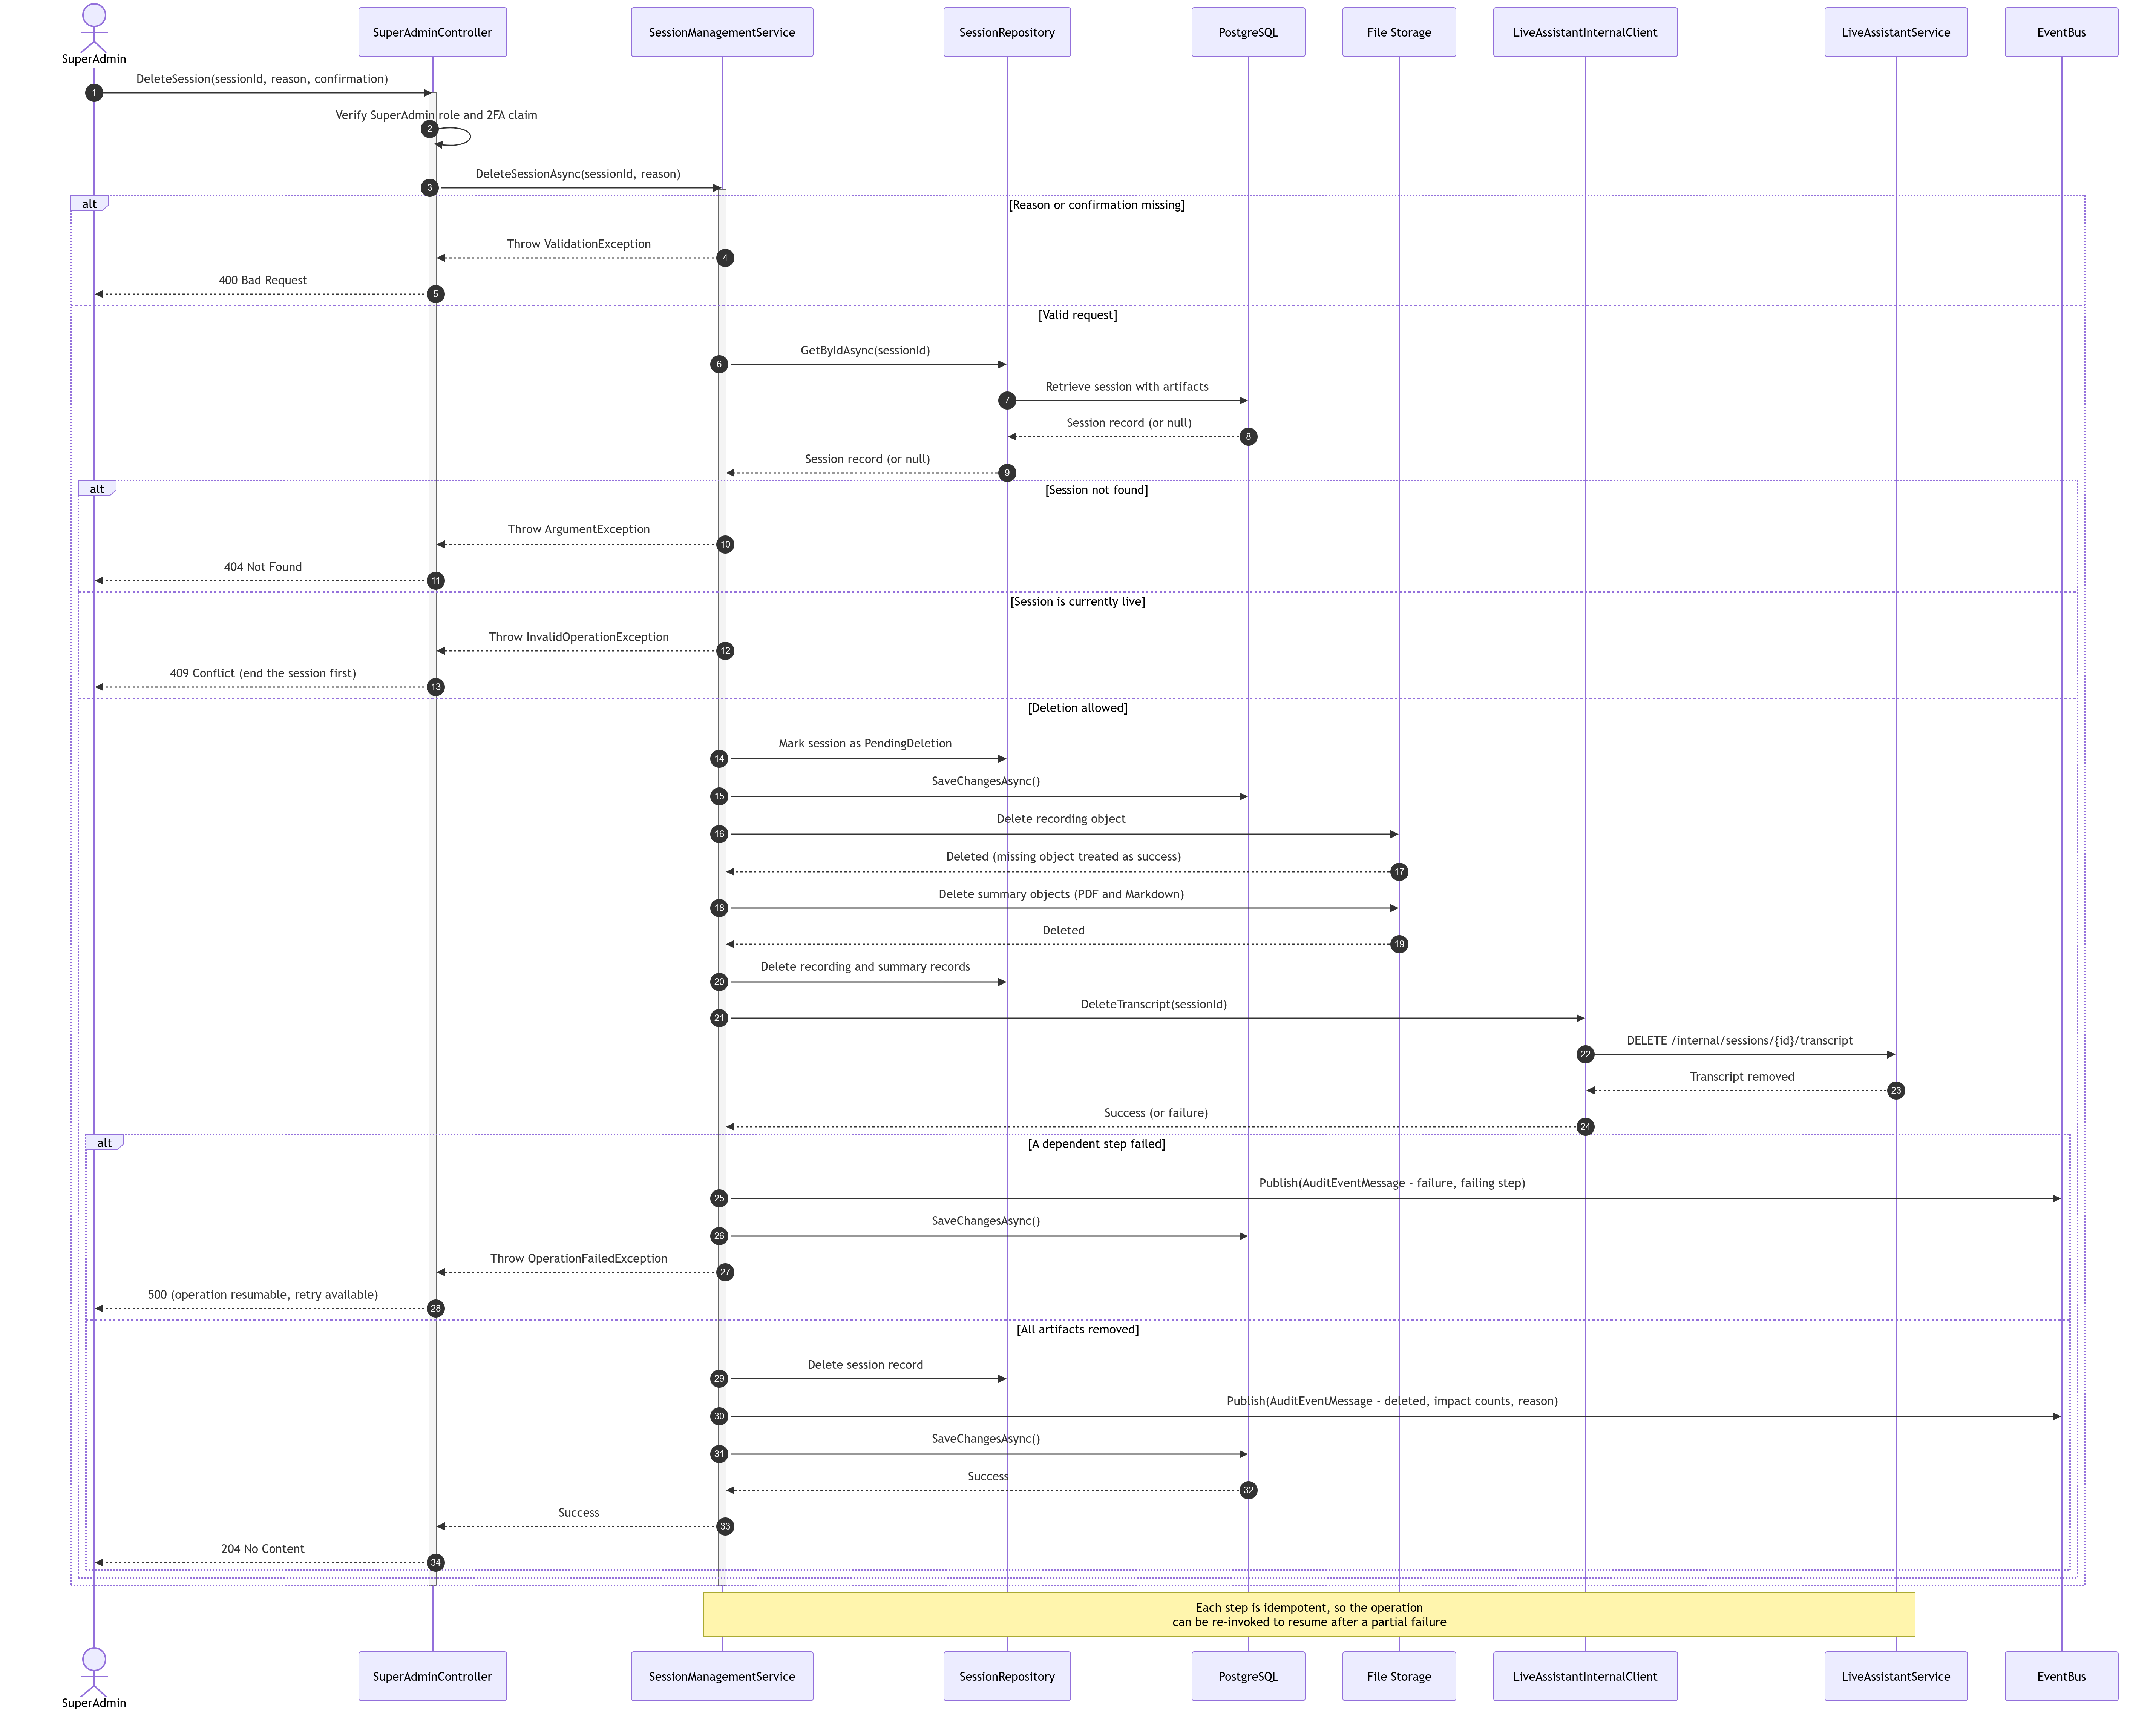
\includegraphics[width=\textwidth,height=0.8\textheight,keepaspectratio]{figures/image37.png}
  \caption{مخطط تسلسل النظام لحالة «حذف جلسة ومخرجاتها»: يوضّح الرسائل المتبادلة بين الفاعل والنظام بوصفه صندوقًا أسود، أي دون إظهار الخدمات الداخلية التي تنفّذها.}
  \label{fig:image37}
\end{figure}

\subsubsection{مخطط تسلسل النظام لحالة استعراض الملفات وحالة فهرستها}

\begin{figure}[htbp]
  \centering
  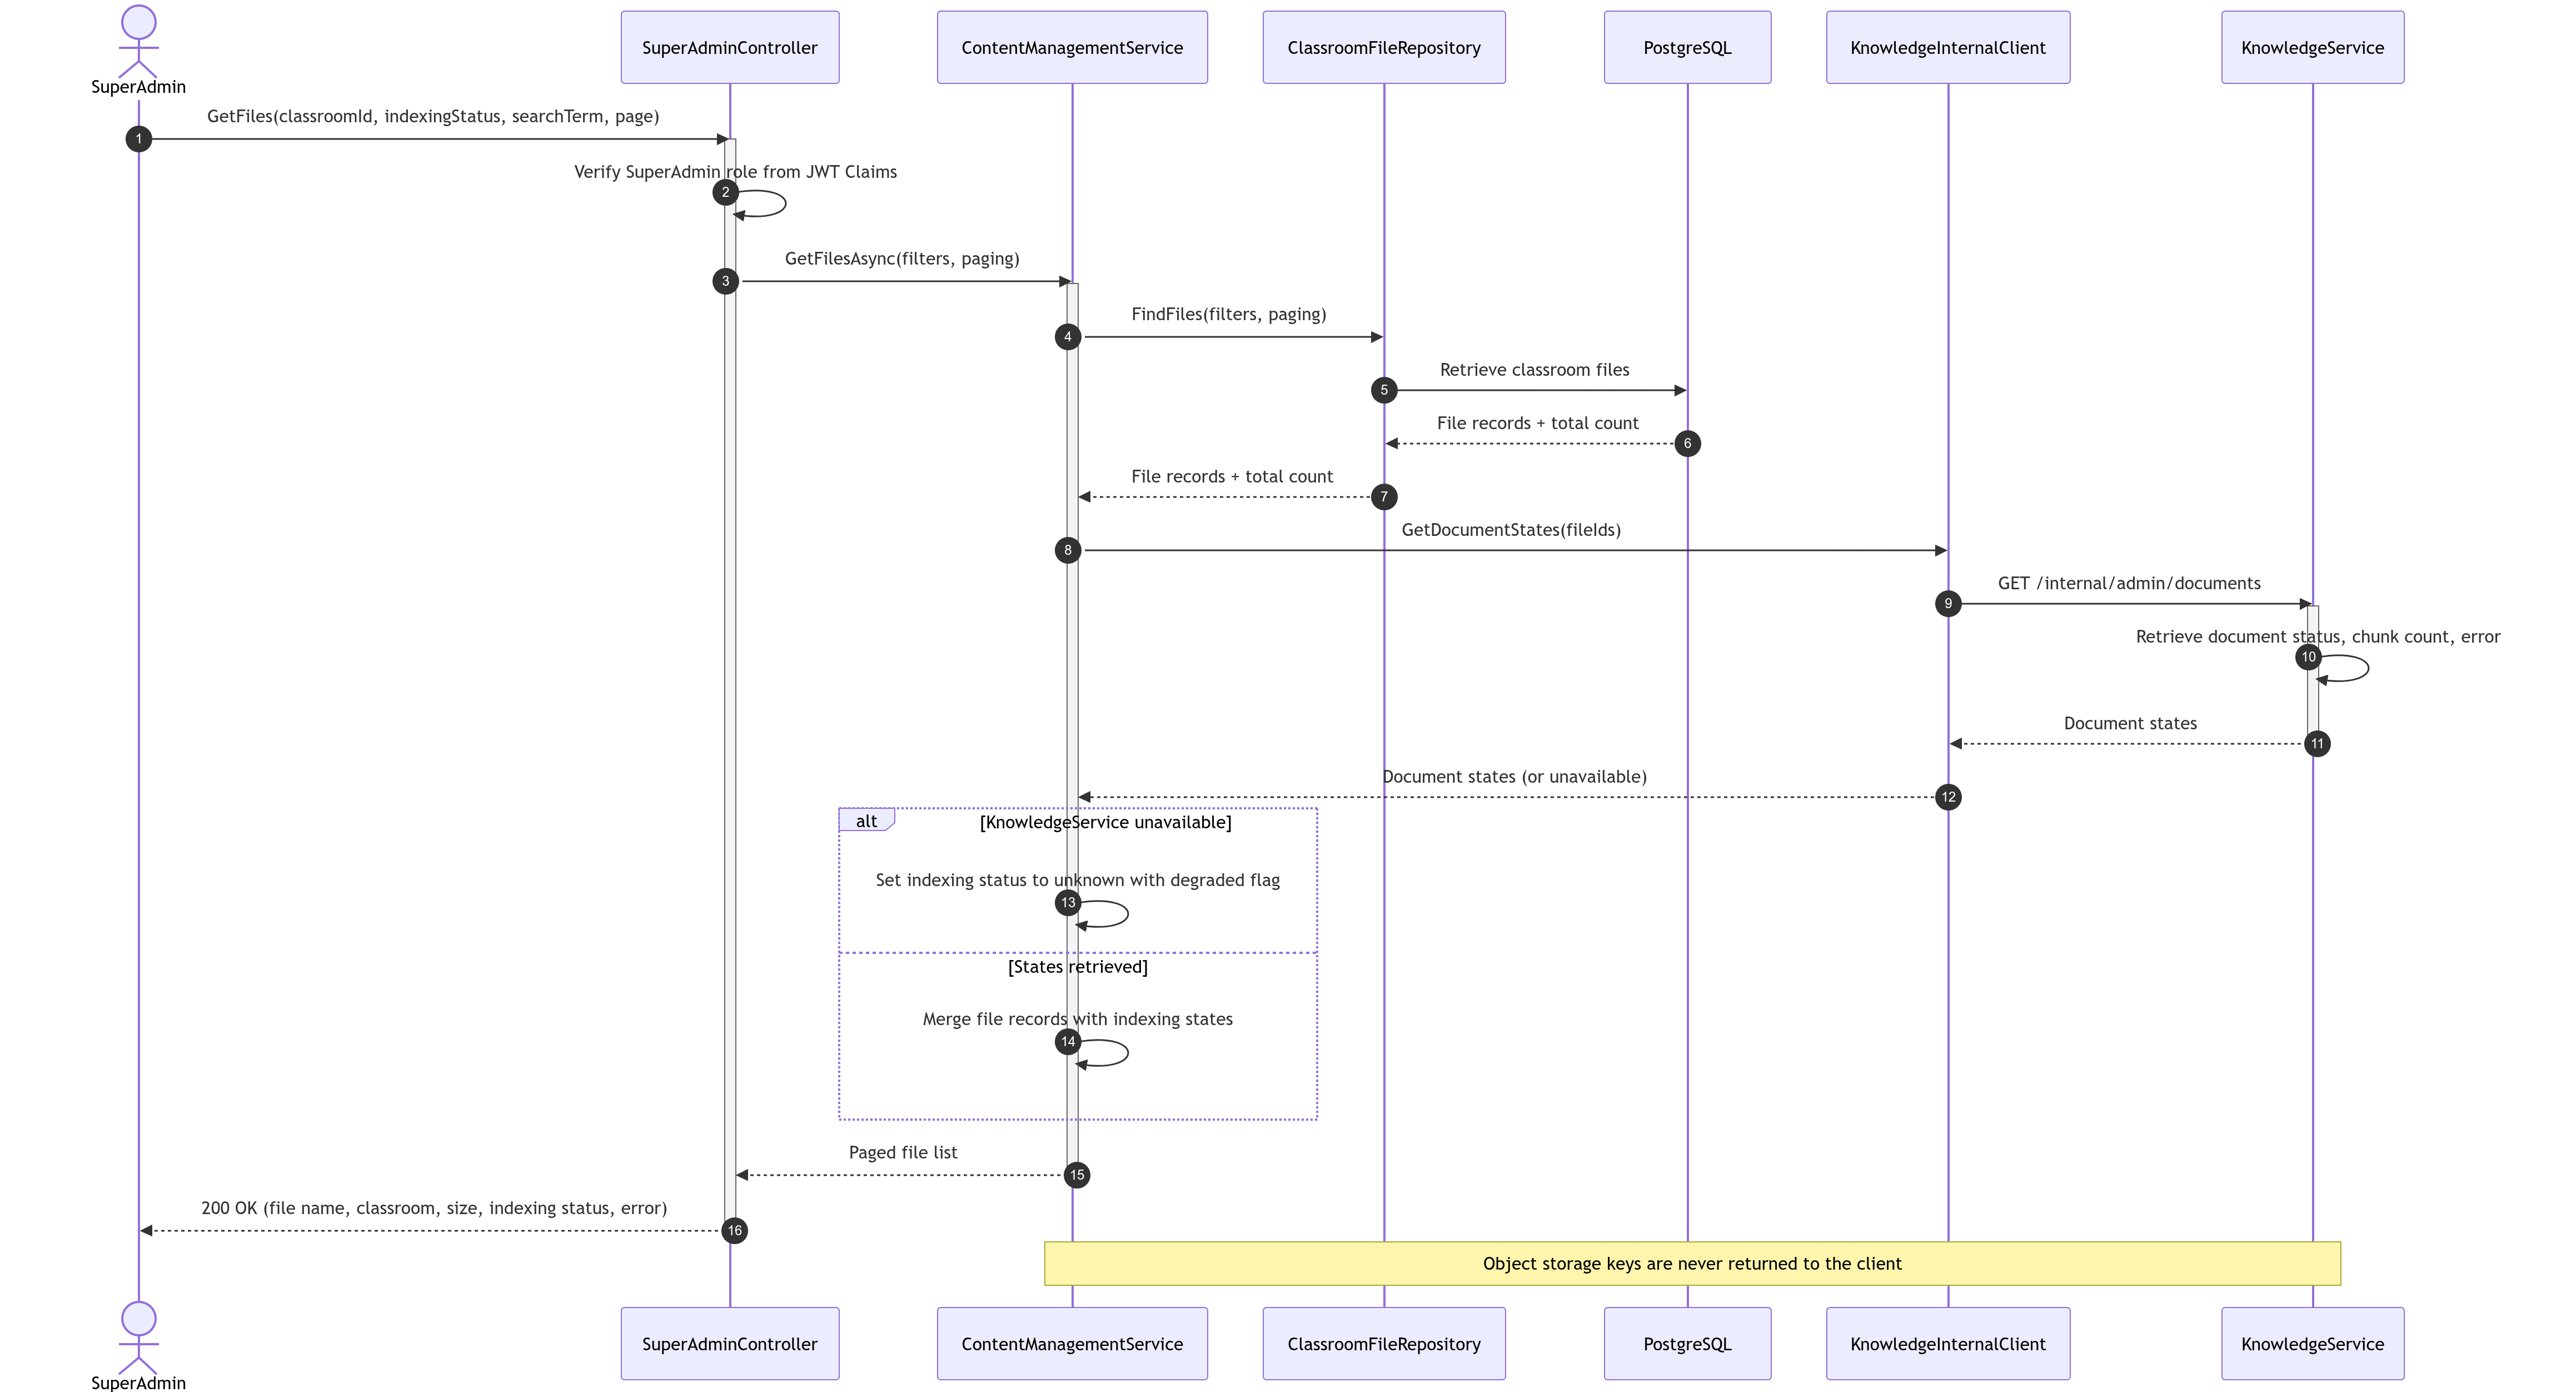
\includegraphics[width=\textwidth,height=0.8\textheight,keepaspectratio]{figures/image38.png}
  \caption{مخطط تسلسل النظام لحالة «استعراض الملفات وحالة فهرستها»: يوضّح الرسائل المتبادلة بين الفاعل والنظام بوصفه صندوقًا أسود، أي دون إظهار الخدمات الداخلية التي تنفّذها.}
  \label{fig:image38}
\end{figure}

\subsubsection{مخطط تسلسل النظام لحالة استعراض إحصائيات قاعدة المعرفة}

\begin{figure}[htbp]
  \centering
  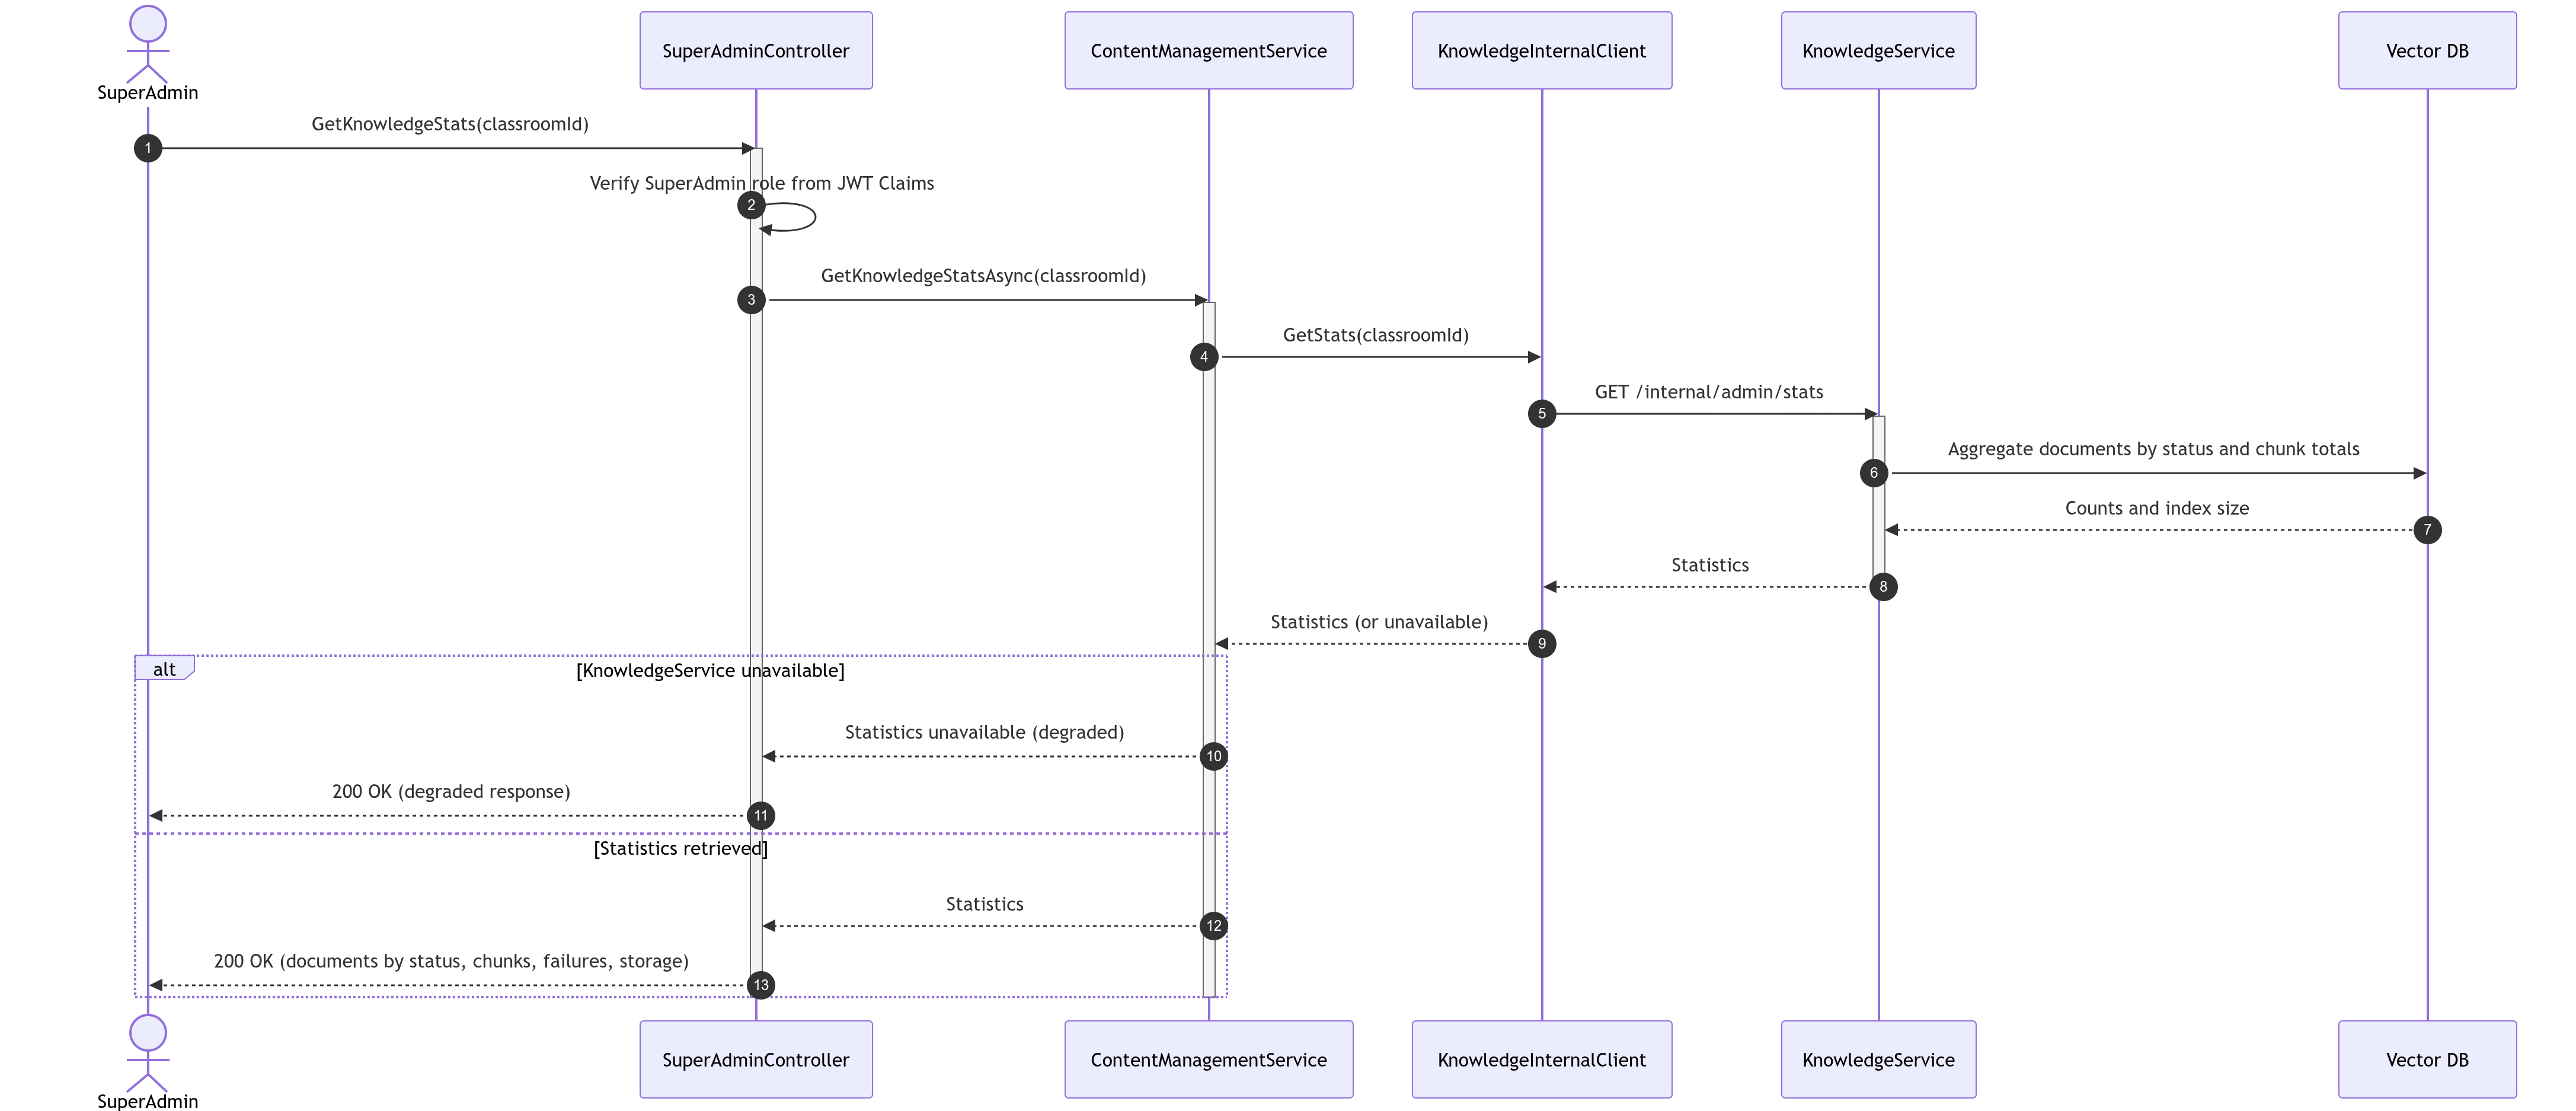
\includegraphics[width=\textwidth,height=0.8\textheight,keepaspectratio]{figures/image39.png}
  \caption{مخطط تسلسل النظام لحالة «استعراض إحصائيات قاعدة المعرفة»: يوضّح الرسائل المتبادلة بين الفاعل والنظام بوصفه صندوقًا أسود، أي دون إظهار الخدمات الداخلية التي تنفّذها.}
  \label{fig:image39}
\end{figure}

\subsubsection{مخطط تسلسل النظام لحالة إعادة فهرسة ملف أو ملفات فصل دراسي}

\begin{figure}[htbp]
  \centering
  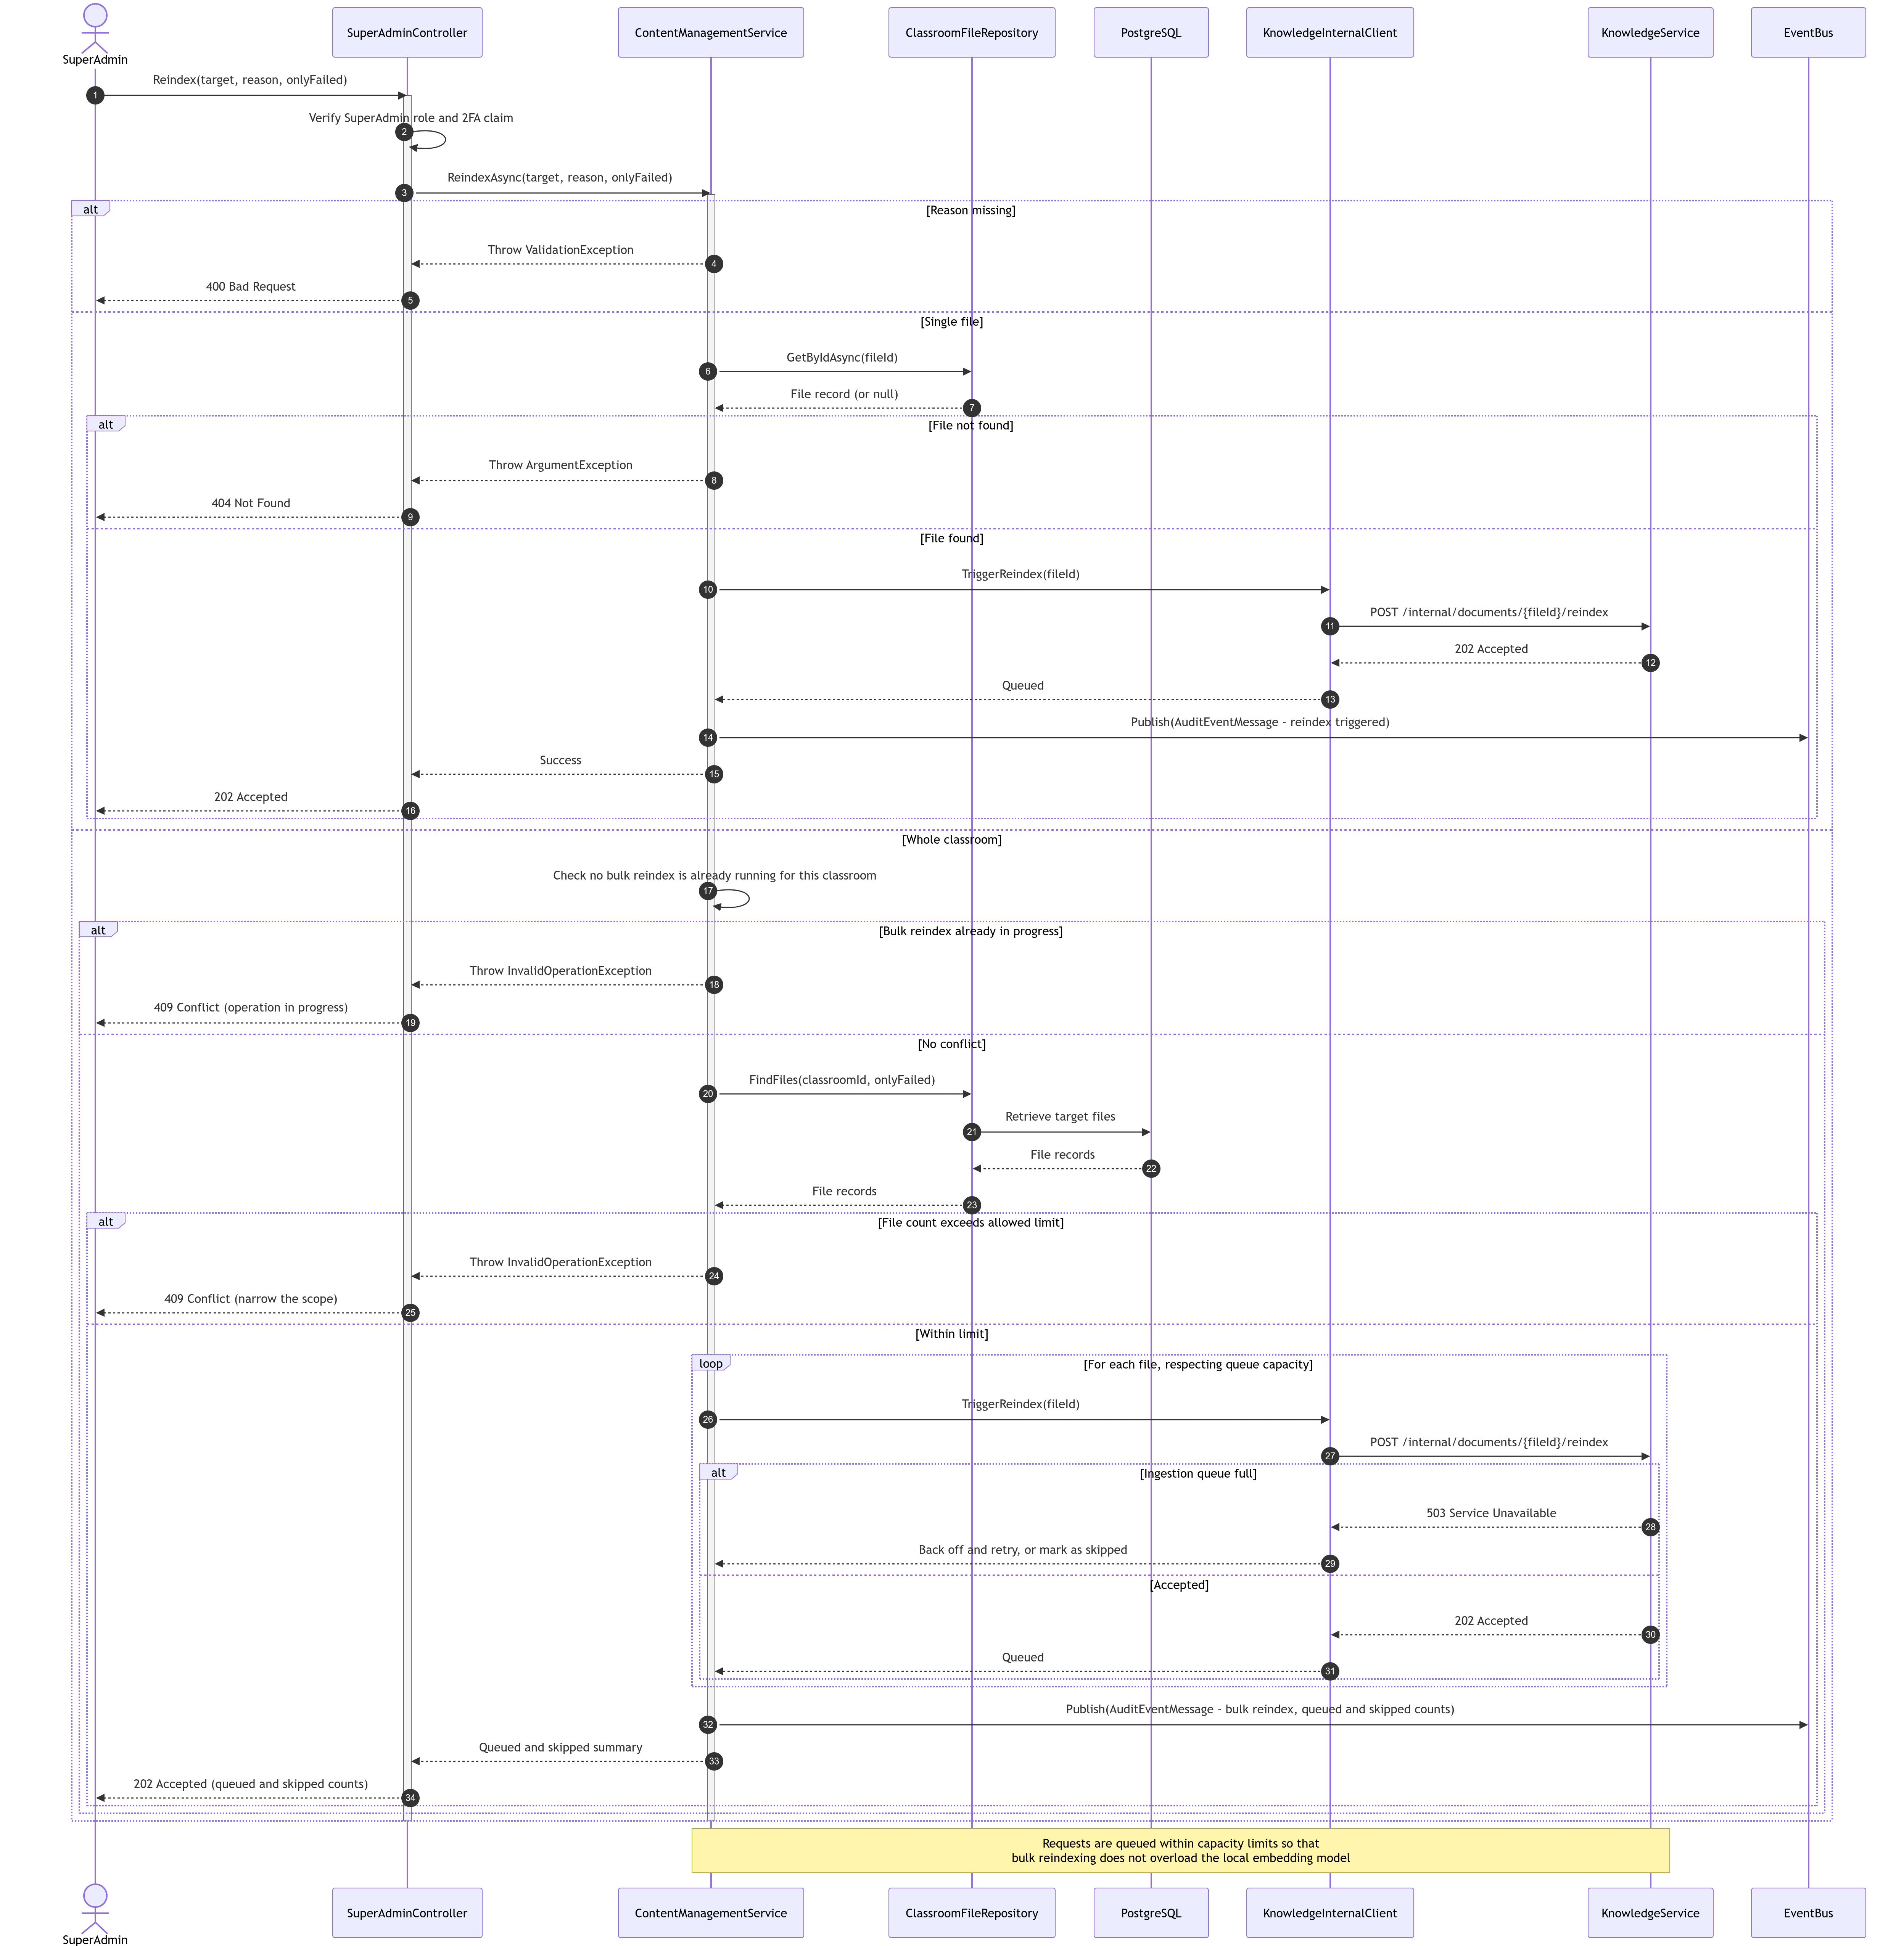
\includegraphics[width=\textwidth,height=0.8\textheight,keepaspectratio]{figures/image40.png}
  \caption{مخطط تسلسل النظام لحالة «إعادة فهرسة ملف أو ملفات فصل دراسي»: يوضّح الرسائل المتبادلة بين الفاعل والنظام بوصفه صندوقًا أسود، أي دون إظهار الخدمات الداخلية التي تنفّذها.}
  \label{fig:image40}
\end{figure}

\subsubsection{مخطط تسلسل النظام لحالة حذف ملف مع مقاطعه المفهرسة}

\begin{figure}[htbp]
  \centering
  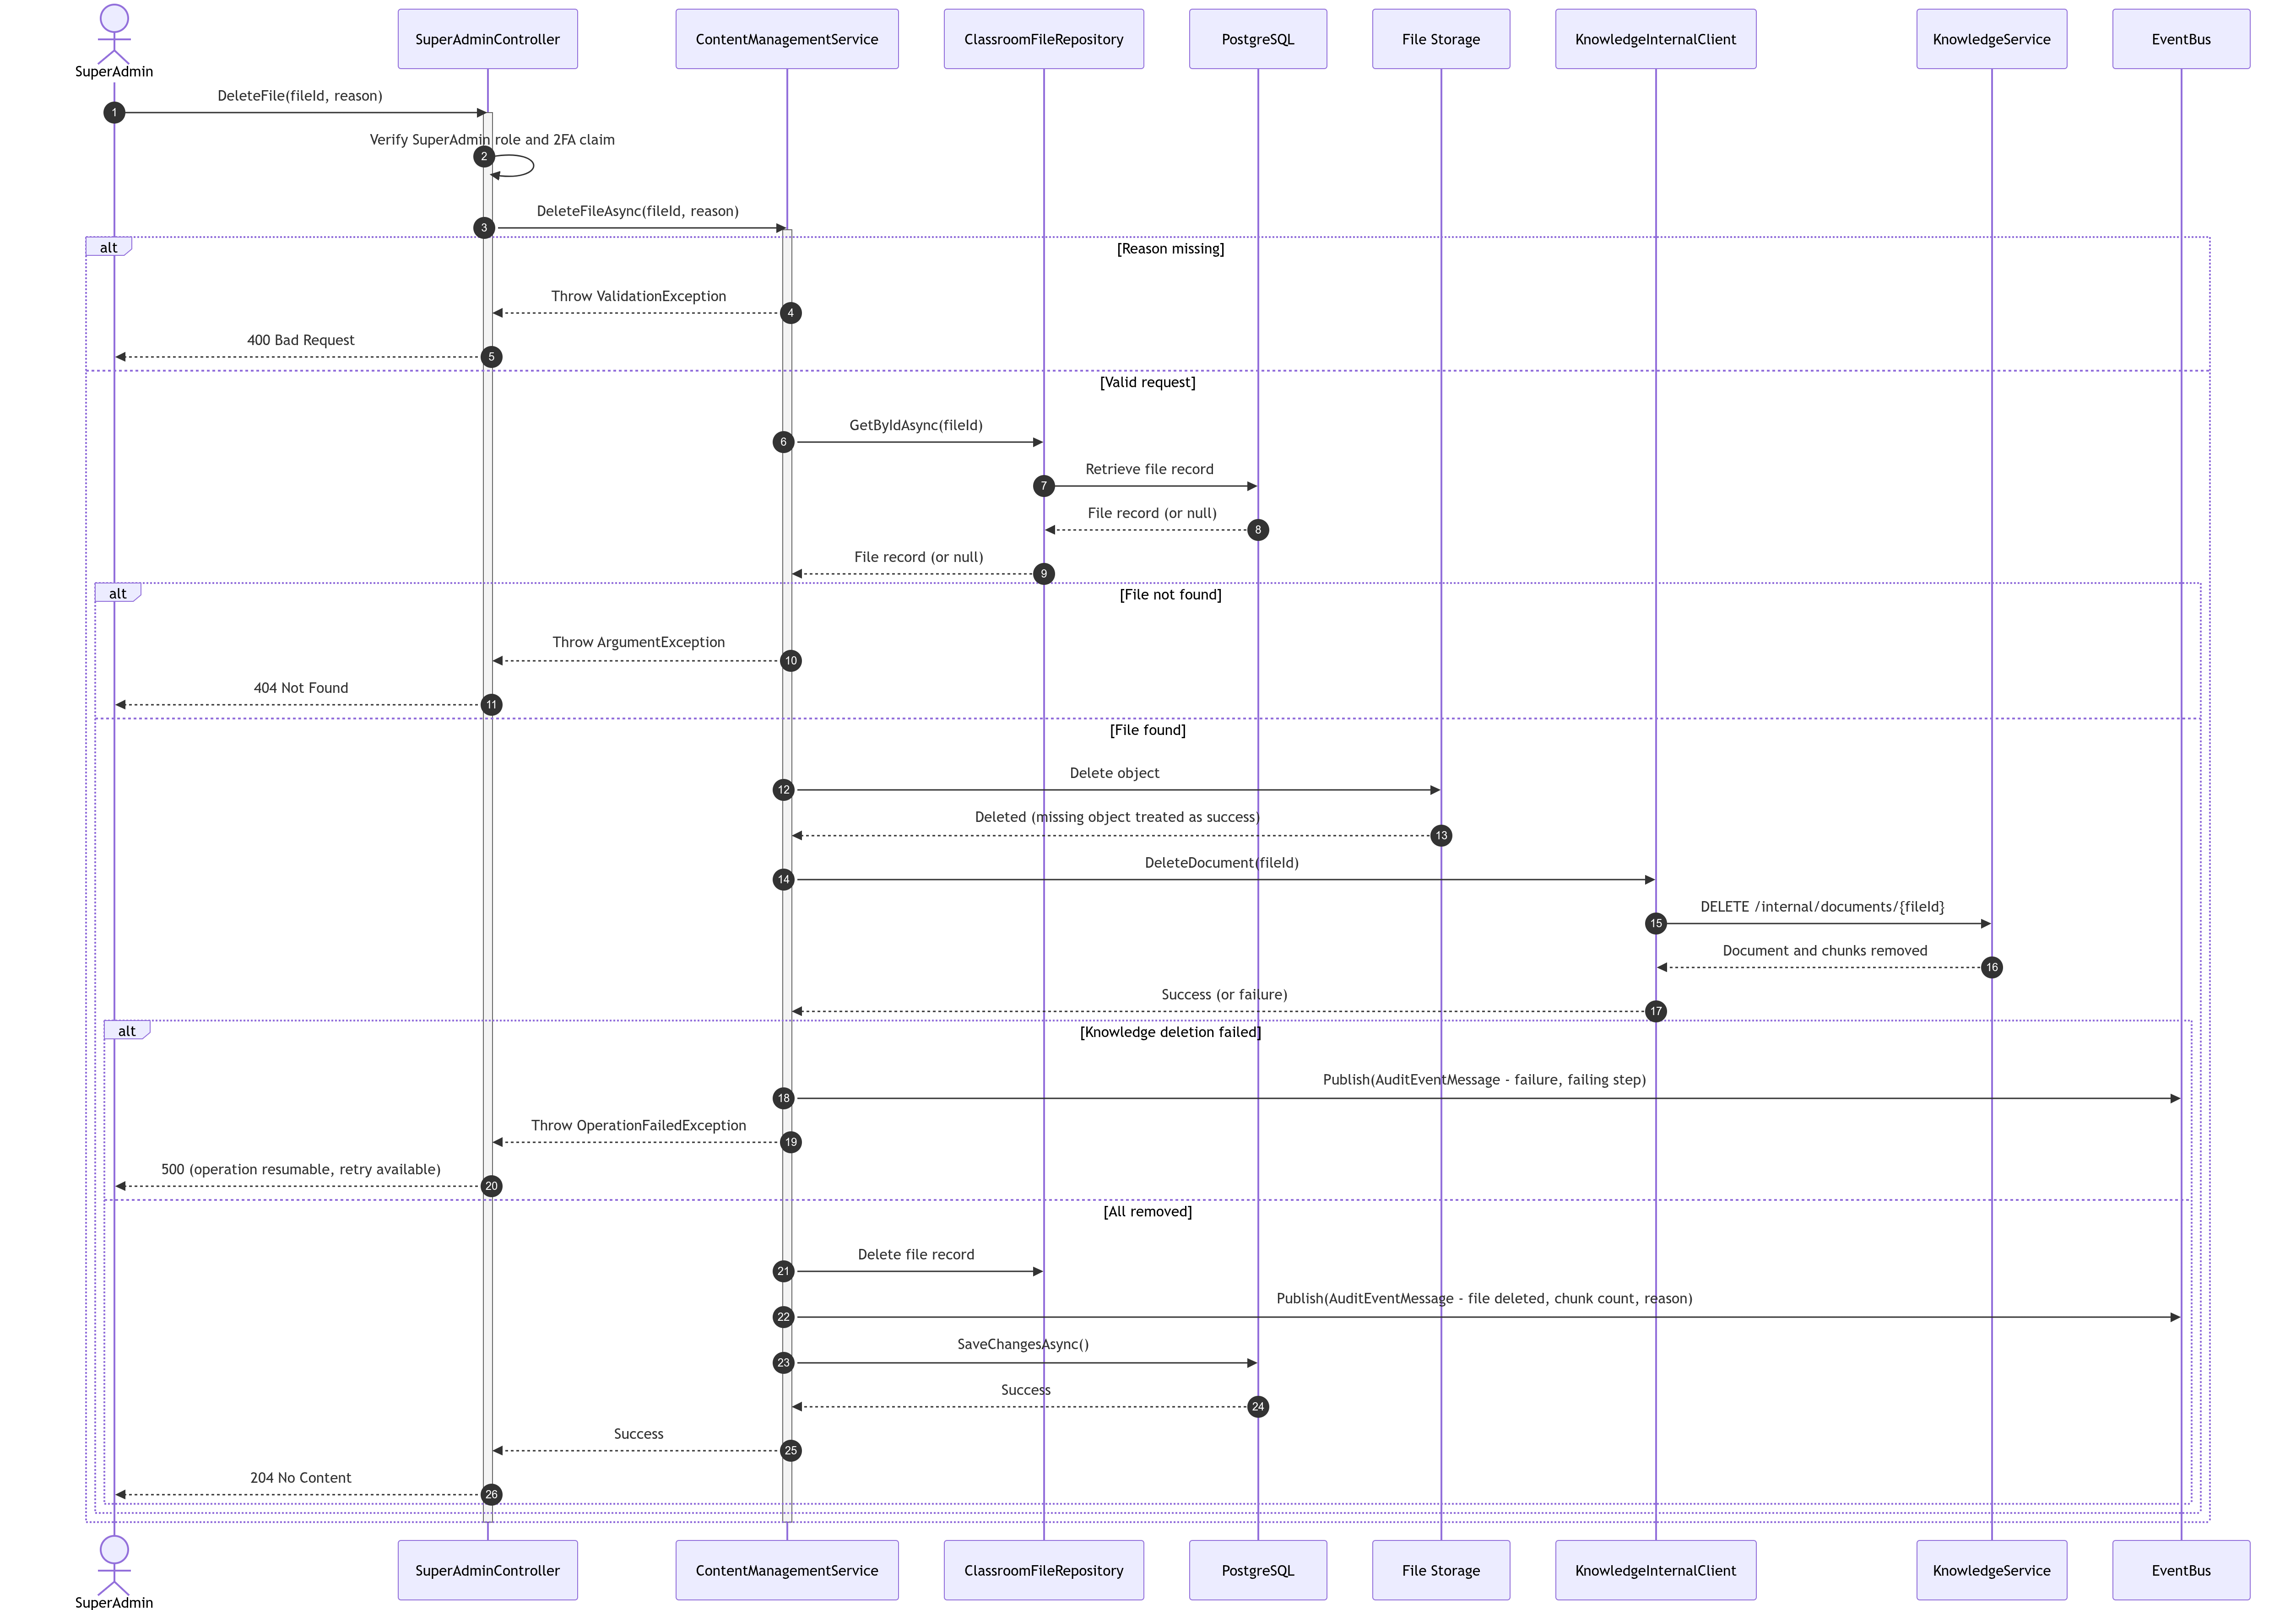
\includegraphics[width=\textwidth,height=0.8\textheight,keepaspectratio]{figures/image41.png}
  \caption{مخطط تسلسل النظام لحالة «حذف ملف مع مقاطعه المفهرسة»: يوضّح الرسائل المتبادلة بين الفاعل والنظام بوصفه صندوقًا أسود، أي دون إظهار الخدمات الداخلية التي تنفّذها.}
  \label{fig:image41}
\end{figure}

\subsubsection{مخطط تسلسل النظام لحالة استعراض التسجيلات والملخصات وحالاتها}

\begin{figure}[htbp]
  \centering
  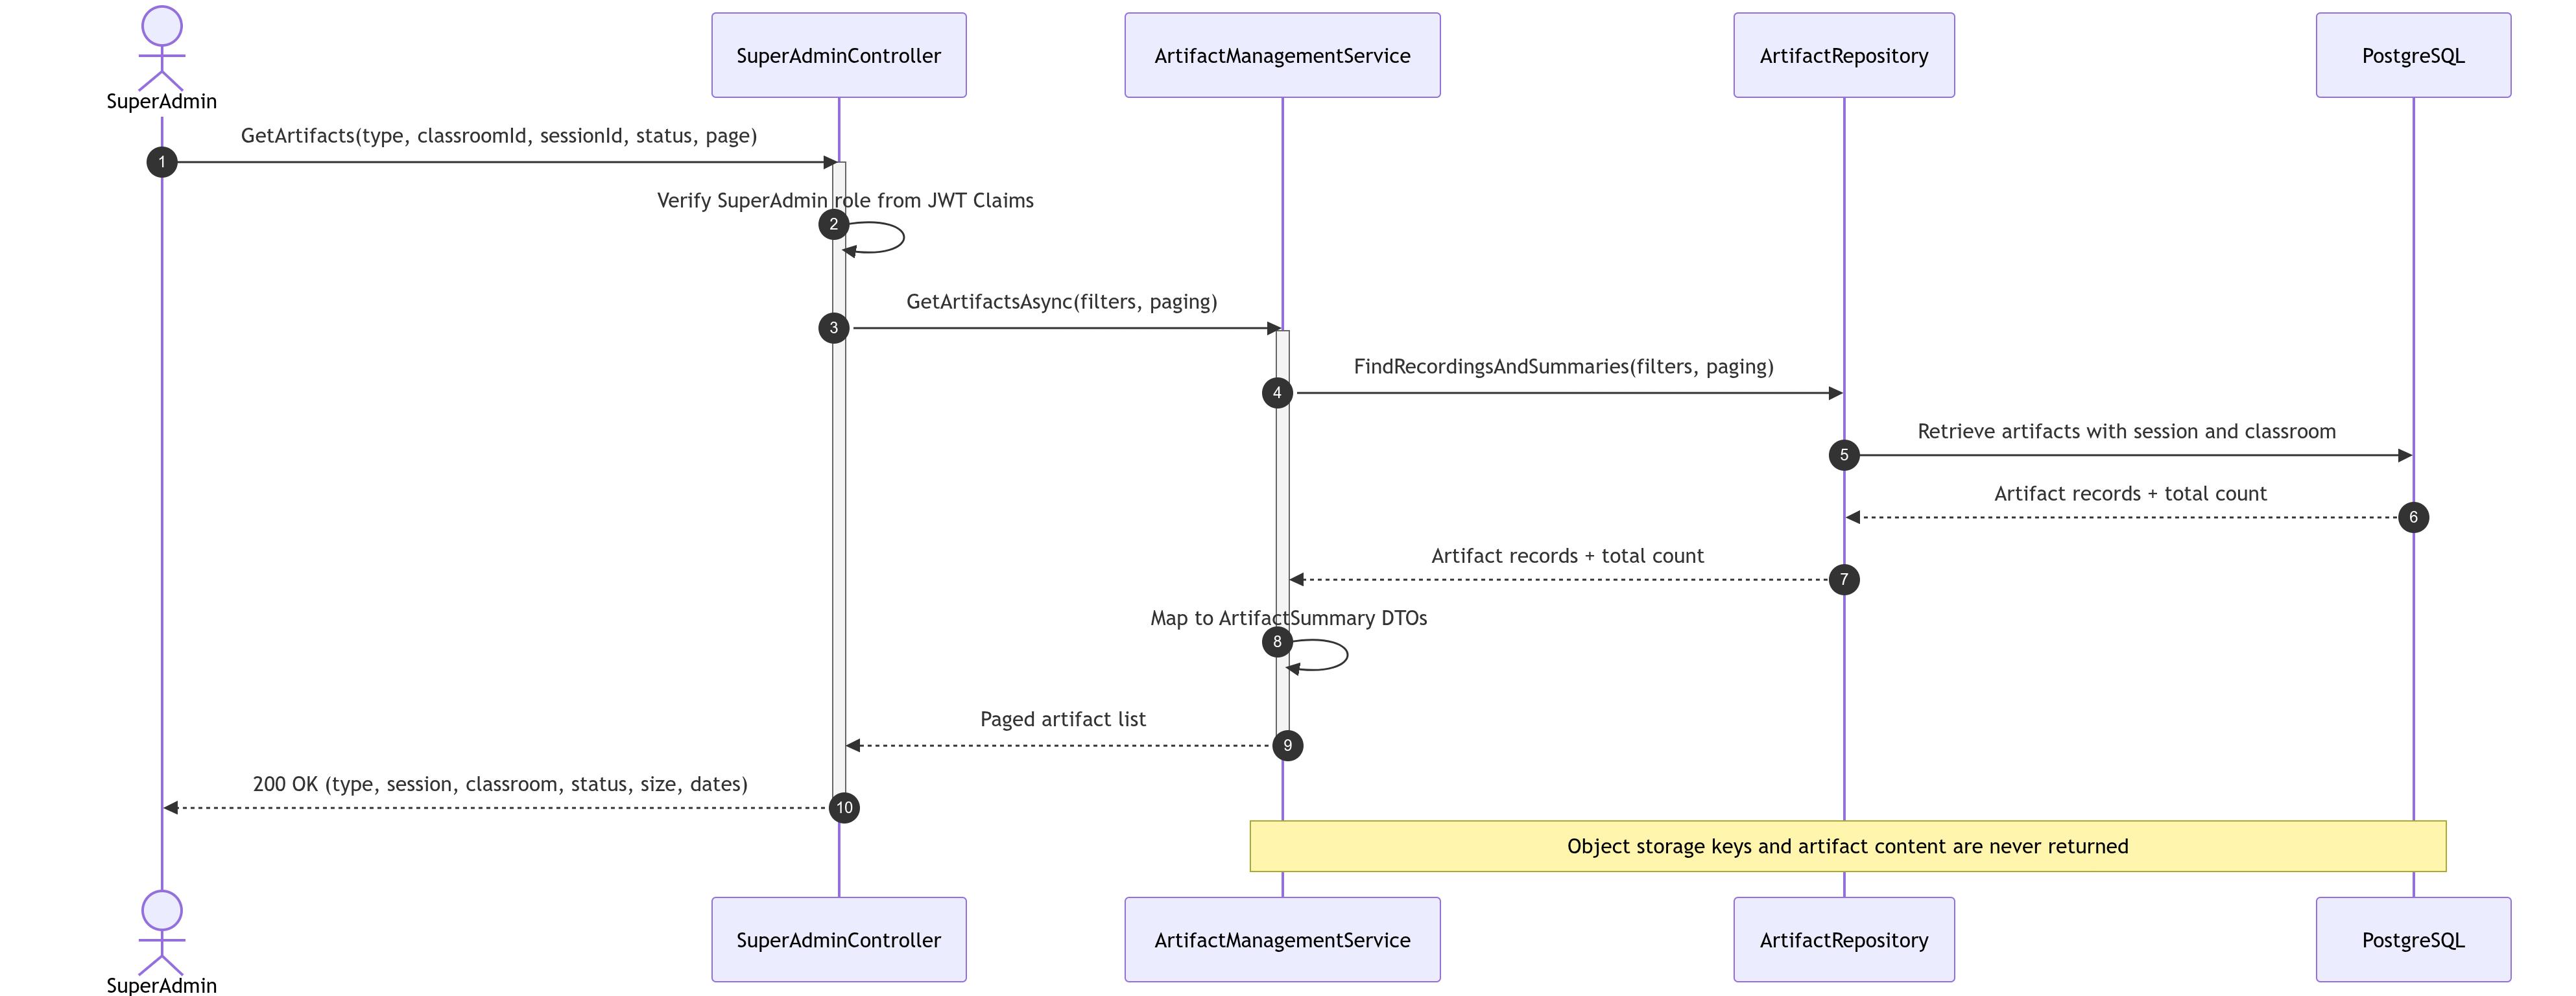
\includegraphics[width=\textwidth,height=0.8\textheight,keepaspectratio]{figures/image42.png}
  \caption{مخطط تسلسل النظام لحالة «استعراض التسجيلات والملخصات وحالاتها»: يوضّح الرسائل المتبادلة بين الفاعل والنظام بوصفه صندوقًا أسود، أي دون إظهار الخدمات الداخلية التي تنفّذها.}
  \label{fig:image42}
\end{figure}

\subsubsection{مخطط تسلسل النظام لحالة حذف تسجيل أو ملخص}

\begin{figure}[htbp]
  \centering
  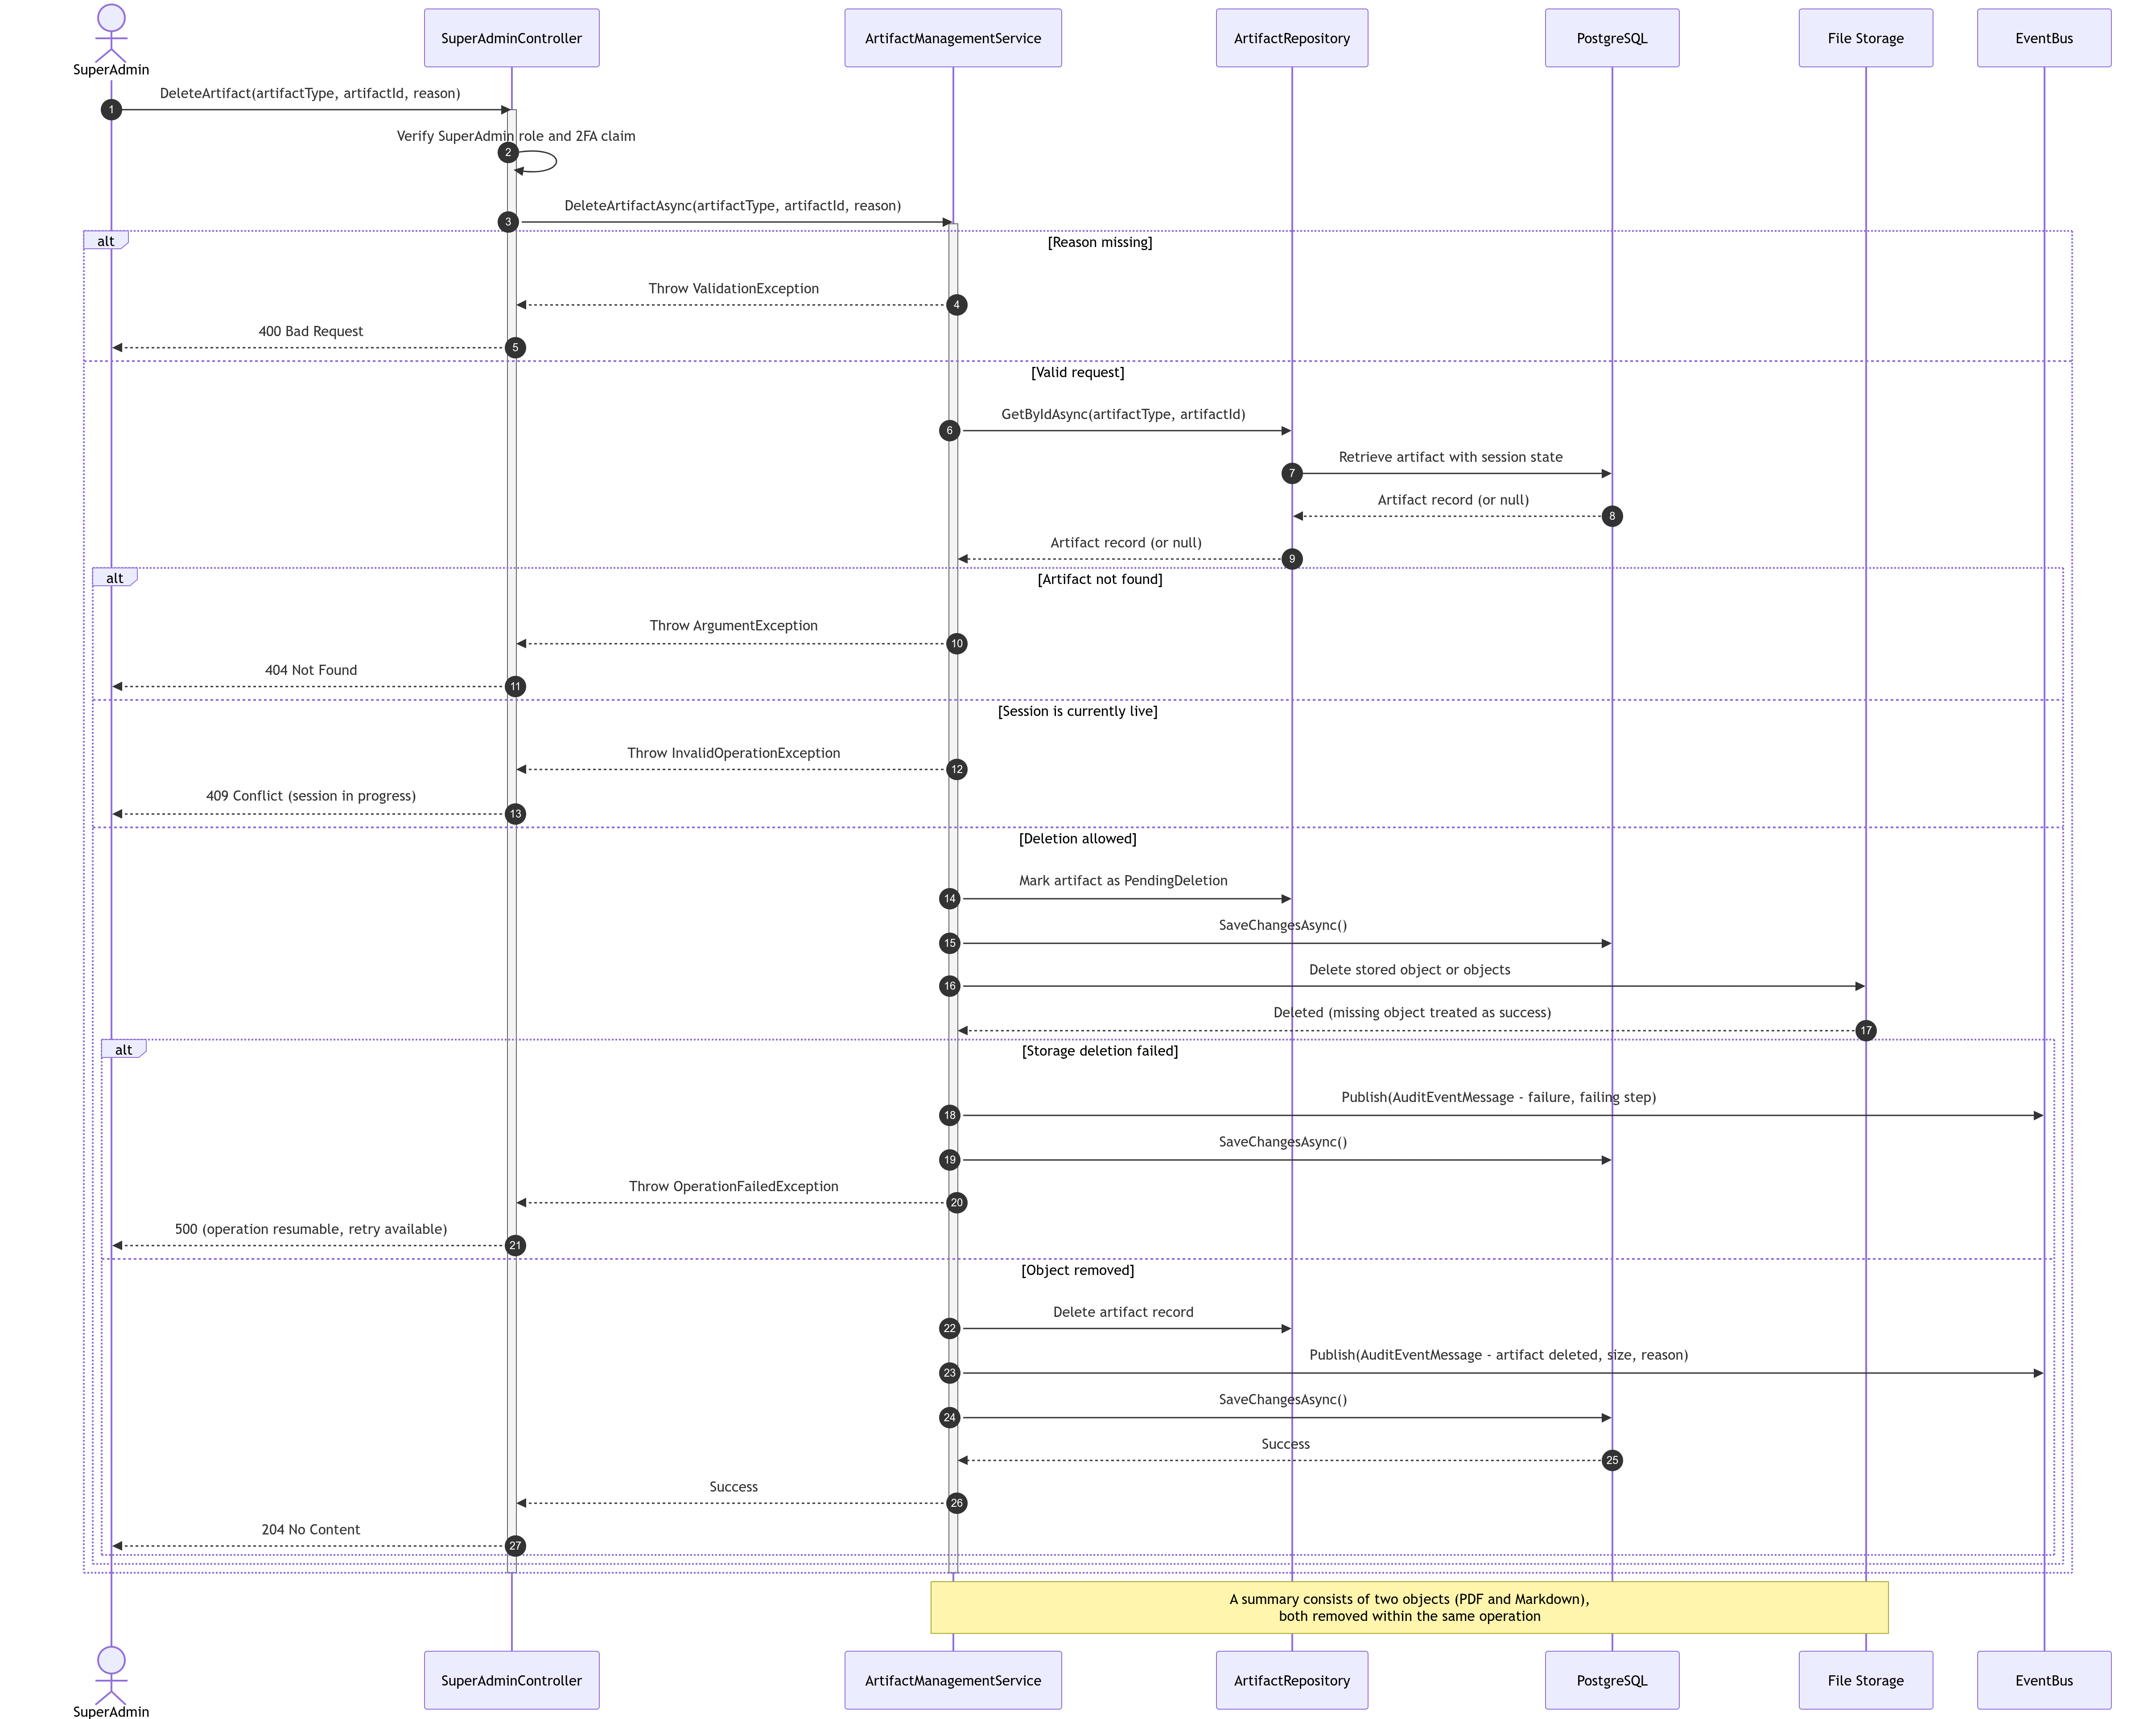
\includegraphics[width=\textwidth,height=0.8\textheight,keepaspectratio]{figures/image43.png}
  \caption{مخطط تسلسل النظام لحالة «حذف تسجيل أو ملخص»: يوضّح الرسائل المتبادلة بين الفاعل والنظام بوصفه صندوقًا أسود، أي دون إظهار الخدمات الداخلية التي تنفّذها.}
  \label{fig:image43}
\end{figure}

\subsubsection{مخطط تسلسل النظام لحالات استخدام الطالب}

\subsection{مخطط تسلسل النظام لحالات استخدام النظام}

\subsubsection{مخطط تسلسل النظام لحالة فهرسة ملفات الفصل}

\begin{figure}[htbp]
  \centering
  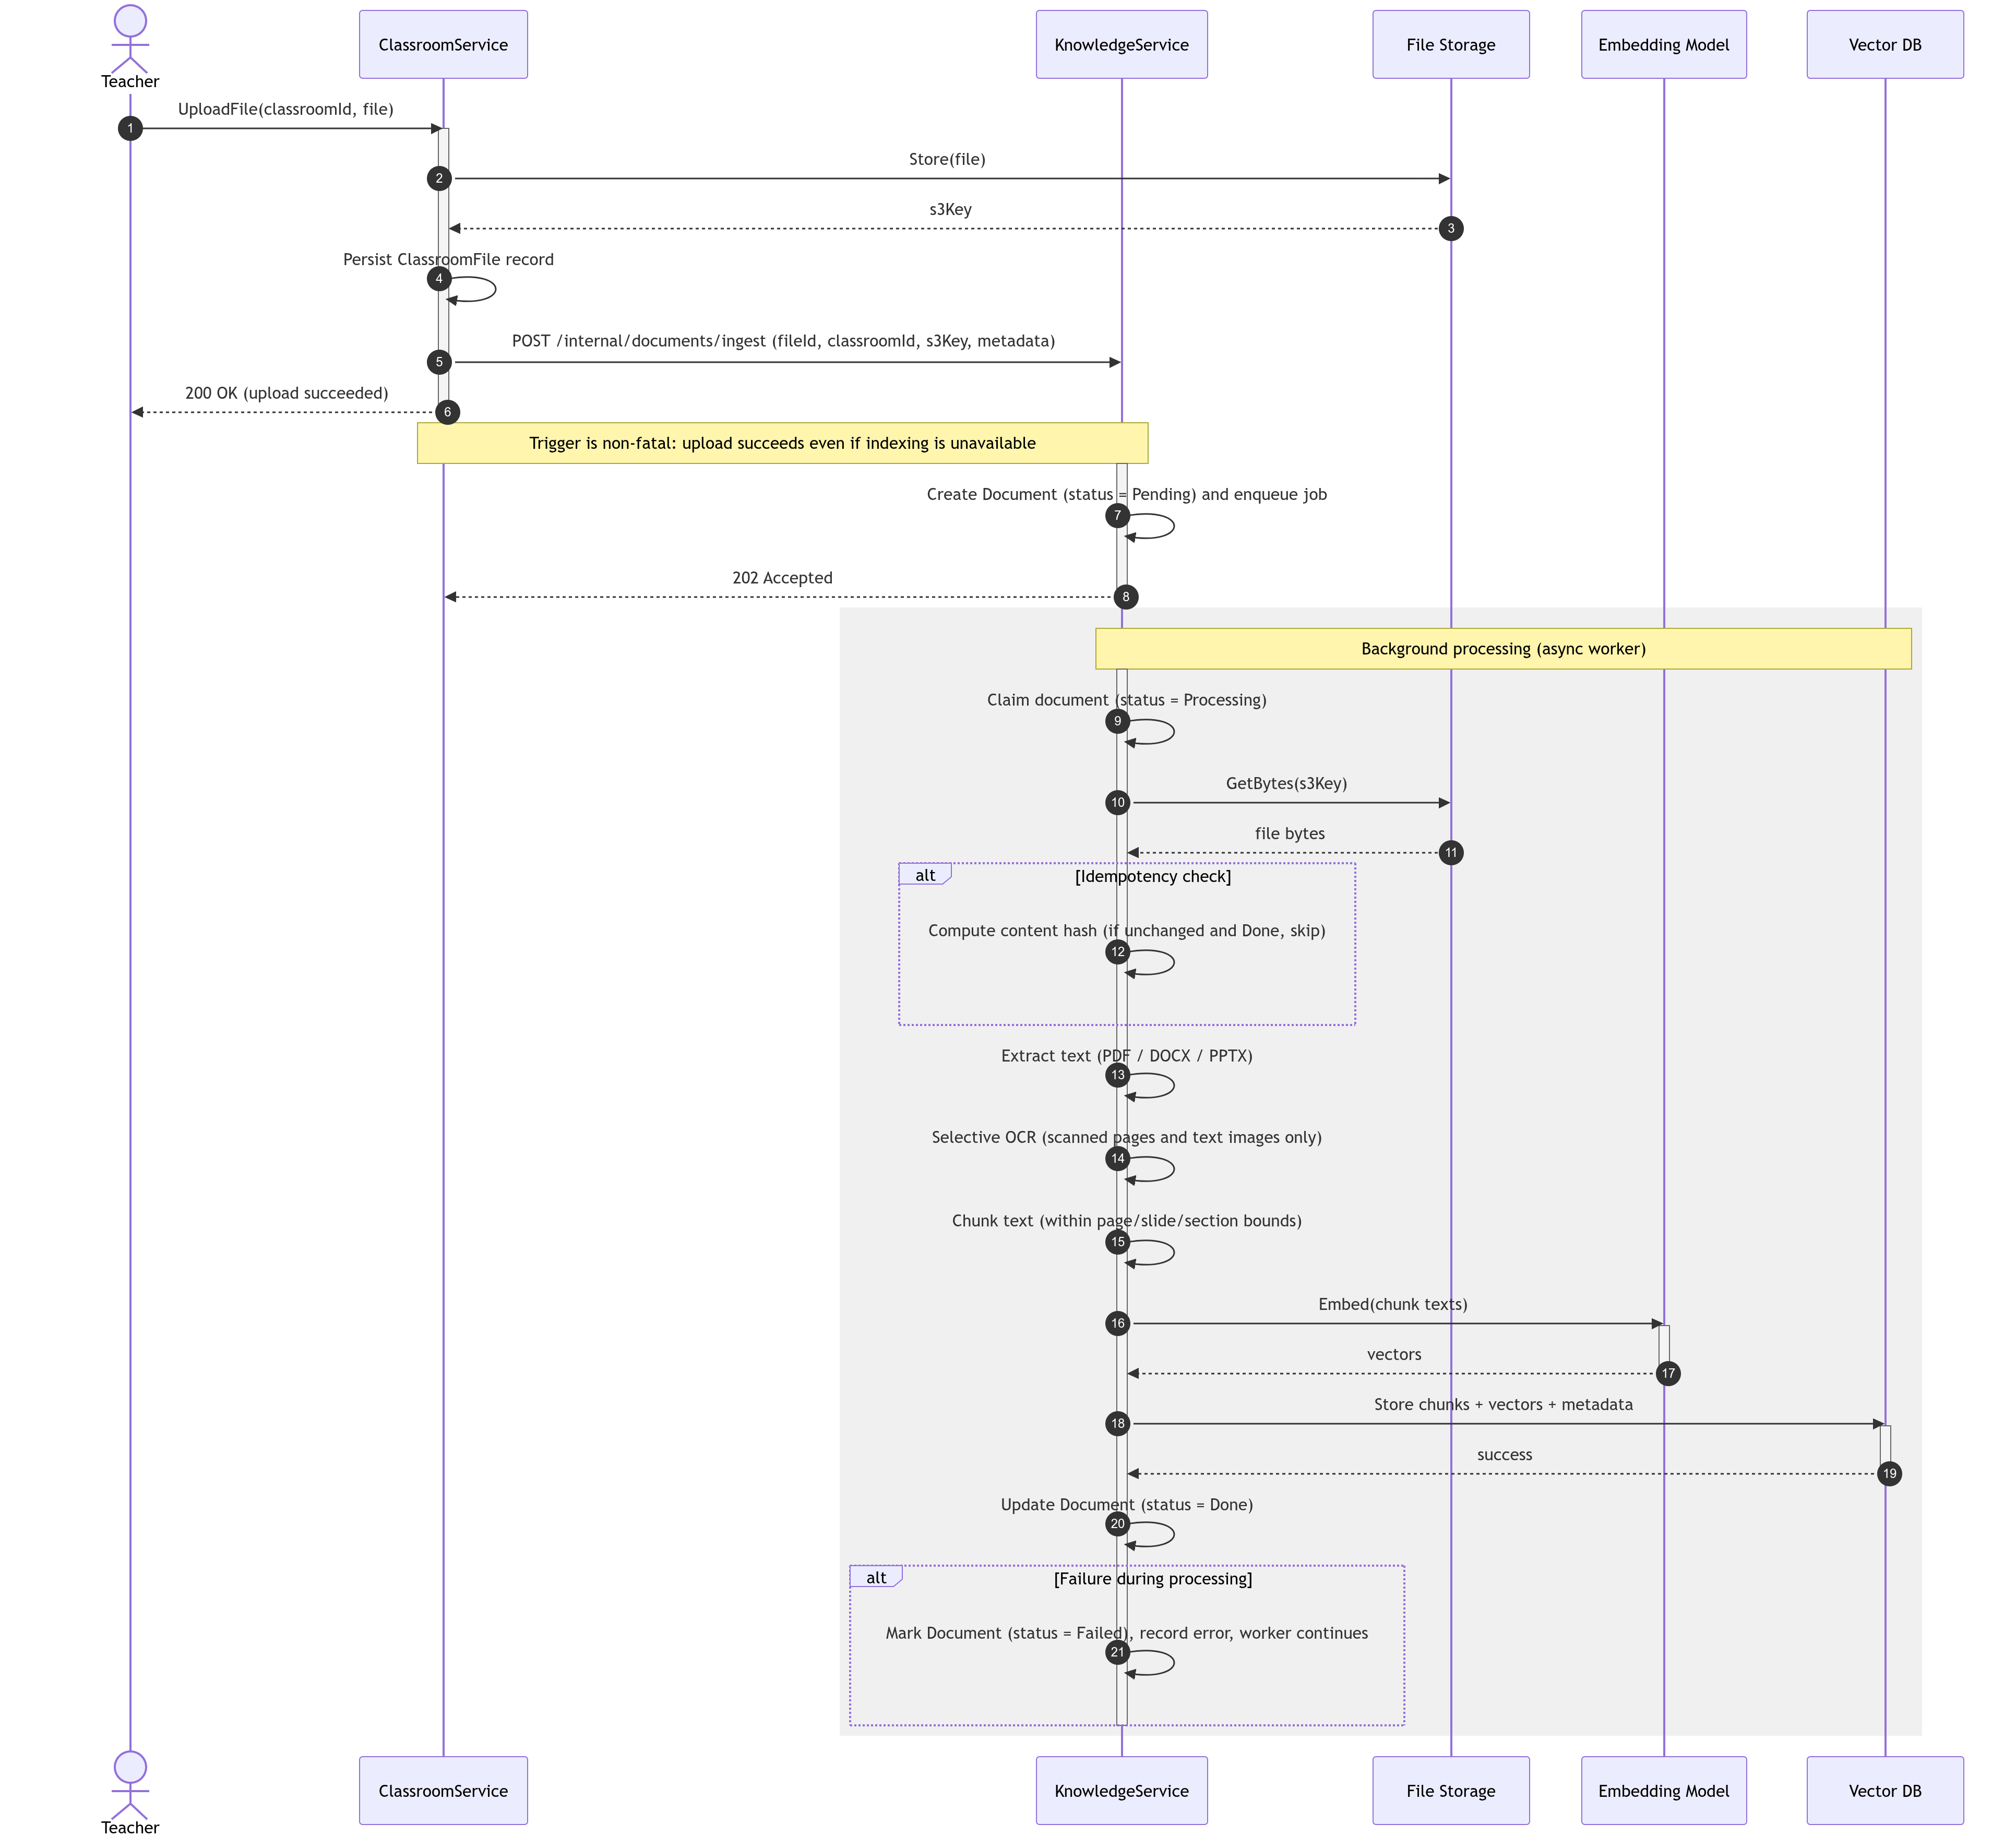
\includegraphics[width=\textwidth,height=0.8\textheight,keepaspectratio]{figures/image48.png}
  \caption{مخطط تسلسل النظام لحالة «فهرسة ملفات الفصل»: يوضّح الرسائل المتبادلة بين الفاعل والنظام بوصفه صندوقًا أسود، أي دون إظهار الخدمات الداخلية التي تنفّذها.}
  \label{fig:image48}
\end{figure}

\subsubsection{مخطط تسلسل النظام لحالة تحليل شرح المعلم مقابل المادة المرجعية}

\begin{figure}[htbp]
  \centering
  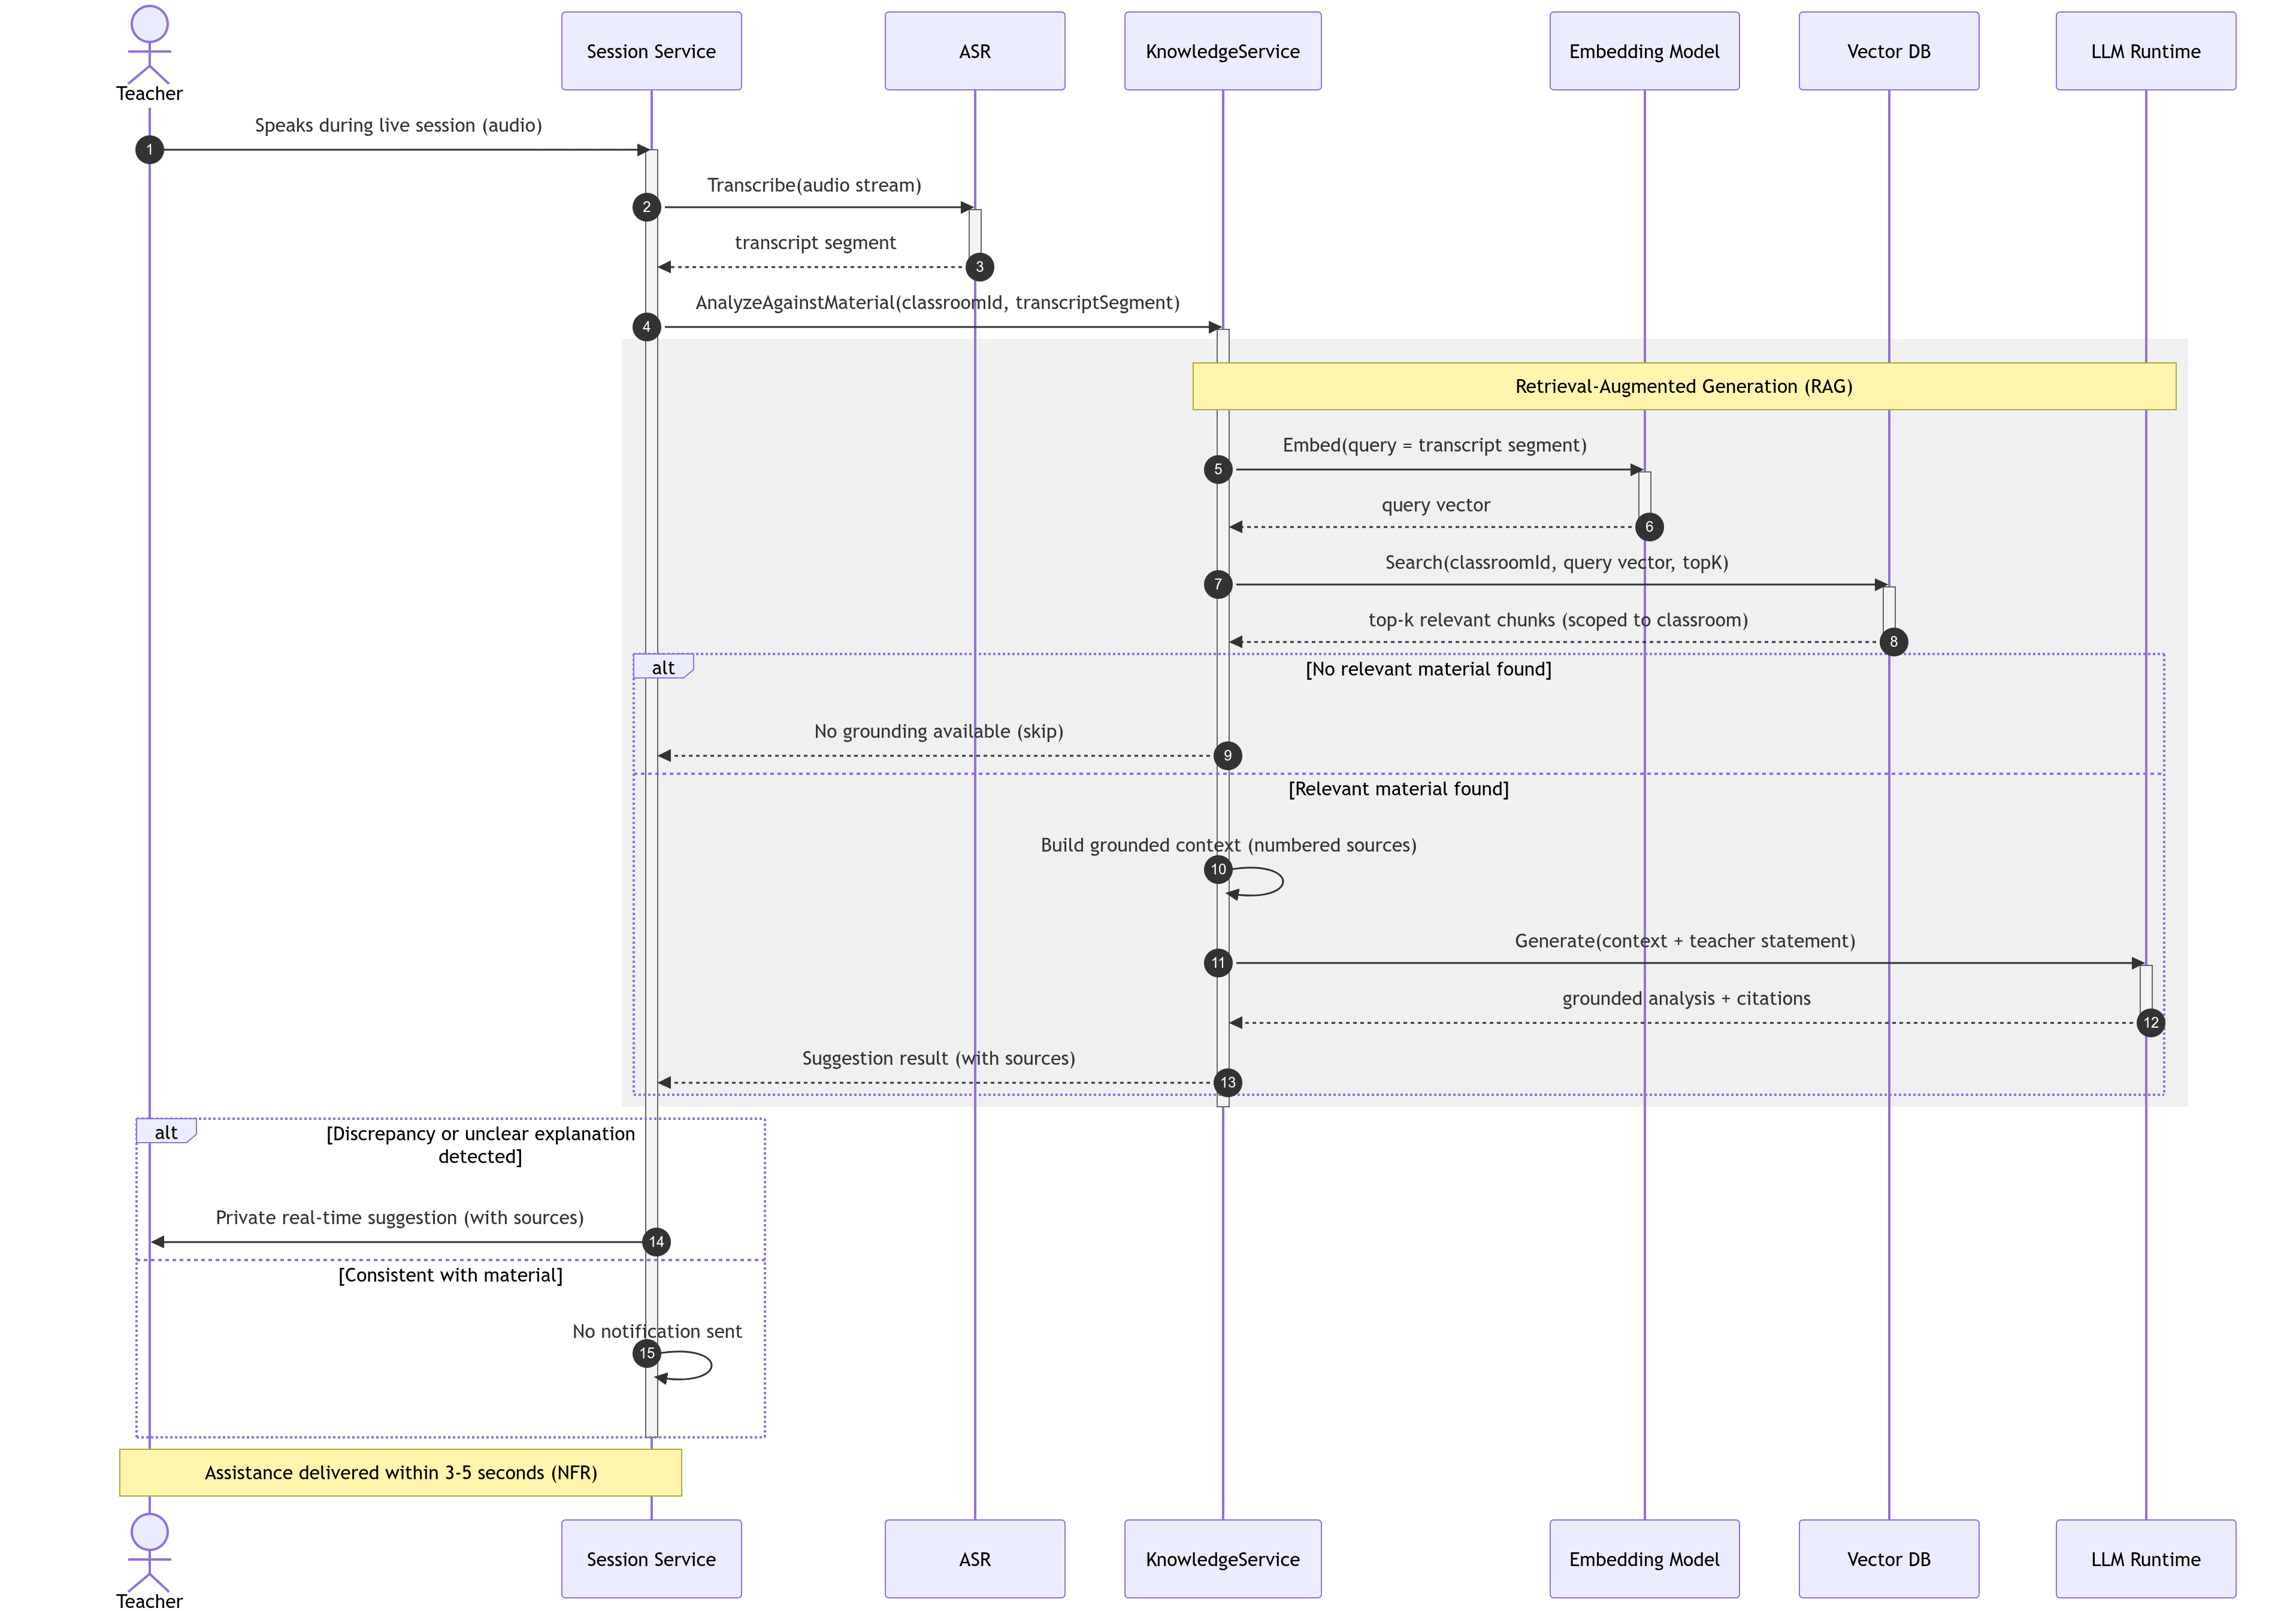
\includegraphics[width=\textwidth,height=0.8\textheight,keepaspectratio]{figures/image49.png}
  \caption{مخطط تسلسل النظام لحالة «تحليل شرح المعلم مقابل المادة المرجعية»: يوضّح الرسائل المتبادلة بين الفاعل والنظام بوصفه صندوقًا أسود، أي دون إظهار الخدمات الداخلية التي تنفّذها.}
  \label{fig:image49}
\end{figure}

\subsubsection{تدفّق الحلقة الحيّة}
\label{subsubsec:flow-live-loop}

يعرض الشكل~\ref{fig:arch-03} الحلقة التي تعمل طوال الجلسة: التقاط الصوت، وتحويله إلى نص، وكشف اكتمال الفكرة، وتقييمها مقابل المصادر المفهرسة، ثمّ اتّخاذ قرار التدخّل من عدمه.

\begin{figure}[htbp]
  \centering
  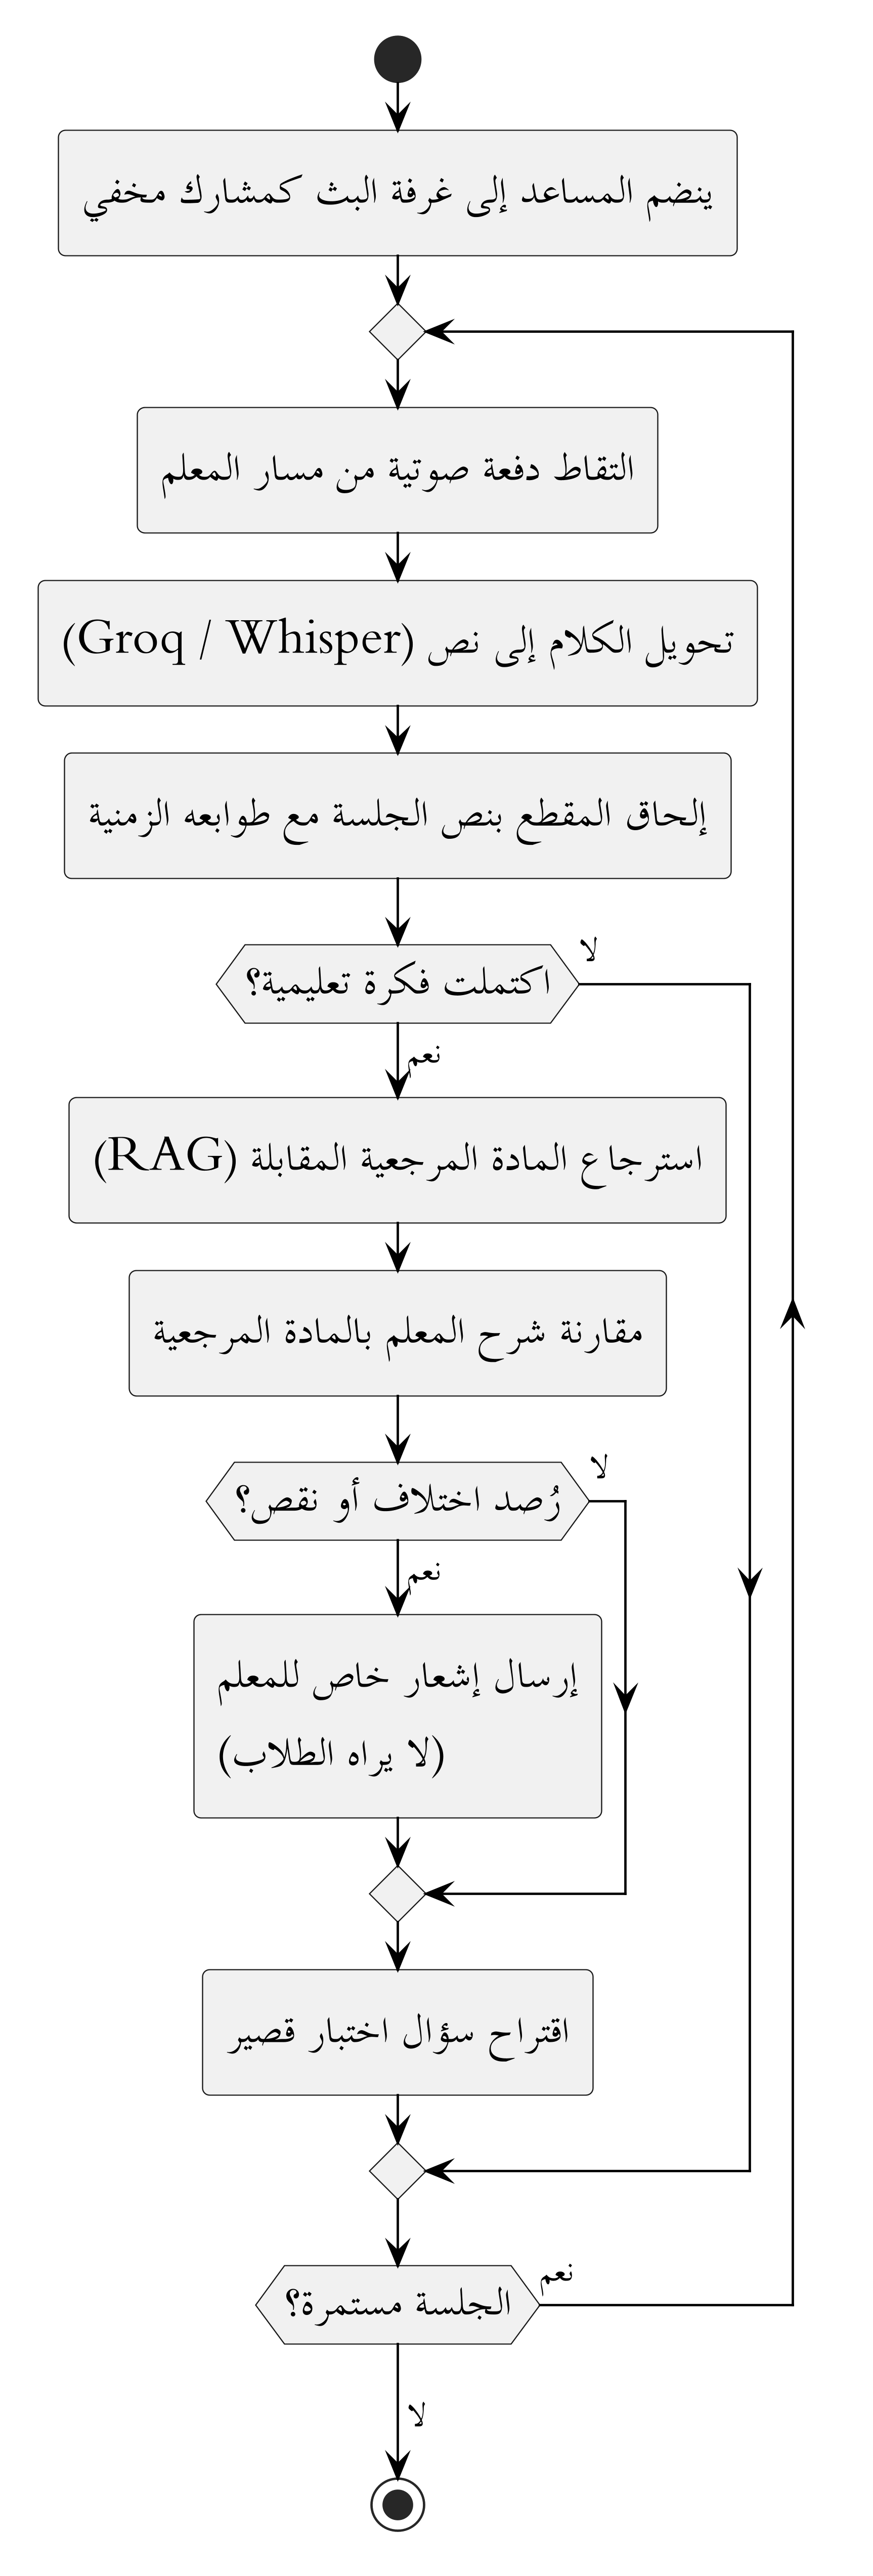
\includegraphics[width=\textwidth,height=0.8\textheight,keepaspectratio]{figures/arch-03-live-assistant.png}
  \caption{تدفّق الحلقة الحيّة في خدمة المساعد المباشر.}
  \label{fig:arch-03}
\end{figure}

\subsubsection{تدفّق تسجيل الجلسة وحفظها}
\label{subsubsec:flow-recording}

يبيّن الشكل~\ref{fig:flow-03} تدفّق تسجيل الجلسة وما اعتُمد فيه من حجزٍ ومُصالِحٍ دوريّ لمعالجة التبعية لنظام خارجي.

\begin{figure}[htbp]
  \centering
  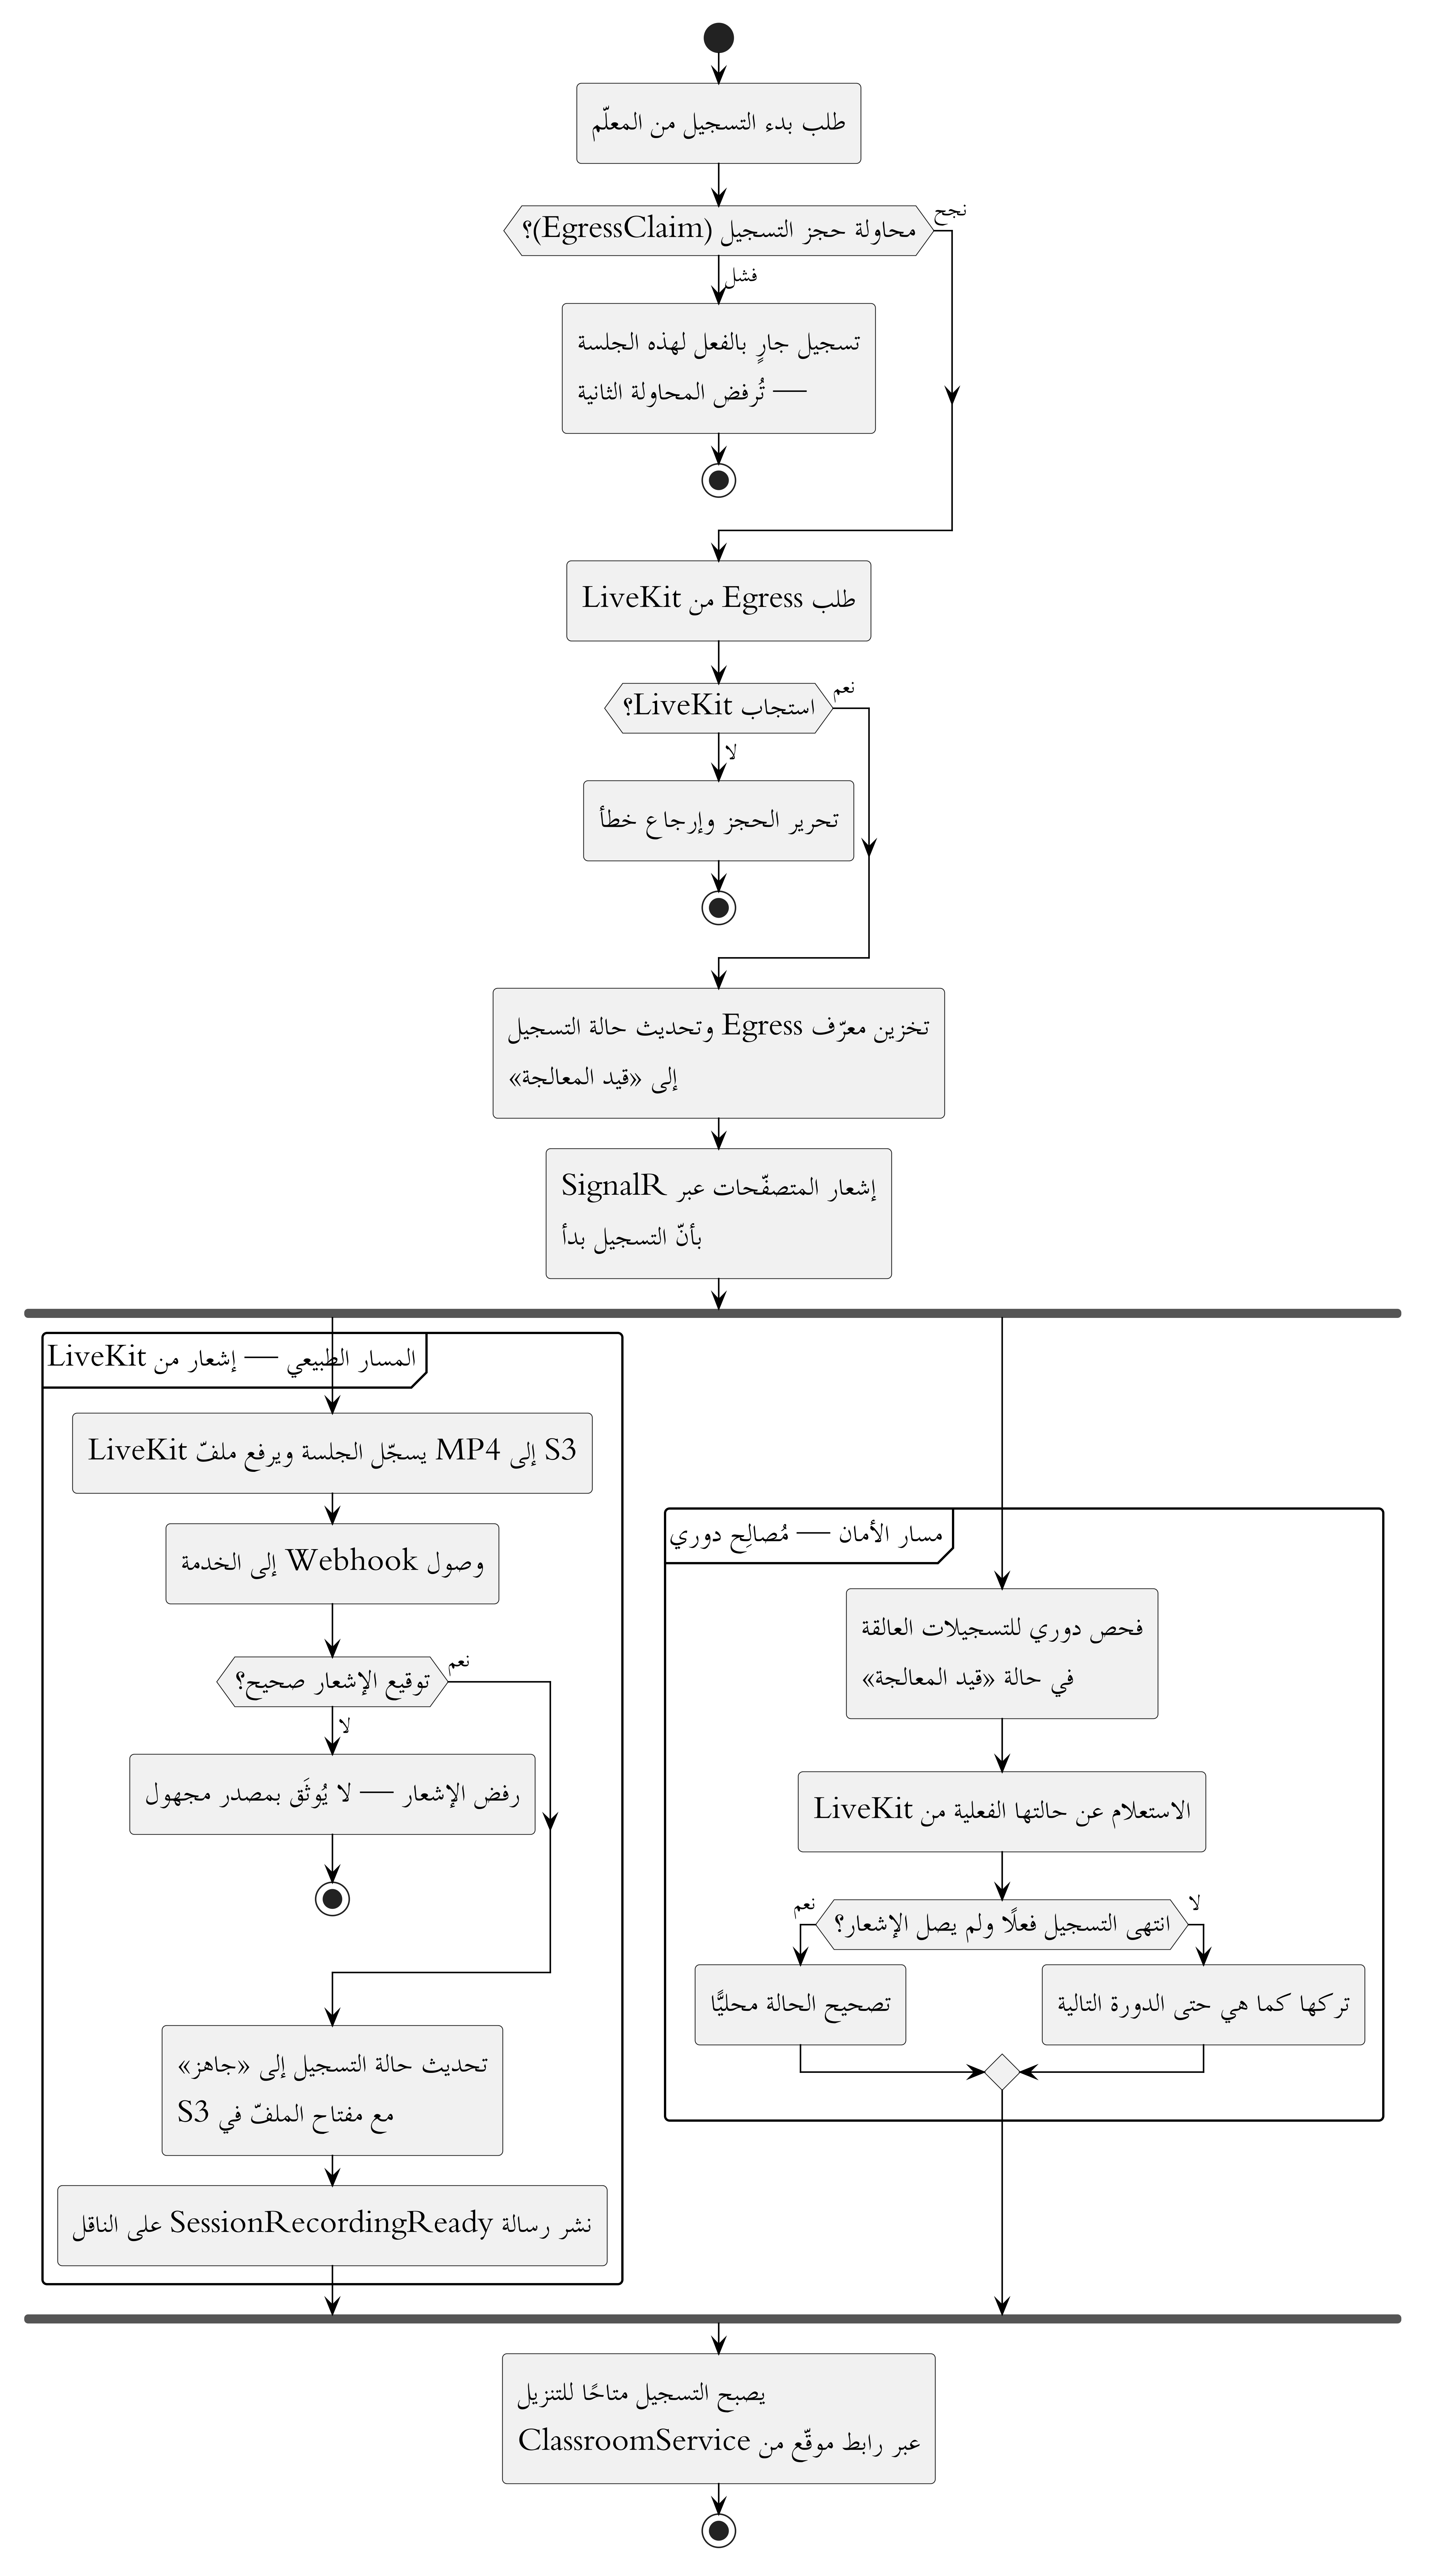
\includegraphics[width=\textwidth,height=0.8\textheight,keepaspectratio]{figures/flow-03-recording-egress.png}
  \caption{تدفّق تسجيل الجلسة وحفظها في مخزن الملفّات.}
  \label{fig:flow-03}
\end{figure}

\noindent يعتمد تدفّق التسجيل على نظام خارجي، ولا تستطيع خدمة البث إتمامه وحدها. وقد بُيّنت معالجة هذه التبعية في الشكل~\ref{fig:flow-03}.

واعتُمدت آليتان متكاملتان لمعالجة هذه التبعية:

\begin{enumerate}
  \item \textbf{الحجز} (\en{EgressClaim}): يمنع بدء تسجيلين متوازيين للجلسة نفسها، وهو احتمال قائم عند الضغط على زرّ التسجيل مرّتين قبل وصول جواب \en{LiveKit} عن الطلب الأول.
  \item \textbf{المُصالِح الدوري} (\en{Reconciler}): يفحص دوريًّا التسجيلات العالقة في حالة المعالجة، ويستعلم عن حالتها الفعلية من \en{LiveKit}، ويصحّحها محلّيًّا. ويحافظ ذلك على صحّة الحالة حتى عند فقد الإشعار.
\end{enumerate}

\subsubsection{تدفّق إرسال الإشعارات البريدية}
\label{subsubsec:flow-email}

\begin{figure}[htbp]
  \centering
  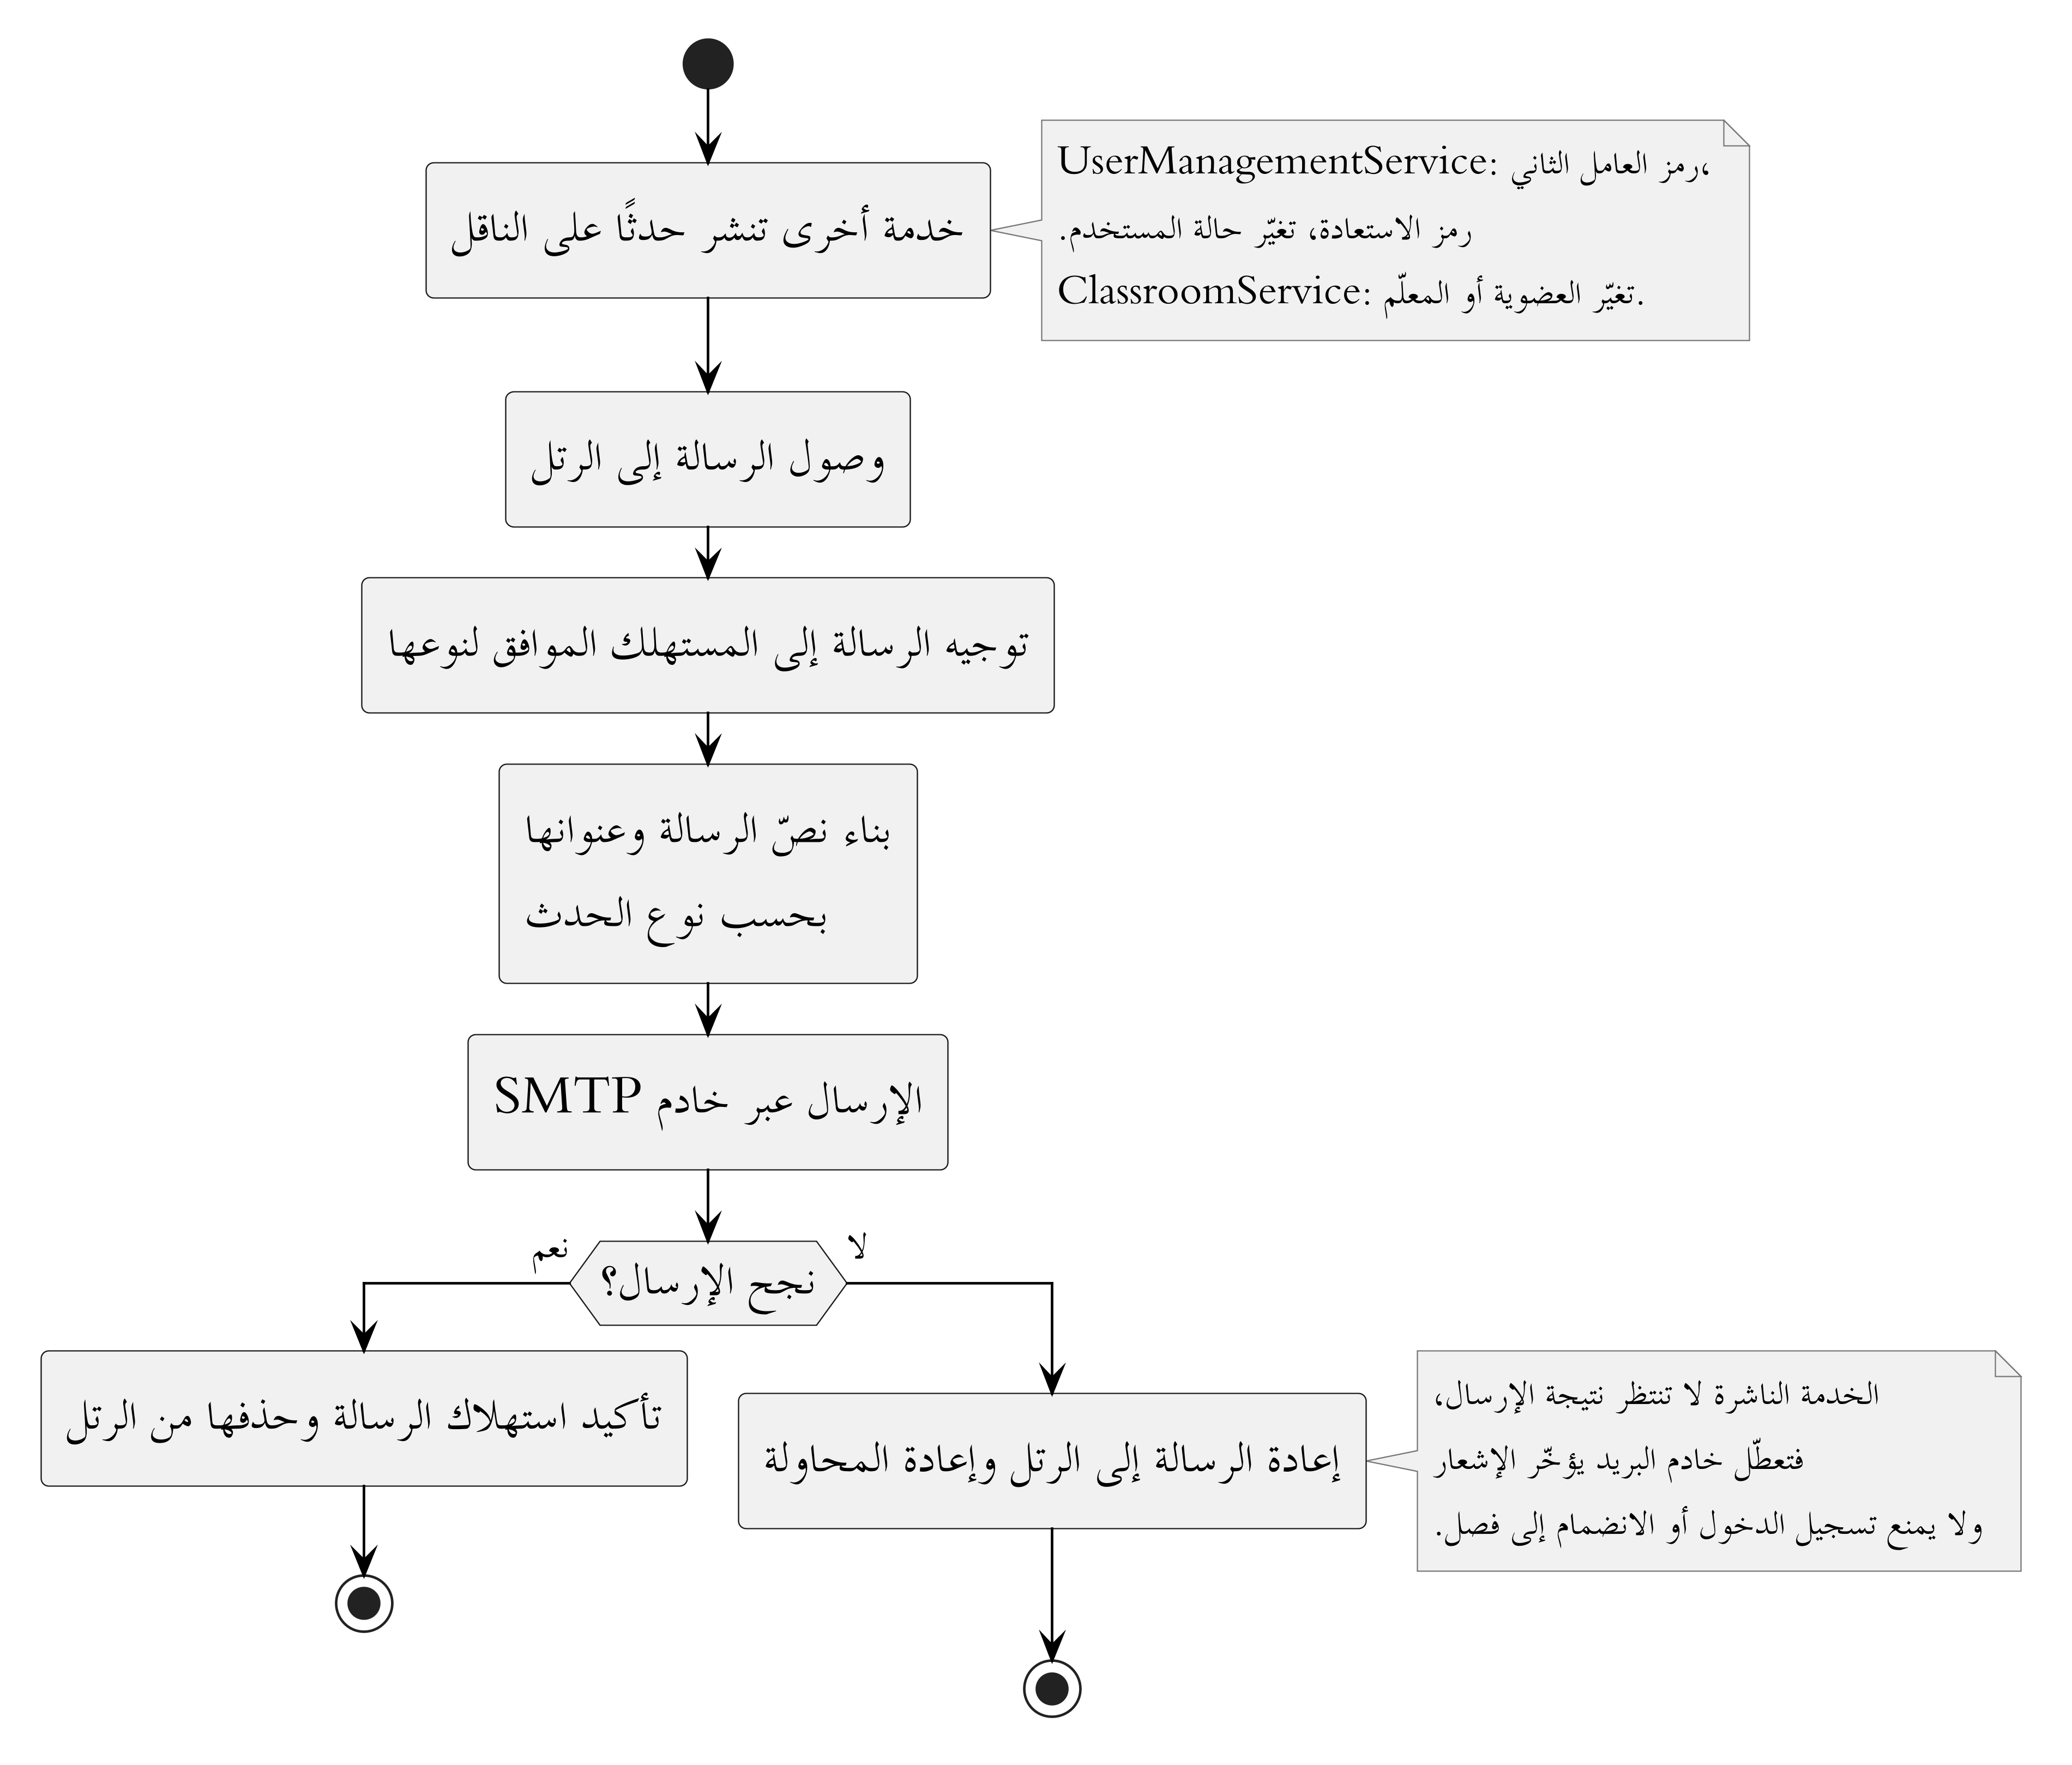
\includegraphics[width=\textwidth,height=0.8\textheight,keepaspectratio]{figures/flow-04-email-dispatch.png}
  \caption{تدفّق إرسال الإشعارات البريدية.}
  \label{fig:flow-04}
\end{figure}

\noindent وقد بُيّن مسار الإشعار من لحظة نشره إلى لحظة تسليمه في الشكل~\ref{fig:flow-04}.

ويحقّق عزل هذه المسؤولية في خدمة مستهلِكة فكَّ الارتباط الزمني، إذ لا تنتظر الخدمة الناشرة نتيجة الإرسال. ويؤدّي تعطّل خادم البريد عندئذٍ إلى تأخير وصول الإشعارات دون تعطيل تسجيل الدخول أو التسجيل أو الانضمام إلى فصل.

\subsubsection{تدفّق استيعاب المستندات وفهرستها}
\label{subsubsec:flow-ingestion}

يبيّن الشكل~\ref{fig:arch-02} مراحل خط أنابيب الاستيعاب، وتُعالَج جميعها بشكل غير متزامن في الخلفية تفادياً لتعطيل رفع الملفّ بانتظار المعالجة الثقيلة.

\begin{figure}[htbp]
  \centering
  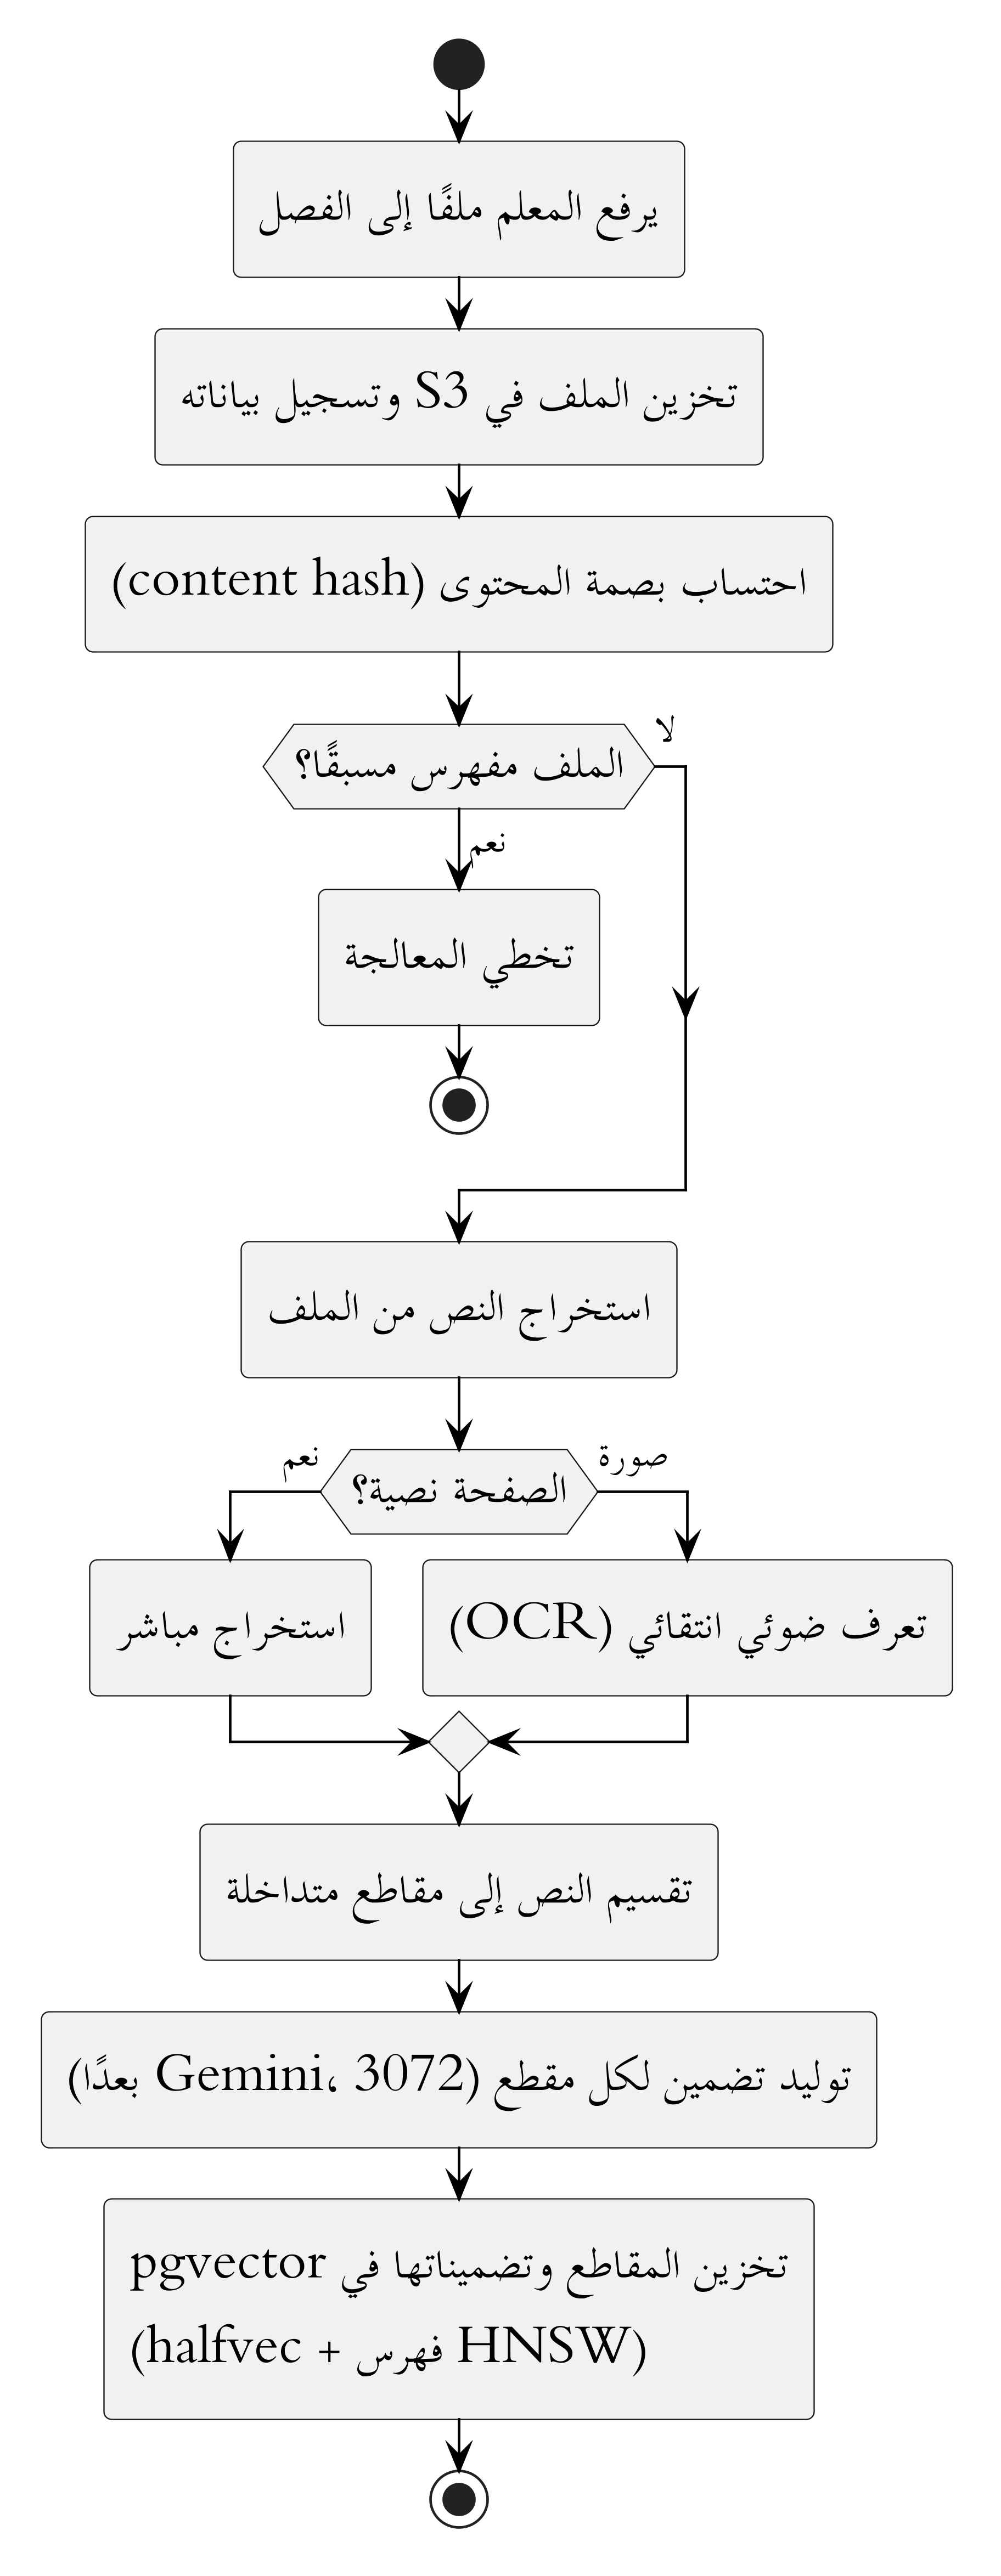
\includegraphics[width=\textwidth,height=0.8\textheight,keepaspectratio]{figures/arch-02-rag-pipeline.png}
  \caption{تدفّق استيعاب المستندات وفهرستها في خدمة الاسترجاع.}
  \label{fig:arch-02}
\end{figure}

% CH2-REF: originally ended "والكلفة (القسم~\ref{subsec:text-extraction-ocr})." — restore with chapter 2.
\noindent واعتُمد عامل معالجة محدود التزامن، ممّا يتيح التحكّم في استهلاك الموارد ويمنع استنزاف الجهاز عند معالجة عدّة ملفّات معاً. وصُمّمت المعالجة خاملة التكرار (\en{Idempotent})، فلا تُعاد فهرسة الملفّ نفسه دون تغيّر في محتواه، مع دعم إعادة الفهرسة عند تغيّره. ويُطبَّق التعرّف الضوئي (\en{OCR}) على الصفحات الممسوحة والصور الحاملة للنص فقط، موازنةً بين الدقة والكلفة.

ويقوم خط الأنابيب على نمط المنافذ والمحوِّلات، فيُحصر استبدال مزوّد التضمين أو محرّك التعرّف الضوئي في محوِّل واحد دون تعديل منطق الخط. ويعرض الشكل~\ref{fig:class-01} هذا التصميم.

\begin{figure}[htbp]
  \centering
  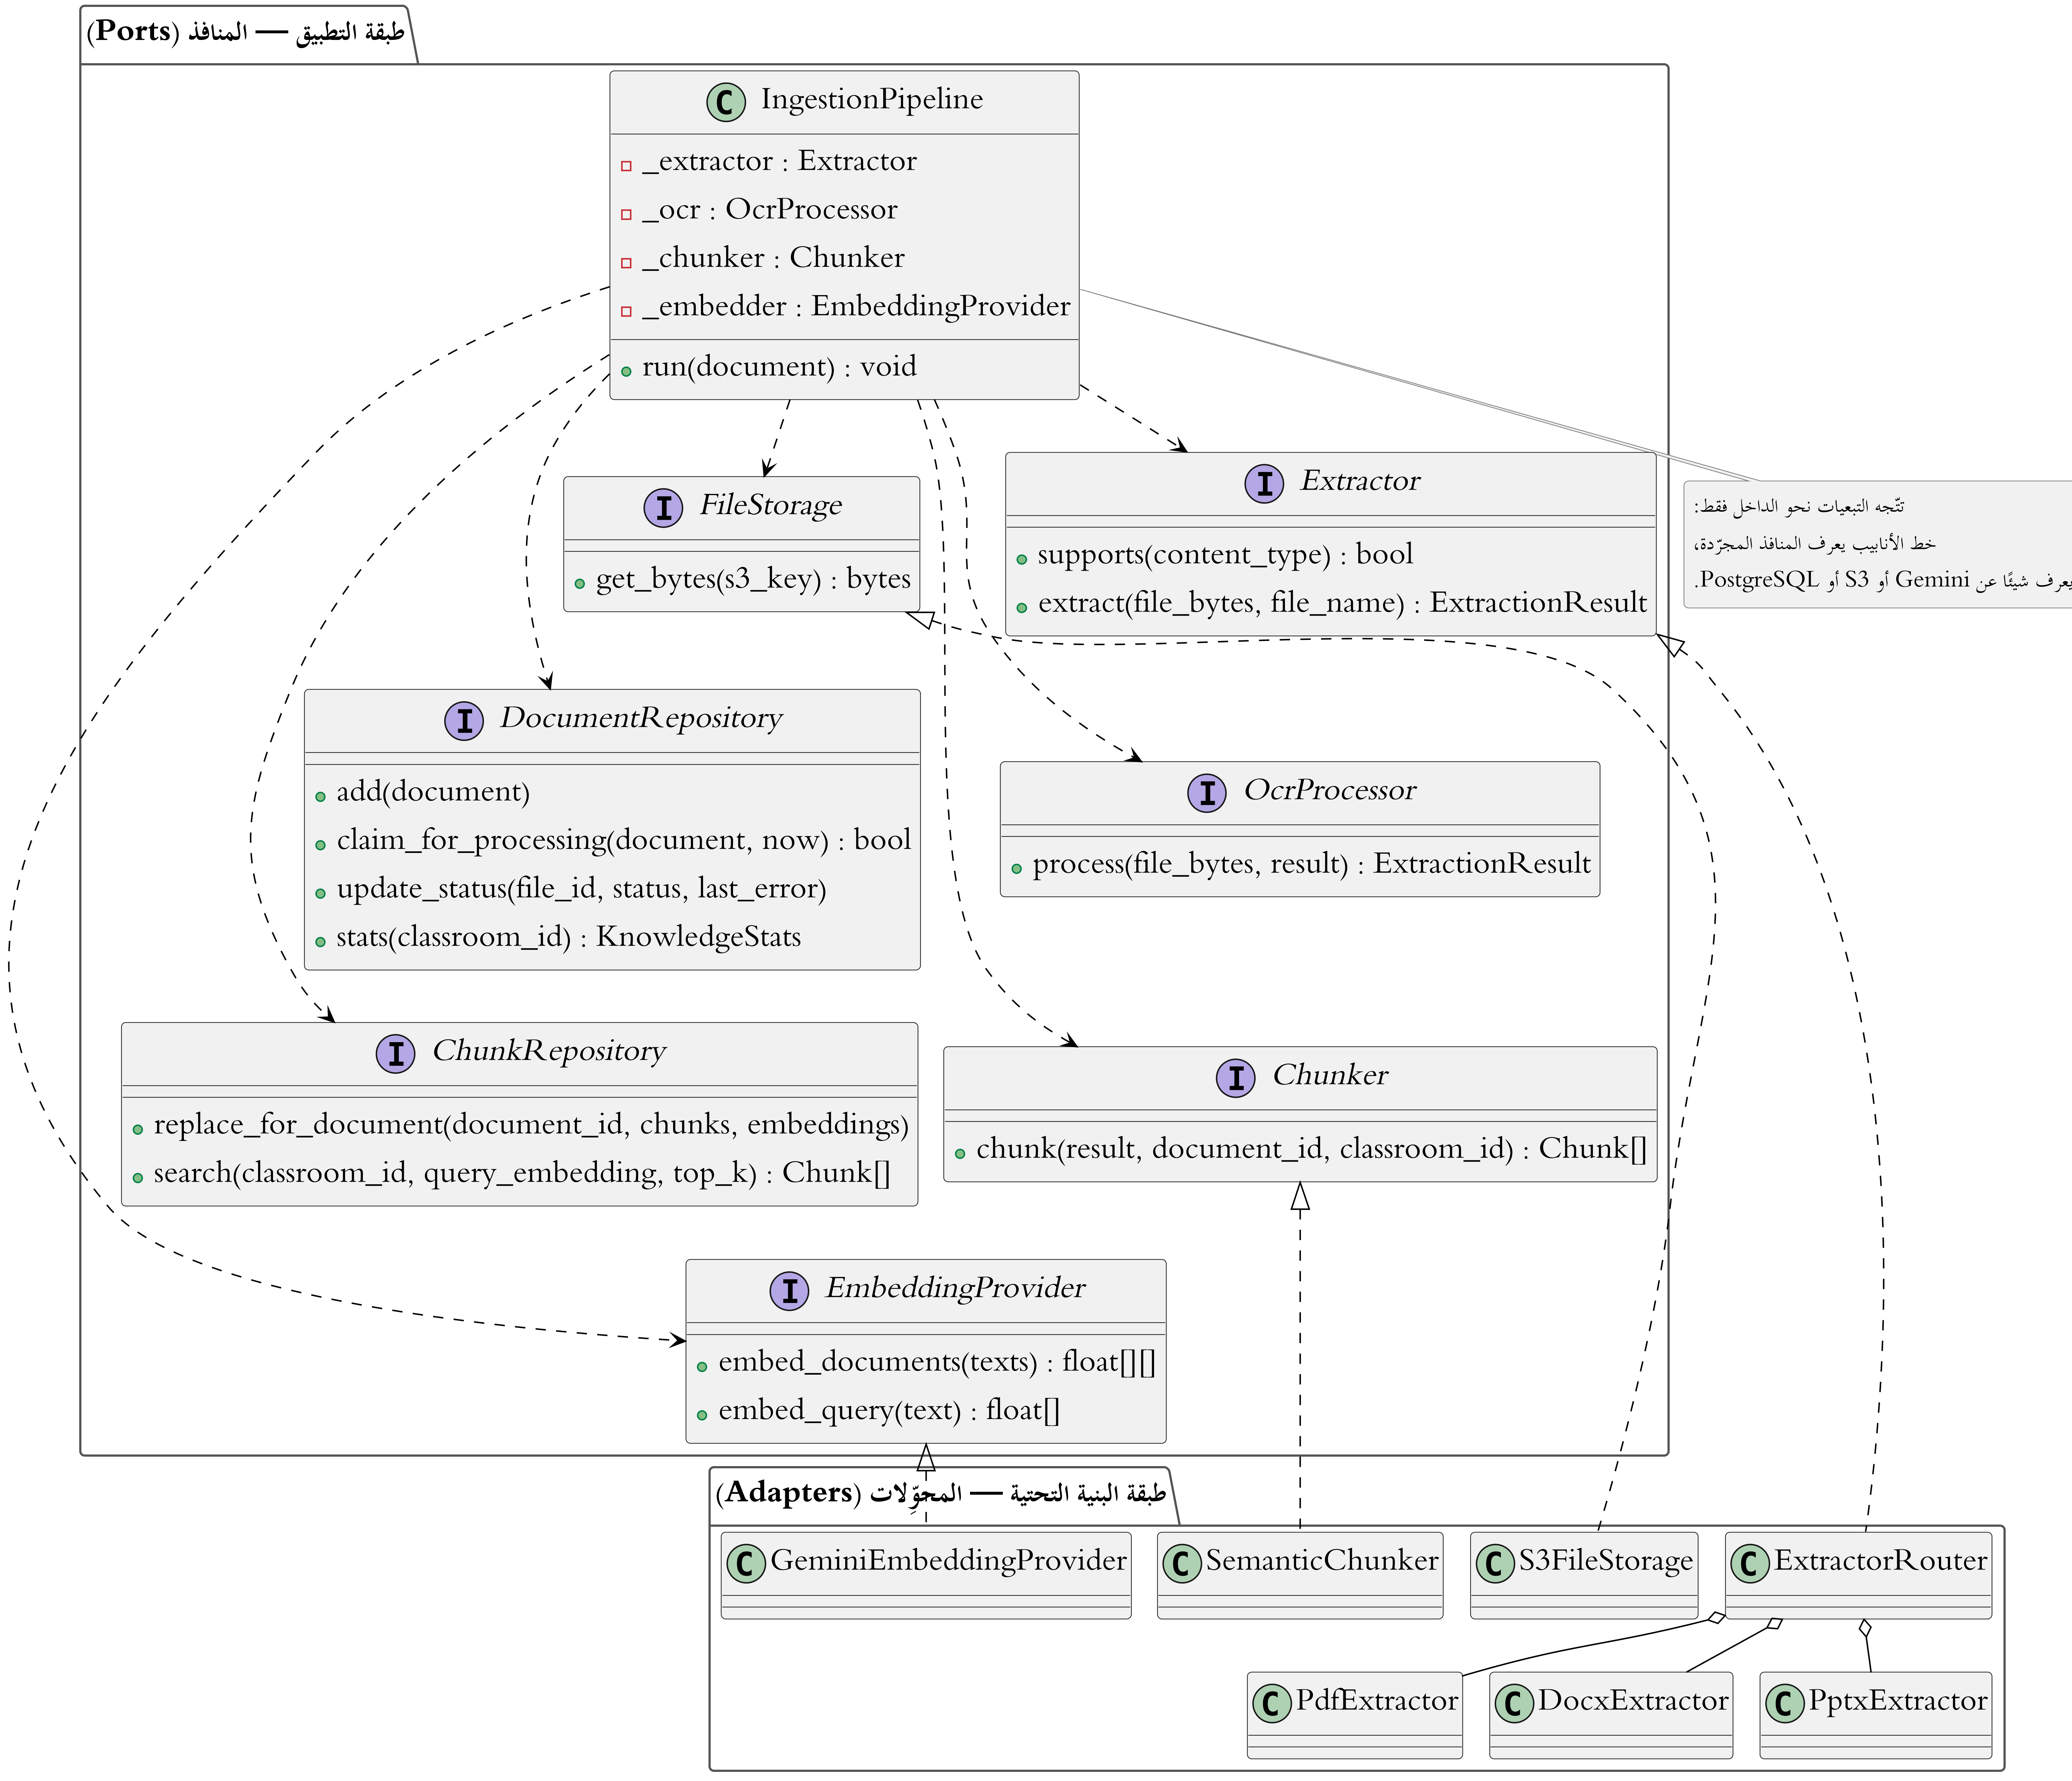
\includegraphics[width=\textwidth,height=0.8\textheight,keepaspectratio]{figures/class-01-ports-adapters.png}
  \caption{مخطط الصفوف لنمط المنافذ والمحوِّلات في خط أنابيب الاستيعاب.}
  \label{fig:class-01}
\end{figure}

\subsubsection{تدفّق الاسترجاع والإجابة}
\label{subsubsec:flow-retrieval}

يبيّن الشكل~\ref{fig:arch-02b} مسار الإجابة عن سؤال: تضمين السؤال، ثمّ البحث الدلالي المقصور على الفصل، ثمّ بناء السياق ضمن حدّ الرموز المتاح، ثمّ توليد الإجابة مؤصَّلةً في المقاطع المسترجَعة.

\begin{figure}[htbp]
  \centering
  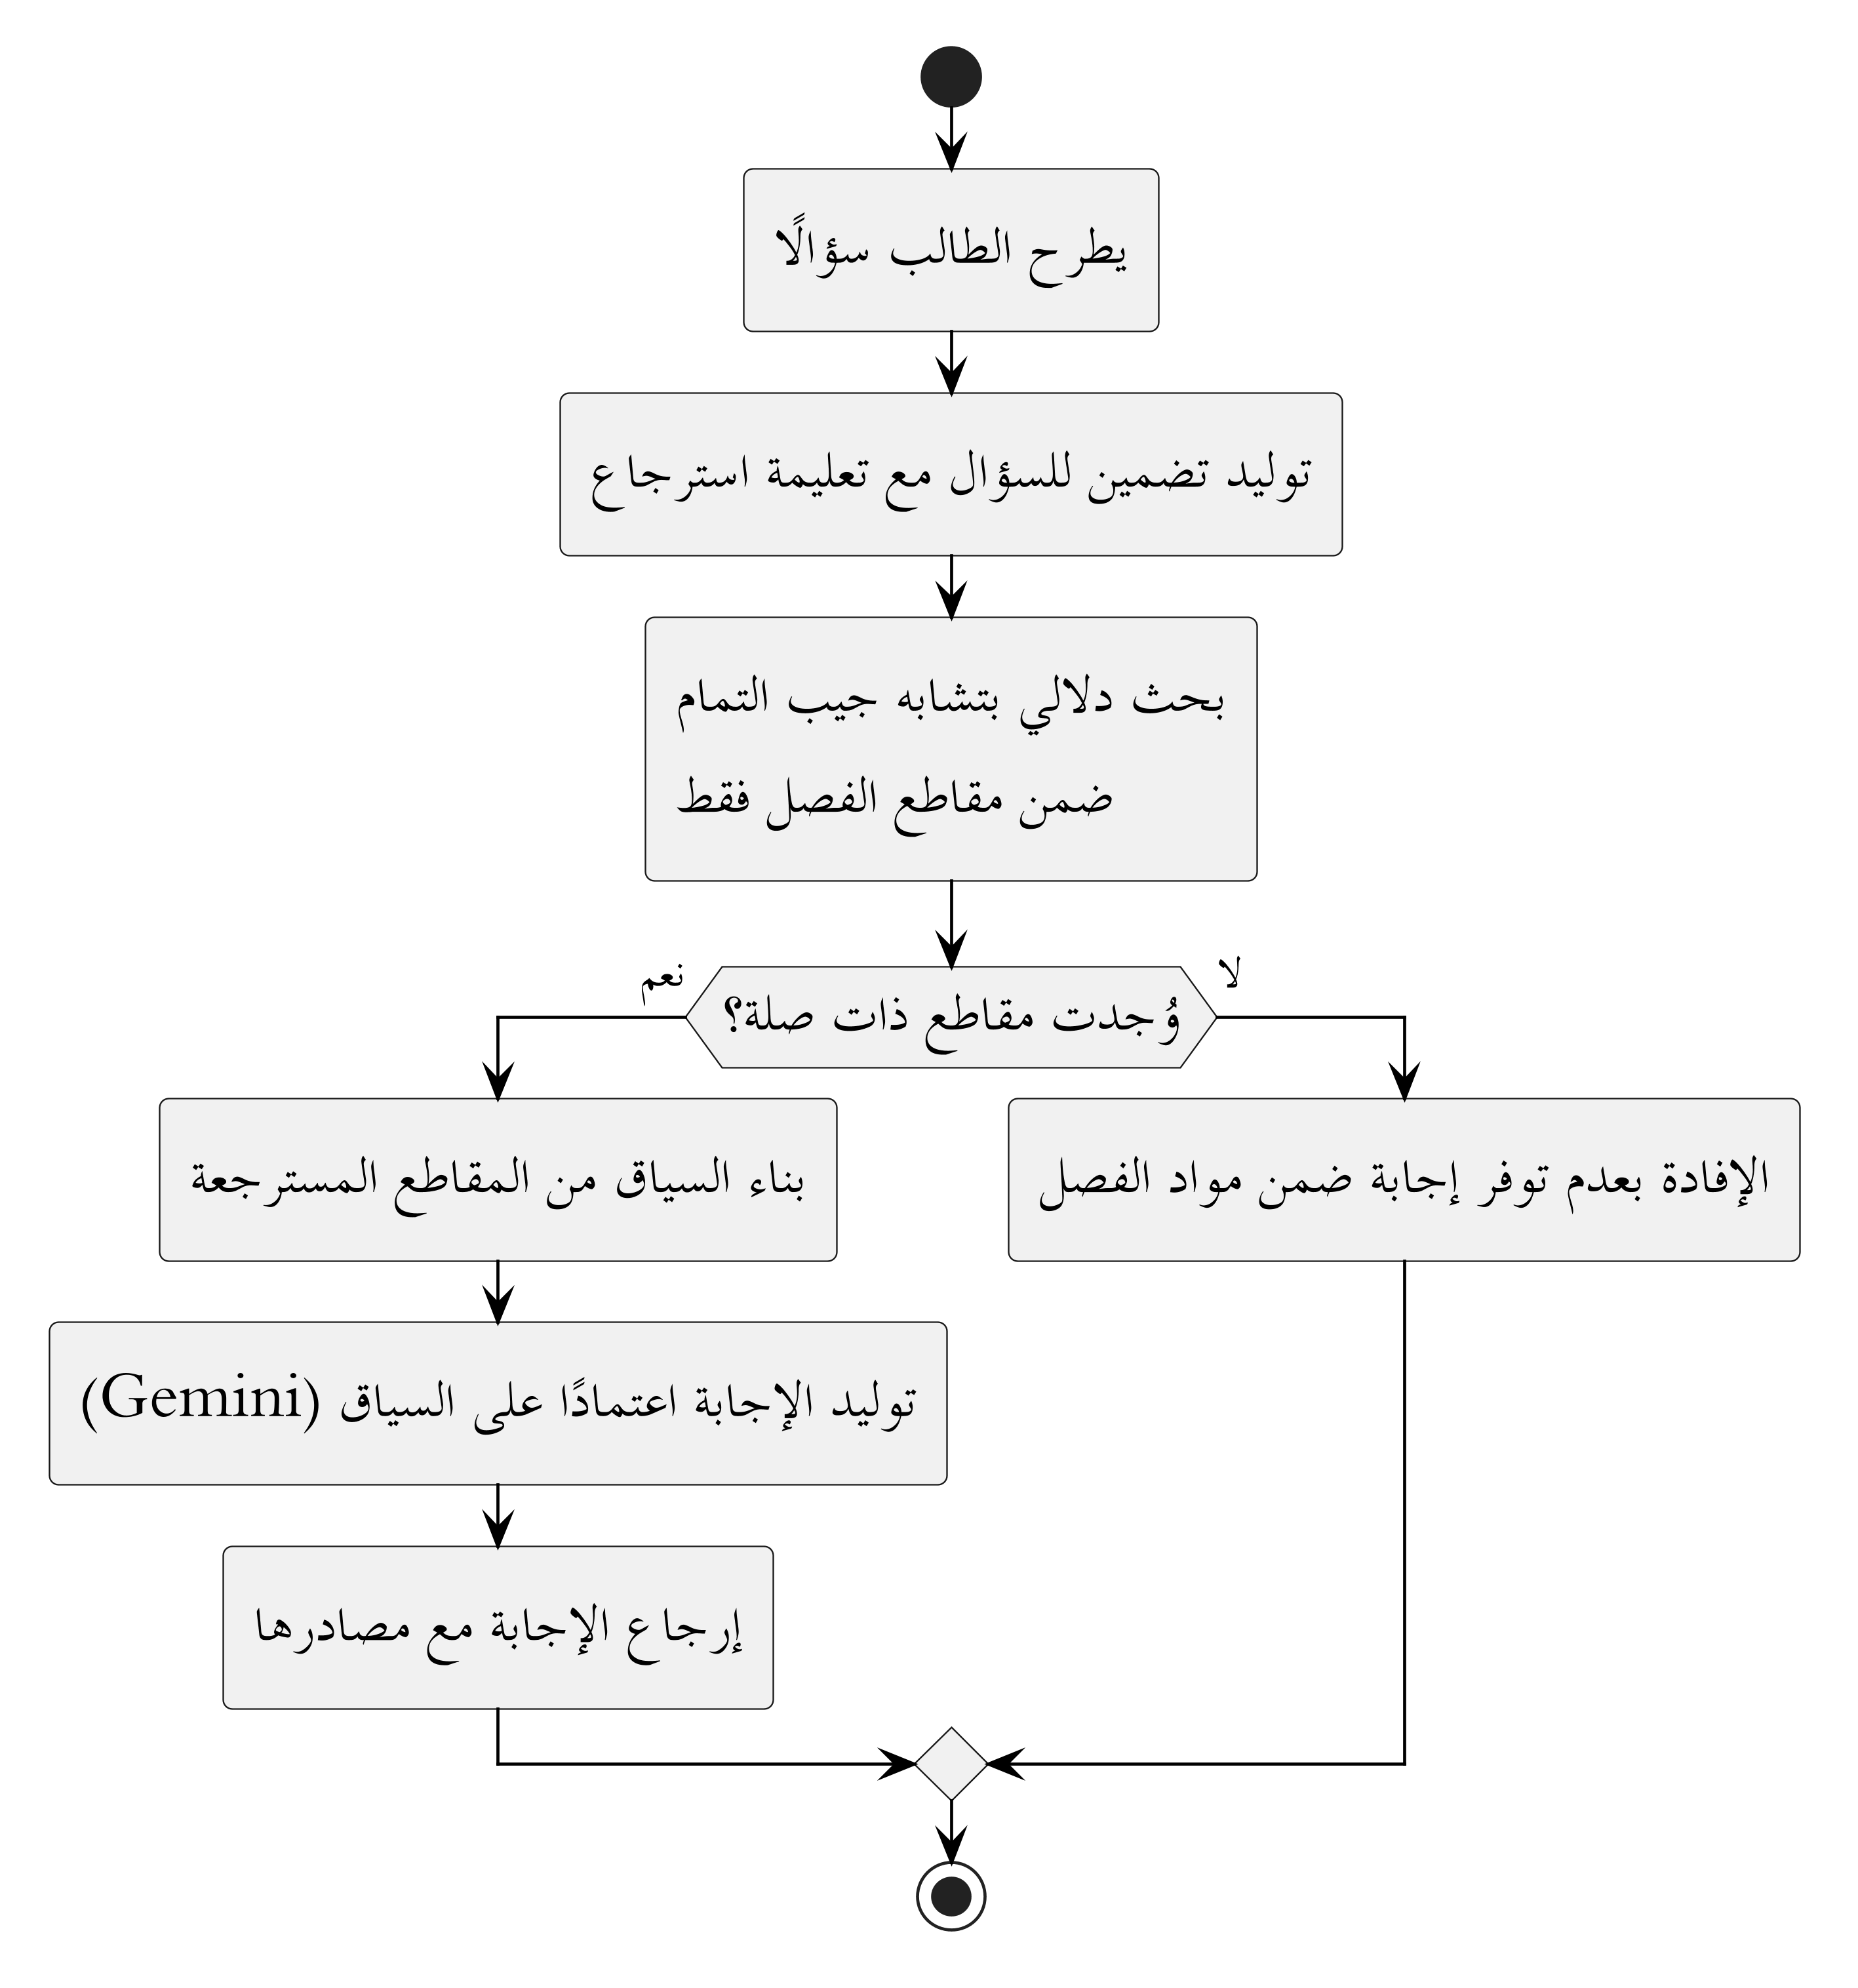
\includegraphics[width=\textwidth,height=0.8\textheight,keepaspectratio]{figures/arch-02b-rag-retrieval.png}
  \caption{تدفّق الاسترجاع وتوليد الإجابة عن سؤال الطالب.}
  \label{fig:arch-02b}
\end{figure}

\subsubsection{تدفّق توليد ملخّص الجلسة}
\label{subsubsec:flow-summary}

يبيّن الشكل~\ref{fig:arch-03b} مسار توليد ملخّص الجلسة بعد انتهائها.

\begin{figure}[htbp]
  \centering
  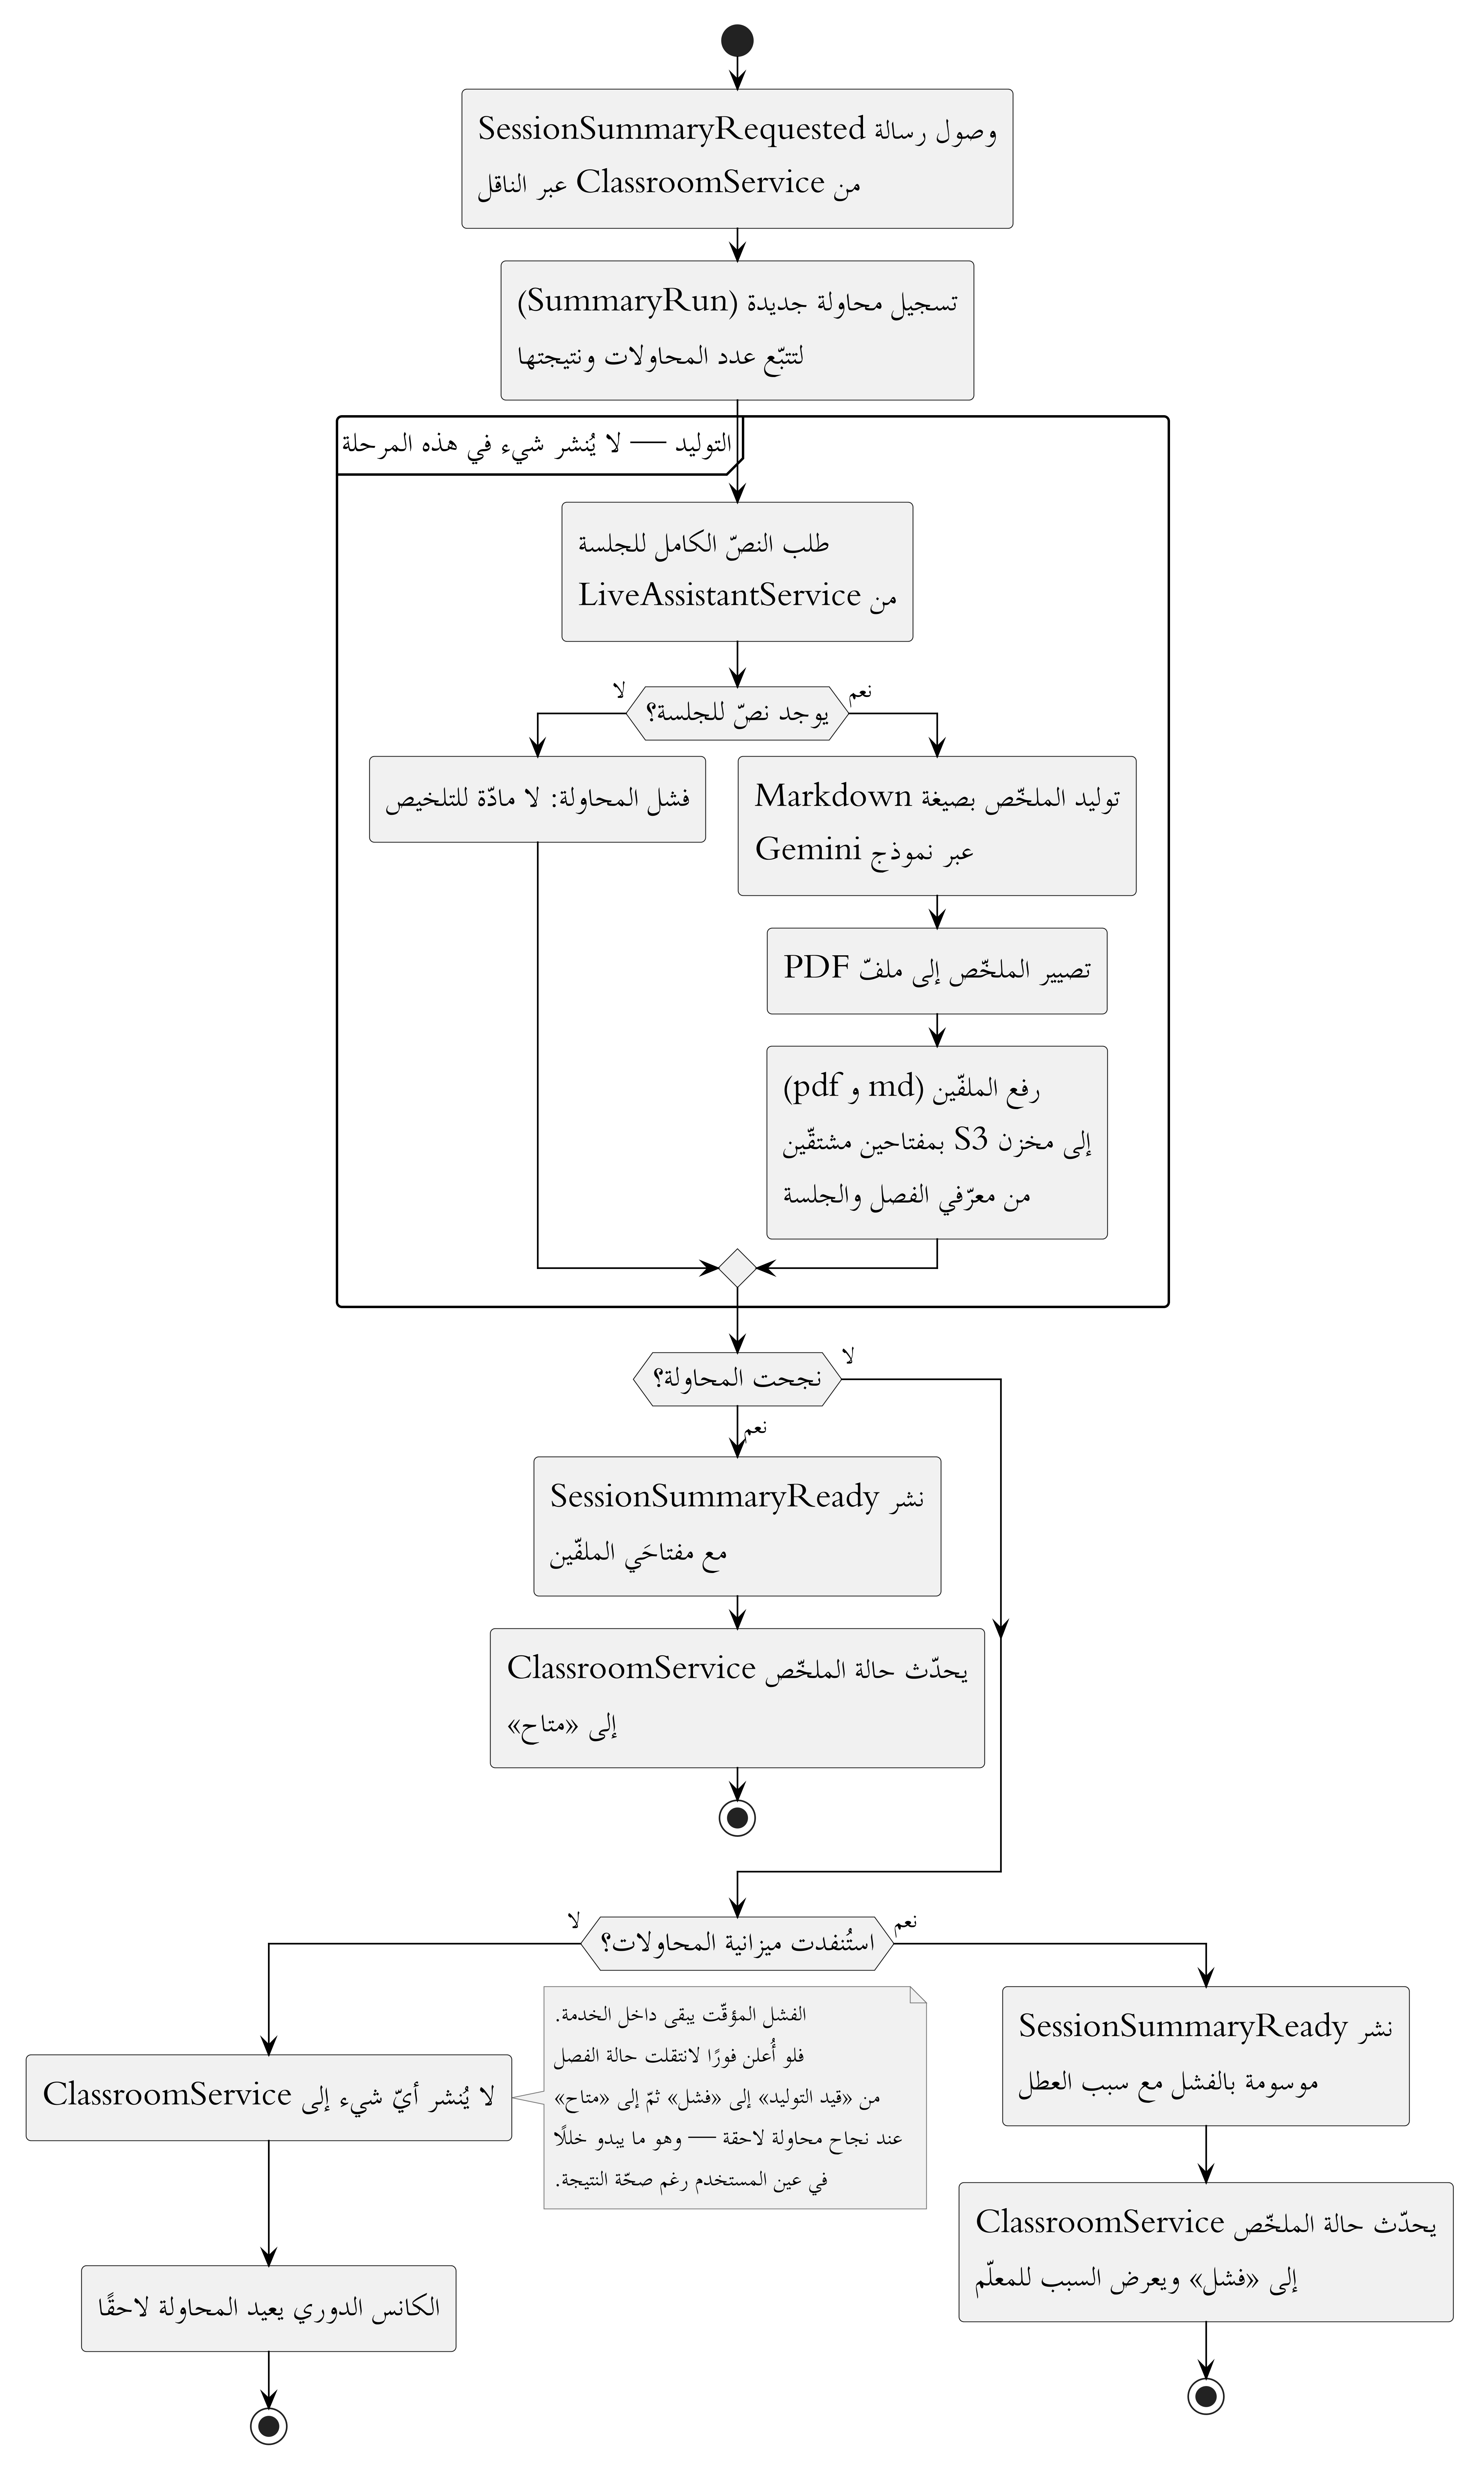
\includegraphics[width=\textwidth,height=0.8\textheight,keepaspectratio]{figures/arch-03b-session-summary.png}
  \caption{تدفّق توليد ملخّص الجلسة في خدمة الاسترجاع.}
  \label{fig:arch-03b}
\end{figure}

\noindent ويفصل هذا التدفّق بين التوليد والإعلان: فالمحاولة الفاشلة لا تنشر حدثاً ما دامت هناك محاولات باقية. ولولا هذا الفصل لانتقلت حالة الملخّص في واجهة الفصل من «قيد التوليد» إلى «فشل» ثمّ إلى «متاح» عند نجاح محاولة لاحقة، وهو تسلسل يظهر للمستخدم على أنّه خلل وإن كانت النتيجة النهائية صحيحة.

% ===========================================================================
% TODO(quiz-ssd): system sequence diagrams for the eight quiz use cases. Each
% figure block below is commented out and waiting for its PNG in figures/.
% Uncomment a block once its diagram exists — the file names are already chosen.
%   grep -n "TODO(quiz-ssd)" chapters/04-requirements-analysis.tex
% ===========================================================================
\subsection{مخطط تسلسل النظام لحالات استخدام الاختبارات}

\subsubsection{مخطط تسلسل النظام لحالة إنشاء مسودة اختبار وتوليدها}
% TODO(quiz-ssd)
\noindent [يُستكمل: مخطط تسلسل النظام لهذه الحالة.]
% \begin{figure}[htbp]
%   \centering
%   \includegraphics[width=\textwidth,height=0.8\textheight,keepaspectratio]{figures/ssd-quiz-01-compose.png}
%   \caption{مخطط تسلسل النظام لحالة «إنشاء مسودة اختبار وتوليدها».}
%   \label{fig:ssd-quiz-01}
% \end{figure}

\subsubsection{مخطط تسلسل النظام لحالة نشر الاختبار وإغلاقه أو إلغاؤه}
% TODO(quiz-ssd)
\noindent [يُستكمل: مخطط تسلسل النظام لهذه الحالة.]
% \begin{figure}[htbp]
%   \centering
%   \includegraphics[width=\textwidth,height=0.8\textheight,keepaspectratio]{figures/ssd-quiz-02-lifecycle.png}
%   \caption{مخطط تسلسل النظام لحالة «نشر الاختبار وإغلاقه أو إلغاؤه».}
%   \label{fig:ssd-quiz-02}
% \end{figure}

\subsubsection{مخطط تسلسل النظام لحالة تمديد مهلة الإجابة}
% TODO(quiz-ssd)
\noindent [يُستكمل: مخطط تسلسل النظام لهذه الحالة.]
% \begin{figure}[htbp]
%   \centering
%   \includegraphics[width=\textwidth,height=0.8\textheight,keepaspectratio]{figures/ssd-quiz-03-extend.png}
%   \caption{مخطط تسلسل النظام لحالة «تمديد مهلة الإجابة».}
%   \label{fig:ssd-quiz-03}
% \end{figure}

\subsubsection{مخطط تسلسل النظام لحالة استعراض نتائج الاختبار}
% TODO(quiz-ssd)
\noindent [يُستكمل: مخطط تسلسل النظام لهذه الحالة.]
% \begin{figure}[htbp]
%   \centering
%   \includegraphics[width=\textwidth,height=0.8\textheight,keepaspectratio]{figures/ssd-quiz-04-results.png}
%   \caption{مخطط تسلسل النظام لحالة «استعراض نتائج الاختبار».}
%   \label{fig:ssd-quiz-04}
% \end{figure}

\subsubsection{مخطط تسلسل النظام لحالة متابعة تحصيل الطلاب في الفصل الدراسي}
% TODO(quiz-ssd)
\noindent [يُستكمل: مخطط تسلسل النظام لهذه الحالة.]
% \begin{figure}[htbp]
%   \centering
%   \includegraphics[width=\textwidth,height=0.8\textheight,keepaspectratio]{figures/ssd-quiz-05-tracking.png}
%   \caption{مخطط تسلسل النظام لحالة «متابعة تحصيل الطلاب في الفصل الدراسي».}
%   \label{fig:ssd-quiz-05}
% \end{figure}

\subsubsection{مخطط تسلسل النظام لحالة الإجابة عن الاختبار وتسليمه}
% TODO(quiz-ssd)
\noindent [يُستكمل: مخطط تسلسل النظام لهذه الحالة.]
% \begin{figure}[htbp]
%   \centering
%   \includegraphics[width=\textwidth,height=0.8\textheight,keepaspectratio]{figures/ssd-quiz-06-answer.png}
%   \caption{مخطط تسلسل النظام لحالة «الإجابة عن الاختبار وتسليمه».}
%   \label{fig:ssd-quiz-06}
% \end{figure}

\subsubsection{مخطط تسلسل النظام لحالة الاطّلاع على نتيجة الاختبار}
% TODO(quiz-ssd)
\noindent [يُستكمل: مخطط تسلسل النظام لهذه الحالة.]
% \begin{figure}[htbp]
%   \centering
%   \includegraphics[width=\textwidth,height=0.8\textheight,keepaspectratio]{figures/ssd-quiz-07-my-result.png}
%   \caption{مخطط تسلسل النظام لحالة «الاطّلاع على نتيجة الاختبار».}
%   \label{fig:ssd-quiz-07}
% \end{figure}

\subsubsection{مخطط تسلسل النظام لحالة متابعة التحصيل الشخصي}
% TODO(quiz-ssd)
\noindent [يُستكمل: مخطط تسلسل النظام لهذه الحالة.]
% \begin{figure}[htbp]
%   \centering
%   \includegraphics[width=\textwidth,height=0.8\textheight,keepaspectratio]{figures/ssd-quiz-08-my-tracking.png}
%   \caption{مخطط تسلسل النظام لحالة «متابعة التحصيل الشخصي».}
%   \label{fig:ssd-quiz-08}
% \end{figure}
